\documentclass{article}
\usepackage{fixltx2e}
\usepackage{microtype}
%\usepackage{asymptote}
\usepackage{subcaption}

\usepackage{asypictureB}

\usepackage{tikz}
\usetikzlibrary{spy,positioning,shapes.geometric}
\usepackage{enumitem}
\usepackage{nicefrac}
\usepackage{booktabs}
\usepackage{amsmath,amssymb}
%\usepackage{wrapfig}
\usepackage{afterpage}
\usepackage{needspace}

% The maximum fraction of floats allowed at the top of a page:
\renewcommand{\topfraction}{0.9}

\newenvironment{danger}{\noindent\hangindent=3em\hangafter=-2%
  \clubpenalty=10000%
  \hbox to0pt{\hskip-\hangindent\smash{\tikz[baseline=1.3ex] \node[regular polygon, regular polygon sides=3, inner sep=0.05ex, very thick, line join=round, rounded corners=1pt, draw] (A) {\raisebox{0.2ex}{\textbf{\large!}}};}\hfill}\ignorespaces\textbf{\hspace*{-.2em}Warning:} \ignorespaces}%
  {\par}
\let\warning=\danger
\let\endwarning=\enddanger
  
\usepackage{makeidx}
\makeindex
%\usepackage{showidx}
\newcommand{\andfollowing}[1]{#1\textit{ff}}

\def \latex/{\LaTeX}

\newcommand{\raisedvdots}{\quad\smash{\raisebox{1ex}{\vdots}}}

\def\asylistingwidth{\dimexpr\linewidth-\myasywidth-7pt\relax}

\usepackage{environ}
%\usepackage{alltt}
%\RequirePackage{fancyvrb}
\RequirePackage{xcolor}
\usepackage{listings}
\lstset{language=C,
	breaklines=true,
	basicstyle=\ttfamily,
	breakatwhitespace=true,
	columns=flexible,
	keepspaces=true,
	numberblanklines=false,
	showstringspaces=false,
	commentstyle=\color{gray},
	backgroundcolor=\color{blue!10},
	frame=single,
	framerule=0pt,
	xleftmargin=3.01pt,
	xrightmargin=3.01pt,
	numberstyle=\footnotesize
	}
	
\newcommand{\mywidth}{}
	
\newif\ifinminipage
%
\newcommand{\begincodelisting}{%
\end{minipage}%
\inminipagetrue%
\hfill
\begin{minipage}[t]{\dimexpr\linewidth-\mywidth-7pt\relax}
\strut\par\vspace*{-\baselineskip}
\lstset{aboveskip=0pt}
}
%
\newcommand{\breakcodelisting}{%
\end{minipage}%
\inminipagefalse%
\begingroup%
\lstset{aboveskip=0pt}
}
%
\newenvironment*{asyexample}[1]%
{\par\bigskip%
\renewcommand{\mywidth}{#1}
\noindent
\begin{minipage}[t]{\mywidth}%
\mbox{}\\[-\baselineskip]}%
{\ifinminipage\end{minipage}\else\endgroup\fi\par\medskip}


\newcommand{\begingraphic}{%
\end{minipage}%
\hfill
\begin{minipage}[t]{\mywidth}%
\raggedleft%
\mbox{}\\[-\baselineskip]}
%
\newenvironment*{reverseasyexample}[1]%
{\par\bigskip%
\renewcommand{\mywidth}{#1}
\noindent
\begin{minipage}[t]{\dimexpr\linewidth-\mywidth-7pt\relax}
\strut\par\vspace*{-\baselineskip}
\lstset{aboveskip=0pt}%
}%
{\end{minipage}\par\medskip}

\let\Subsectionmark\subsectionmark
\def\subsectionmark#1{%
    \begingroup
        \catcode`\ =9%
        \catcode`;=9%
        \catcode`.=9%
        \catcode`(=9%
        \catcode`)=9%
        \catcode`[=9%
        \catcode`]=9%
        \catcode`,=9%
        \catcode`:=9%
        \catcode`{=9%
        \catcode`}=9%
        \catcode`\\=9%
        \everyeof{\noexpand}%
        \endlinechar=-1%
        \xdef\lastsectioningname{\scantokens{#1}}%
    \endgroup
    \Subsectionmark{#1}%
}
\let\Subsubsectionmark\subsubsectionmark
\def\subsubsectionmark#1{%
    \begingroup
        \catcode`\ =9%
        \catcode`;=9%
        \catcode`.=9%
        \catcode`(=9%
        \catcode`)=9%
        \catcode`[=9%
        \catcode`]=9%
        \catcode`,=9%
        \catcode`:=9%
        \catcode`{=9%
        \catcode`}=9%
        \catcode`\\=9%
        \everyeof{\noexpand}%
        \endlinechar=-1%
        \xdef\lastsectioningname{\scantokens{#1}}%
    \endgroup
    \Subsubsectionmark{#1}%
}

\asyset{name=\lastsectioningname}

\usepackage[hyphens]{url}
\usepackage[hidelinks]{hyperref}

%In case hyperref needs to be commented out:
\providecommand{\phantomsection}{}

\title{An Asymptote tutorial}
\author{Charles Staats III}
\date{\today}

\begin{document}
\begin{asyheader}
//settings.outformat="pdf";
real yellowPart = 0.4;
pen yellowPen = yellowPart*yellow + (1-yellowPart)*white + opacity(0.5);
pen yellowPenSolid = 0.5*(yellowPen + opacity(1.0)) + 0.5*white;
currentlight.background = yellowPenSolid;
void finish() { 
	currentlight.background = yellowPenSolid;
	if (settings.outformat != "png") shipout(bbox(yellowPen, Fill, xmargin=0.1cm)); 
}
pair topleft(picture pic) { return (pic.bounds.userMin().x, pic.bounds.userMax().y); }
pair topright(picture pic) {return pic.bounds.userMax(); }
pair bottomleft(picture pic) {return pic.bounds.userMin(); }
pair bottomright(picture pic) {return (pic.bounds.userMax().x, pic.bounds.userMin().y); }
\end{asyheader}
\maketitle
\tableofcontents
\section{First Steps}
\subsection{Introduction}
Janet is a calculus teacher. She is currently teaching her students how to find volumes of solids of revolution via the 
``disk method."  She would like to produce a diagram to illustrate the method---something like the diagram shown on 
page~\pageref{figure:target_diagram}.
%
\begin{figure}[t]
\centering
\begin{asypicture}{scale=0.25, name=ultimatetarget}
//Function to return a brace path
real innerangle = radians(60);
real outerangle = radians(70);
real midangle = radians(0);
path brace(pair a, pair b, real amplitude = .14*length(b-a)) {
  transform t = identity();
  real length = length(b-a);
  real sign = 1;
  if (amplitude < 0) {
    //    amplitude *= -1;
    sign = -1;
  }
  path brace = (0,0){expi(sign*outerangle)} :: {expi(sign*midangle)}(length/4, amplitude/2)
	      :: {expi(sign*innerangle)} (length/2, amplitude) {expi(-sign*innerangle)}
  :: {expi(-sign*midangle)}(3*length/4, amplitude/2) :: {expi(-sign*outerangle)} (length,0);
  real angle = degrees(atan2((b-a).y, (b-a).x));
  t = rotate(angle)*t;
  t = shift(a) * t;
  return t * brace;
}

//Define the command drawshifted, to be used later
void drawshifted(path g, pair trueshift, picture pic = currentpicture, Label label="", pen pen=currentpen, arrowbar arrow=None, arrowbar bar=None, margin margin=NoMargin, marker marker=nomarker)
{
  pic.add(new void(frame f, transform t) {
      picture opic;
      draw(opic, L=label, shift(trueshift)*t*g, p=pen, arrow=arrow, bar=bar,
	   margin=margin, marker=marker);
      add(f,opic.fit());
    });
  pic.addBox(min(g), max(g), trueshift+min(pen), trueshift+max(pen));
}

usepackage("amsmath");

real yellowPart = 0.2;
real unit = 2cm;
real truecm = cm / unit;
unitsize(unit);
pen backgroundpen = yellowPart*yellow + (1-yellowPart)*white;
frame finish() {
  currentlight.background = backgroundpen;
  frame toreturn = bbox(backgroundpen, Fill);
  currentpicture = new picture;
  unitsize(unit);
  return toreturn;
}

/*------------------------------*/

//Basic settings
settings.outformat="pdf";
defaultpen(fontsize(10pt));
import graph;

//Save some important numbers.
real xmin = -0.1;
real xmax = 2;
real ymin = -0.1;
real ymax = 2;

//Draw the graph and fill the area under it.
real f(real x) { return sqrt(x); }
path s = graph(f, 0, 2, operator..);
path fillregion = s -- (xmax,0) -- cycle;
pen fillpen = mediumgray;
fill(fillregion, fillpen);
draw(s, L=Label("$y=f(x)$", position=EndPoint));

//Fill the strip of width dx
real x = 1.4;
real dx = .05;
real t0 = times(s,x)[0];
real t1 = times(s,x+dx)[0];
path striptop = subpath(s,t0,t1);
filldraw((x,0) -- striptop -- (x+dx,0) --  cycle, black);

//Draw the bars labeling the width dx
real barheight = f(x+dx);
pair barshifty = (0, 0.2cm);
Label dxlabel = Label("$dx$", position=MidPoint, align=2N);
drawshifted((x,barheight) -- (x+dx, barheight), trueshift=barshifty, label=dxlabel, bar=Bars);

//Draw the arrows pointing inward toward the dx label
real myarrowlength = 0.3cm;
margin arrowmargin = DotMargin;
path leftarrow = shift(barshifty) * ((-myarrowlength, 0) -- (0,0));
path rightarrow = shift(barshifty) * ((myarrowlength, 0) -- (0,0));
draw((x, barheight), leftarrow, arrow=Arrow(), margin=arrowmargin);
draw((x+dx, barheight), rightarrow, arrow=Arrow(), margin=arrowmargin);

//Draw the bar labeling the height f(x)
real barx = x + dx;
pair barshiftx = (0.42cm, 0);
Label fxlabel = Label("$f(x)$", align=(0,0), position=MidPoint, filltype=Fill(fillpen));
drawshifted((barx,0) -- (barx, f(x)), trueshift=barshiftx, label=fxlabel, arrow=Arrows(), bar=Bars); 

//Draw the axes on top of everything that has gone before
arrowbar axisarrow = Arrow(TeXHead);
Label xlabel = Label("$x$", position=EndPoint);
draw((xmin,0) -- (xmax,0), arrow=axisarrow, L=xlabel);
Label ylabel = Label("$y$", position=EndPoint);
draw((0,ymin) -- (0,ymax), arrow = axisarrow, L=ylabel);

//Draw the tick mark on the x-axis
path tick = (0,0) -- (0,-0.15cm);
Label ticklabel = Label("$x$", position=EndPoint);
draw((x,0), tick, L=ticklabel);

frame pic2dFrame = finish();

/* ----------------------------------------------------- */

settings.prc = false;
settings.render=16;
import three;

currentprojection = orthographic(5,0,10, up=Y);
//currentprojection=oblique;
//currentprojection=perspective(6,0,10,up=Y);

pen color = white;
material surfacepen = material(diffusepen=color+opacity(1.0), emissivepen=0.2*color);
material planepen = material(diffusepen=opacity(0.6), emissivepen=0.8*color);
pen diskpen = black+opacity(1.0);

path3 p3 = path3(s);
draw(p3);

surface FilledRegion = surface(fillregion);
draw(FilledRegion, surfacepen = gray(0.6) + opacity(0.8));

surface solidsurface = surface(p3, c=O, axis=X);
draw(solidsurface, surfacepen=surfacepen);

/*
int n = length(p3);
for (real i = 0; i <= n; i += n/10) {
  if (i >= n) i -= .01;
  draw(solidsurface.vequals(i), gray(0.3));
}
*/
draw(solidsurface.vequals(length(p3) - .001), gray(0.3));

real extra = 0.4 truecm;
path planeboundary = (xmin,ymin) -- (xmax+extra,ymin) -- (xmax+extra,ymax+extra) -- (xmin,ymax+extra) -- cycle;
path planeoutside = planeboundary -- fillregion -- cycle;
draw(surface(planeoutside), surfacepen=planepen);

transform pushoutside = shift(0,.001);
striptop = pushoutside*striptop;
path3 dVtop = path3(striptop);
path3 openStrip = (x,0,0) -- dVtop -- (x+dx,0,0);
surface disk = surface(openStrip, c=O, axis=X);
draw(disk, diskpen);

triple cameraDirection(triple pt, projection P = currentprojection) {
  if (P.infinity) {
    return unit(P.camera);
  } else {
    return unit(P.camera - pt);
  }
}

triple towardCamera(triple pt, real dist = 1 truecm, projection P = currentprojection) {
  return pt + dist*cameraDirection(pt, P);
}

draw(xmin*X -- xmax*X, arrow=Arrow3(TeXHead2(normal=Z)));
draw(ymin*Y -- ymax*Y, arrow=Arrow3(TeXHead2(normal=Z)));
label("$x$", position=towardCamera(xmax*X), align = E);
label("$y$", position=towardCamera(ymax*Y), align=N);

frame pic3dFrame = finish();

/* ----------------------------------------------------- */

currentprojection=orthographic((3,0,10), up=Y);

diskpen = mediumgray;
draw(disk, diskpen);

transform3 T = rotate(10, X);
path3 brace = T*path3(brace((x+dx,barheight), (x+dx,0)));
draw(brace--cycle);
label("$r=f(x)$", position=midpoint(brace), align=E);

//Draw the bars labeling the width dx
path3 dxlabelpath = T * ((x, barheight, 0) -- (x+dx, barheight, 0));
draw(dxlabelpath, L=dxlabel, Bars3);

arrow(relpoint(dxlabelpath,0), dir=W, length=myarrowlength, margin=DotMargin3, arrow=Arrow3(emissive(black)));
arrow(relpoint(dxlabelpath,1), dir=E, length=myarrowlength, margin=DotMargin3, arrow=Arrow3(emissive(black)));

draw(xmin*X -- xmax*X, arrow=Arrow3(TeXHead2(normal=Z)));
draw(ymin*Y -- ymax*Y, arrow=Arrow3(TeXHead2(normal=Z)));
label("$x$", position=towardCamera(xmax*X), align = E);
label("$y$", position=towardCamera(ymax*Y), align=N);

frame oneSlice = finish();
/* ----------------------------------------------------- */

label(minipage("\raggedright Dimensions of infinitesimally thin sheet: 
\begin{description}
\item[Area:] $\pi r^2 = \pi [f(x)]^2$
\item[Thickness:] $dx$
\item[Volume:] $dV = \text{Area}\cdot\text{thickness} = \pi [f(x)]^2\;dx$
\end{description}"
,6cm));

frame labelFrame = finish();

/* ----------------------------------------------------- */

unit = 1;
unitsize(unit);
add(pic3dFrame);
add(labelFrame, position=(max(pic3dFrame).x, min(pic3dFrame).y - 1cm), align=SW);
pic3dFrame = finish();

/* ----------------------------------------------------- */

//unitsize(1);    // Set the usual (postscript) coordinates.
add(pic2dFrame);
add(pic3dFrame, position=max(pic2dFrame), align=SE);
add(oneSlice, position=min(pic2dFrame)+(0,-1cm), align=SE);

// Scale up by 4 in order to increase resolution.
shipout(scale(4)*finish());
\end{asypicture}
\label{figure:target_diagram}
\end{figure}
\par As an experienced user of TikZ\index{TikZ}, Janet does not think she would have trouble producing the diagram in the top left of 
the figure. She also believes she could get the diagram in the bottom left with some fiddling. However, she simply does 
not believe the three-dimensional capabilities of TikZ are up to drawing a diagram like that in the top right---at least, 
not without far more time and fiddling than Janet is willing to put in for a single diagram.

Janet's husband Vincent is a programmer. He has some familiarity with the programming language Asymptote, which 
is especially designed to produce vector graphics and has some fairly substantial three-dimensional capabilities. Working with 
her husband, Janet decides to try to draw the figure using Asymptote.

\subsection{Hello World}
Janet already has an up-to-date installation of TeXLive.  On the off-chance that this includes an Asymptote installation, 
she attempts a simple Hello World program. She uses her favorite
 text editor\footnote{She is inclined to use TeXShop\index{TeXShop}, 
 since she already has it, but Aquamacs\index{Aquamacs} would 
 really be more suitable.  Vincent, who is a die-hard fan of the command line, recommends using 
 the command-line editor \texttt{nano}\index{nano@\texttt{nano} text editor}.  
 On a Windows machine, the simplest thing to use would 
 be Notepad\index{Notepad}.} 
to produce a document consisting of the single line
\index{label@\texttt{label()}}
\begin{lstlisting}
label("Hello world!");
\end{lstlisting}
and saves it as \verb|hello_world.asy|\index{helloworld@\texttt{hello\_world.asy}}. 
She then goes to the command line and types \verb|asy hello_world|\index{asy@\texttt{asy}}. The result is 
an eps file named \verb|hello_world.eps|.  Opening it, she sees a single page with the following printed on it:\footnote{Not including 
the yellow background, of course.}
\begin{center}
\begin{asypicture}{name=hello_world}
settings.outformat="pdf";
defaultpen(fontsize(12));
label("Hello world!");
finish();
\end{asypicture}
\end{center}
Thus, to the surprise of both Janet and her husband, it appears that Asymptote is already installed on her computer.\footnote{This 
was more or less my experience, working on Mac OS X. If you are not fortunate enough to have had this miracle happen to you, 
see Appendix \ref{appendix:installing} and the installation instructions in the Asymptote manual.}

Since Janet uses \verb|pdflatex|\index{pdflatex}, she finds it annoying to import eps\index{eps} files, and would prefer that the ``graphic" be output in 
another format.  Adding one line to her Asymptote file causes it to output a pdf file instead:
\index{settingsoutformat@\texttt{settings.outformat}}\label{settingsoutformat}
\begin{lstlisting}
settings.outformat = "pdf";
label("Hello world!");
\end{lstlisting}
Vincent notes that every line should end with a semicolon\index{semicolon}.  
Since TikZ behaves the same way, Janet does not find this too 
difficult to remember.

Now that Janet has a pdf file containing her ``graphic," she decides to import it into a latex file. Having done so, she is 
pleased to notice that Hello World is printed in the same font as the rest of her document (Computer Modern). However, she 
considers it unfortunate that the font size in the ``graphic" is larger than in the rest of her document.  Vincent asks her what size 
she would like the font in her Asymptote graphics. Being told that the desired font size is 10 points, he proposes the following:
\index{font size}\index{defaultpen@\texttt{defaultpen()}}\index{fontsize@\texttt{fontsize()}}\index{pen!fontsize@\texttt{fontsize()}}
\begin{lstlisting}
settings.outformat = "pdf";
defaultpen(fontsize(10pt));
label("Hello world!");
\end{lstlisting}
The result is 
\begin{center}
\begin{asypicture}{name=hello_world}
settings.outformat = "pdf";
defaultpen(fontsize(10pt));
label("Hello world!");
finish();
\end{asypicture}
\end{center}
which looks nicer with the rest of the document.

\subsection{Interpreting the documentation}\label{section:interpretdoc}
The \verb|label()|\index{label@\texttt{label()}|(} command used in the Asymptote code above is described in Section 4.4 of the Asymptote manual\index{manual}\index{asymanual@Asymptote manual},
with the following declaration:
\begin{lstlisting}
void label(picture pic=currentpicture, Label L, pair position,
           align align=NoAlign, pen p=currentpen, 
           filltype filltype=NoFill)
\end{lstlisting}
Janet finds this a bit overwhelming. Vincent suggests that she ignore everything with an \verb'=' sign in it, 
since those are all optional arguments,\index{optional arguments} and think of such a declaration simply as 
\begin{lstlisting}
label(Label L, pair position);
\end{lstlisting}
Essentially, if Janet wants to use this command to add a label to her picture, she should tell what Label to add 
and where to add it. For instance, the line 
\begin{lstlisting}
label("Hello world", (0,0));
\end{lstlisting}
would add the text ``Hello world" to the picture at position $(0,0)$.  Given this description, Janet wonders why the program
she already wrote worked; shouldn't she have been required to specify a position?  Vincent confirms that 
according to the documentation, the line \verb'label("Hello world");' without any position should not have worked.  He admits 
that the documentation is sometimes not completely accurate, which Janet does not find encouraging.

It seems rather peculiar to Janet that the equals sign should be what indicates that an argument can be ignored. 
Vincent explains that the equals sign provides a default\index{default~argument} value; when there is a default value, the program knows what to 
do if the user does not specify a value.

Here are the optional arguments for the \verb'label' command:
\begin{center}
\begin{tabular}{@{} l l l @{}}						\toprule
type			& name			& default value		\\ \midrule
\verb'picture'	& \verb'pic'		& \verb'currentpicture'	\\
\verb'align'	& \verb'align'		& \verb'NoAlign'	\\
\verb'pen'		& \verb'p'			& \verb'currentpen'	\\
\verb'filltype'	& \verb'filltype'		& \verb'NoFill'		\\ \bottomrule
\end{tabular}
\end{center}
These optional arguments behave something like key-value\index{key-value} assignments.
For instance, if Janet had wanted to change the text size of just the single line, rather than the entire picture, she could 
have set the key \verb;p;\index{pen@\texttt{pen}} to value \verb;fontsize(10pt);\index{fontsize@\texttt{fontsize()}} as follows:
\begin{lstlisting}
settings.outformat = "pdf";
label("Hello world", p = fontsize(10pt));
\end{lstlisting}
Note that \verb;fontsize(10pt); is an object of type \verb;pen;, just as \verb;"Hello world"; (including the quotation marks) 
is an object of type \verb;Label;.\footnote{Technically, \texttt{"Hello world"} is of type \texttt{string}\index{string@\texttt{string}}, but strings can
be treated as Labels in Asymptote.}
The output is the same as before, since the picture has only one piece of text:\index{label@\texttt{label()}|)}
\begin{center}
\begin{asypicture}{name=hello_world}
settings.outformat = "pdf";
label("Hello world", p = fontsize(10pt));
finish();
\end{asypicture}
\end{center}
Janet asks how to define a single key that can set several others, as in TikZ styles\index{TikZ!styles}.  
Vincent says that this is not 
possible in Asymptote, although he can see how it might be useful.

\section{Drawing a two-dimensional image}
\subsection{Lines and sizing}
Having determined that Asymptote is already installed on her computer, Janet decides to use it to draw a 
picture of the two-dimensional region that will be revolved.  She could do this using TikZ, but Vincent recommends 
that she get some basic practice drawing with Asymptote before tackling a three-dimensional picture.  Here is, 
roughly, what Janet would like:
\begin{center}
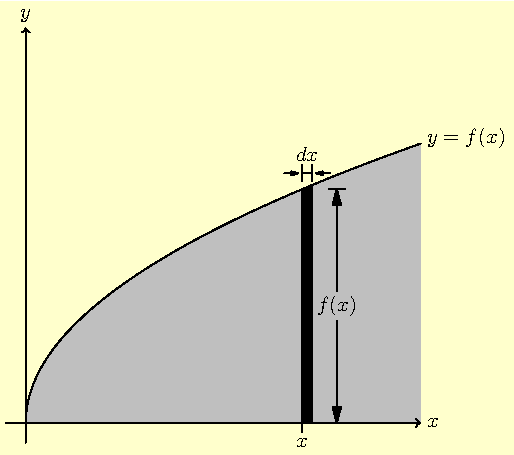
\includegraphics{disk-method-2d.pdf}
\end{center}
First of all, she tries drawing the $x$-axis as a line\index{line} 
from $(-0.1, 0)$ to $(2,0)$, and the $y$-axis as a line 
from $(0,-.1)$ to $(0,2)$;

\bigskip
\noindent\begin{minipage}{\textwidth}
\begin{minipage}[c]{0.4\textwidth}
\vspace{0pt}
\begin{lstlisting}
settings.outformat="pdf";
draw((-.1,0) -- (2,0));
draw((0,-.1) -- (0,2));
\end{lstlisting}
\index{draw@\texttt{draw()}}\index{draw@\texttt{draw()}!line}
\index{--operator@\texttt{--} operator!drawing}
\end{minipage}
\hfill
\begin{minipage}[c]{0.5\textwidth}
\vspace{0pt}
\begin{asypicture}{name=line_too_small}
settings.outformat = "pdf";
draw((-.1,0) -- (2,0));
draw((0,-.1) -- (0,2));
finish();
\end{asypicture}
\end{minipage}
\end{minipage}

\bigskip
The result is a mark that is barely visible because it is so short. Vincent lets Janet know this is because, by 
default, Asymptote interprets one unit\index{unit} to mean one point\index{point, unit of measurement}---roughly $0.035$ centimeters. 
Janet thinks that the TikZ default of 1 centimeter is 
much more reasonable.  This can be arranged by 
adding the line \texttt{unitsize(1cm);}\index{unitsize@\texttt{unitsize()}} to the code:

\begin{asyexample}{2.4cm}
\begin{asypicture}{name=simple_line}
settings.outformat="pdf";
unitsize(1cm);
draw((-.1,0) -- (2,0));
draw((0,-.1) -- (0,2));
finish();
\end{asypicture}
\begincodelisting
\begin{lstlisting}
settings.outformat="pdf";
unitsize(1cm);
draw((-.1,0) -- (2,0));
draw((0,-.1) -- (0,2));
\end{lstlisting}
\end{asyexample}
\noindent The final product should be larger still, but is kept this size for now to save space.

There's one more kind of sizing option for Asymptote: the \lstinline;size; command.\index{size@\texttt{size()}|(} 
In its simplest 
usage, this command takes a single length for an argument---in the code below, \lstinline;3cm;---and makes the 
final picture as large as possible, keeping the same height-to-width ratio, 
such that neither the width nor the height exceeds the specified dimension 
(3 centimeters).

\begin{asyexample}{3.2cm}
\begin{asypicture}{name=size_command}
settings.outformat="pdf";
size(3cm);
draw((-.1,0) -- (2,0));
draw((0,-.1) -- (0,2));
finish();
\end{asypicture}
\begincodelisting
\begin{lstlisting}
settings.outformat="pdf";
size(3cm);
draw((-.1,0) -- (2,0));
draw((0,-.1) -- (0,2));
\end{lstlisting}
\end{asyexample}
\noindent
The \lstinline;size; command has several important variations:
\begin{itemize}
\item \lstinline!size(real, real)! takes two dimensions---a maximum width and a maximum height, 
in that order.  Thus, for instance, 
code that begins with the command \lstinline!size(2cm, 3cm);! will ordinarily produce a picture that is 
either 2 centimeters wide (and $\leq 3$ centimeters tall) or a picture that is 3 centimeters tall (and 
$\leq 2$ centimeters wide).  In either case, the height-to-width\index{height-to-width ratio} ratio is preserved.
\item If either argument in \lstinline!size(real, real)! is zero, it is ignored.  Thus, for instance, 
a picture that includes the command \lstinline!size(4cm, 0);! will ordinarily be scaled so that the 
width is exactly 4 centimeters.  The height will be the ``natural" height for this scaling factor.
\item The command \lstinline!size(real, real, keepAspect=false);!\index{keepAspect=@\texttt{keepAspect=}}\index{size@\texttt{size()}!keepAspect=@\texttt{keepAspect=}} will scale the width and height 
independently so that the resulting picture has exactly the specified width and height, but the height-to-width 
ratio is allowed to change.  Thus, for instance, if a circle is drawn on a picture that has this type of 
size command, the circle is likely to end up looking like an ellipse.\index{size@\texttt{size()}|)}
\end{itemize}
One of Janet's frustrations with TikZ has been that it is difficult to produce a picture that has exactly 
the desired width (or height).  She is gratified to learn that this will be much easier with Asymptote.

\subsection{Arrowheads}
\index{arrows|(}
With the axis lines drawn, Janet thinks that they should have arrows indicating the directions. 
Vincent agrees that the axes should have arrows. Janet's students do not care about arrows.

Arrows can be added on the end of the line by using the optional parameter 
\texttt{arrow}\index{arrow=@\texttt{arrow=}} in the 
draw command:

\bigskip
\noindent\begin{minipage}{\textwidth}
\begin{minipage}[b]{0.6\textwidth}
\vspace{0pt}
\begin{lstlisting}
settings.outformat="pdf";
unitsize(1cm);
draw((-.1,0) -- (2,0), arrow=Arrow);
draw((0,-.1) -- (0,2), arrow = Arrow);
\end{lstlisting}
\end{minipage}
\hfill
\begin{asypicture}{name=plain_arrow}
settings.outformat="pdf";
unitsize(1cm);
draw((-.1,0) -- (2,0), arrow=Arrow);
draw((0,-.1) -- (0,2), arrow = Arrow);
finish();
\end{asypicture}
\end{minipage}

\bigskip
\noindent Vincent thinks this looks fairly nice.  Janet wants to imitate the \TeX-style arrowheads 
$\rightarrow$, as she is used to being done in TikZ.  Looking in the Asymptote manual, 
she and Vincent find the following styles for arrowheads:
\begin{center}
\begin{tabular}{@{}l l@{}}		\toprule
Asymptote code & appearance \\ \midrule
\verb'draw((0,0)--(1,0),arrow=Arrow());'\index{Arrow@\texttt{Arrow()}}\index{arrow=@\texttt{arrow=}!Arrow@\texttt{Arrow()}} &
\begin{asypicture}{name=arrow_table}
settings.outformat = "pdf"; unitsize(1cm);  draw((0,0)--(1,0), arrow=Arrow()); finish();
\end{asypicture}
\\
\verb'draw((0,0)--(1,0),arrow=ArcArrow());'\index{ArcArrow@\texttt{ArcArrow()}}\index{arrow=@\texttt{arrow=}!ArcArrow@\texttt{ArcArrow()}} &
\begin{asypicture}{name=arrow_table}
settings.outformat = "pdf"; unitsize(1cm);  draw((0,0)--(1,0), arrow=ArcArrow()); finish();
\end{asypicture}
\\ 
\verb'draw((0,0)--(1,0),arrow=Arrow(SimpleHead));'\index{SimpleHead@\texttt{SimpleHead}}\index{arrow=@\texttt{arrow=}!ArrowSimpleHead@\texttt{Arrow(SimpleHead)}} &
\begin{asypicture}{name=arrow_table}
settings.outformat = "pdf"; unitsize(1cm);  draw((0,0)--(1,0), arrow=Arrow(SimpleHead)); finish();
\end{asypicture}
\\
\verb'draw((0,0)--(1,0),arrow=ArcArrow(SimpleHead));'\index{arrow=@\texttt{arrow=}!ArcArrowSimpleHead@\texttt{ArcArrow(SimpleHead)}} &
\begin{asypicture}{name=arrow_table}
settings.outformat = "pdf"; unitsize(1cm);  draw((0,0)--(1,0), arrow=ArcArrow(SimpleHead)); finish();
\end{asypicture}
\\
\verb'draw((0,0)--(1,0),arrow=Arrow(HookHead));'\index{HookHead@\texttt{HookHead}}\index{arrow=@\texttt{arrow=}!ArrowHookHead@\texttt{Arrow(HookHead)}} &
\begin{asypicture}{name=arrow_table}
settings.outformat = "pdf"; unitsize(1cm);  draw((0,0)--(1,0), arrow=Arrow(HookHead)); finish();
\end{asypicture}
\\
\verb'draw((0,0)--(1,0),arrow=ArcArrow(HookHead));'\index{arrow=@\texttt{arrow=}!ArcArrowHookHead@\texttt{ArcArrow(HookHead)}} &
\begin{asypicture}{name=arrow_table}
settings.outformat = "pdf"; unitsize(1cm);  draw((0,0)--(1,0), arrow=ArcArrow(HookHead)); finish();
\end{asypicture}
\\
\verb'draw((0,0)--(1,0),arrow=Arrow(TeXHead));'\index{TeXHead@\texttt{TeXHead}}\index{arrow=@\texttt{arrow=}!ArrowTeXHead@\texttt{Arrow(TeXHead)}} &
\begin{asypicture}{name=arrow_table}
settings.outformat = "pdf"; unitsize(1cm);  draw((0,0)--(1,0), arrow=Arrow(TeXHead)); finish();
\end{asypicture}
\\
\bottomrule
\end{tabular}
\end{center}
The last, the \verb'TeXHead' style, is more what Janet has in mind:

\begin{asyexample}{2.3cm}
\begin{asypicture}{name=TeXHead}
settings.outformat="pdf";
unitsize(1cm);
draw((-.1,0) -- (2,0), arrow=Arrow(TeXHead));
draw((0,-.1) -- (0,2), arrow = Arrow(TeXHead));
finish();
\end{asypicture}
\begincodelisting
\begin{lstlisting}
settings.outformat="pdf";
unitsize(1cm);
draw((-.1,0) -- (2,0), arrow=Arrow(TeXHead));
draw((0,-.1) -- (0,2), arrow = Arrow(TeXHead));
\end{lstlisting}
\end{asyexample}
\index{arrows|)}

\subsection{Curved paths}
\index{curved paths|(}\index{draw@\texttt{draw()}!path|(}
Next, Janet would like to draw the parabola function, which is supposed to look something 
like the graph of $y = \sqrt{x}$.   Here's a first attempt, with a path through the three points 
$(0,0)$, $(1,1)$, and $(2,\sqrt{2})$:

\bigskip
\noindent\begin{minipage}{\textwidth}
\begin{minipage}[b]{0.6\textwidth}
\vspace{0pt}
\begin{lstlisting}
settings.outformat="pdf";
unitsize(1cm);
draw((-.1,0) -- (2,0), arrow=Arrow(TeXHead));
draw((0,-.1) -- (0,2), arrow = Arrow(TeXHead));
draw((0,0) -- (1,1) -- (2,sqrt(2)));
\end{lstlisting}
\index{square root}\index{sqrt@\texttt{sqrt()}}
\end{minipage}
\hfill
\begin{asypicture}{name=parabola}
settings.outformat="pdf";
unitsize(1cm);
draw((-.1,0) -- (2,0), arrow=Arrow(TeXHead));
draw((0,-.1) -- (0,2), arrow = Arrow(TeXHead));
draw((0,0) -- (1,1) -- (2,sqrt(2)));
finish();
\end{asypicture}
\end{minipage}

\bigskip\noindent This does not look very nice at all. Substituting \verb'..' for the connector 
\verb'--' can at least make the path look smooth:

\bigskip
\noindent\begin{minipage}{\textwidth}
\begin{minipage}[b]{0.6\textwidth}
\vspace{0pt}
\begin{lstlisting}
settings.outformat="pdf";
unitsize(1cm);
draw((-.1,0) -- (2,0), arrow=Arrow(TeXHead));
draw((0,-.1) -- (0,2), arrow = Arrow(TeXHead));
draw((0,0) .. (1,1) .. (2,sqrt(2)));
\end{lstlisting}
\end{minipage}
\index{..operator@\texttt{..} operator|(}
\hfill
\begin{asypicture}{name=parabola}
settings.outformat="pdf";
unitsize(1cm);
draw((-.1,0) -- (2,0), arrow=Arrow(TeXHead));
draw((0,-.1) -- (0,2), arrow = Arrow(TeXHead));
draw((0,0) .. (1,1) .. (2,sqrt(2)));
finish();
\end{asypicture}
\end{minipage}

\bigskip\noindent
While this is a significant improvement, Janet would also like to make the tangent at the 
origin vertical. This can also be specified:

\bigskip
\noindent\begin{minipage}{\textwidth}
\begin{minipage}[b]{0.6\textwidth}
\begin{lstlisting}
settings.outformat="pdf";
unitsize(1cm);
draw((-.1,0) -- (2,0), arrow=Arrow(TeXHead));
draw((0,-.1) -- (0,2), arrow = Arrow(TeXHead));
draw((0,0){up} .. (1,1) .. (2,sqrt(2)));
\end{lstlisting}
\end{minipage}
\index{tangent direction|(}
\hfill
\begin{asypicture}{name=parabola_vertical_tangent}
settings.outformat="pdf";
unitsize(1cm);
draw((-.1,0) -- (2,0), arrow=Arrow(TeXHead));
draw((0,-.1) -- (0,2), arrow = Arrow(TeXHead));
draw((0,0){up} .. (1,1) .. (2,sqrt(2)));
finish();
\end{asypicture}
\end{minipage}

\bigskip\noindent
This looks more or less like what Janet had in mind.

Note that \verb'up'\index{up@\texttt{up}} is really just short for \verb`(0,1)`. If Janet wanted a direction 
other than \verb'up' (or \texttt{down}\index{down@\texttt{down}}, \texttt{right}\index{right@\texttt{right}}, or \texttt{left}\index{left@\texttt{left}}, which are similar), 
she could specify the tangent direction explicitly as an ordered pair.  For instance, here is a rough 
approximation of a sine curve:

\bigskip
\noindent\begin{minipage}{\textwidth}
\begin{minipage}[c]{0.6\textwidth}
\begin{lstlisting}
settings.outformat = "pdf";
unitsize(0.5cm);
draw((0,0){(1,1)} .. {right}(pi/2,1) 
      .. {(1,-1)}(pi,0) .. {right}(3*pi/2,-1) 
      .. {(1,1)}(2*pi, 0));
\end{lstlisting}
\end{minipage}
\hfill
\begin{asypicture}{name=sine_curve}
settings.outformat = "pdf";
unitsize(0.5cm);
draw((0,0){(1,1)} .. {right}(pi/2,1) 
      .. {(1,-1)}(pi,0) .. {right}(3*pi/2,-1) 
      .. {(1,1)}(2*pi, 0));
finish();
\end{asypicture}
\end{minipage}

\medskip\noindent
Without the tangent directions specified, Asymptote does a very nice job of connecting the 
dots to form a smooth curve, but it doesn't really look like a sine curve.  The ends in particular
are much too steep:

\medskip
\noindent\begin{minipage}{\textwidth}
\begin{minipage}[c]{0.6\textwidth}
\begin{lstlisting}
settings.outformat = "pdf";
unitsize(0.5cm);
draw((0,0) .. (pi/2,1) .. (pi,0) 
      .. (3*pi/2,-1) .. (2*pi, 0));
\end{lstlisting}
\end{minipage}
\hfill
\begin{asypicture}{name=bad_sine_curve}
settings.outformat = "pdf";
unitsize(0.5cm);
draw((0,0) .. (pi/2,1) .. (pi,0) 
      .. (3*pi/2,-1) .. (2*pi, 0));
finish();
\end{asypicture}
\end{minipage}

\medskip
Except at the first and last points, the tangent direction at a point can be specified 
either before or after the point---or, if a corner is desired, at both:

\medskip
\noindent\begin{minipage}{\textwidth}
\begin{minipage}[c]{0.6\textwidth}
\begin{lstlisting}
settings.outformat = "pdf";
unitsize(0.5cm);
draw((0,2) .. {(1,-3)}(2,0){(1,1/3)} .. (4,2));
\end{lstlisting}
\end{minipage}
\hfill
\begin{asypicture}{name=tangent_everywhere}
settings.outformat = "pdf";
unitsize(0.5cm);
draw((0,2) .. {(1,-3)}(2,0){(1,1/3)} .. (4,2));
finish();
\end{asypicture}
\end{minipage}
\index{curved paths|)}\index{tangent direction|)}\index{..operator@\texttt{..} operator|)}\index{draw@\texttt{draw()}!path|)}

\subsection{Markers on paths}
If Janet wants to see what the points on a path were actually specified, she can use the 
\verb;marker;\index{marker=@\texttt{marker=}} option to the \verb;draw;\index{draw@\texttt{draw()}!marker=@\texttt{marker=}} command:

\medskip\noindent
\begin{minipage}{0.6\textwidth}
\vspace{0pt}
\begin{lstlisting}
settings.outformat="pdf";
unitsize(0.5cm);
draw((0,0) .. (pi/2,1) .. (pi,0) 
      .. (3*pi/2,-1) .. (2*pi, 0), 
      marker=MarkFill[0]);
\end{lstlisting}
\end{minipage}
\hfill
\begin{minipage}{0.38\textwidth}
\vspace{0pt}
\begin{asypicture}{name = markers}
settings.outformat="pdf";
unitsize(0.5cm);
draw((0,0) .. (pi/2,1) .. (pi,0) 
      .. (3*pi/2,-1) .. (2*pi, 0), 
      marker=MarkFill[0]);
finish();
\end{asypicture}
\end{minipage}

\medskip\noindent
Designing your own markers is not that difficult, but requires more knowledge than is currently
available.  Here are the built-in markers: {
\newcommand{\asywidth}{2.36cm}
\renewcommand{\arraystretch}{1.8}
\begin{center}
\begin{tabular}{@{}l l l@{}}
\toprule
built-in option 		& description 	& appearance \\	\midrule
\verb;Mark[0]; 		& open circle	&
\begin{minipage}[c]{\asywidth}
\vspace{0pt}
\begin{asypicture}{name=markertable}
settings.outformat="pdf";
unitsize(.7cm);
draw((0,0) -- (1,.5){right} .. (2,.5) .. (3,0) ^^ (1.5,0), marker=Mark[0]);
finish();
\end{asypicture}
\end{minipage}
\\
\verb;MarkFill[0]; 		& filled circle	&
\begin{minipage}[c]{\asywidth}
\vspace{0pt}
\begin{asypicture}{name=markertable}
settings.outformat = "pdf";
unitsize(.7cm);
draw((0,0) -- (1,.5){right} .. (2,.5) .. (3,0) ^^ (1.5,0), marker=MarkFill[0]);
finish();
\end{asypicture}
\end{minipage}
\\
\verb;Mark[1];		& open triangle	&
\begin{minipage}[c]{\asywidth}
\vspace{0pt}
\begin{asypicture}{name=marker}
settings.outformat = "pdf";
unitsize(.7cm);
draw((0,0) -- (1,.5){right} .. (2,.5) .. (3,0) ^^ (1.5,0), marker=Mark[1]);
finish();
\end{asypicture}
\end{minipage}
\\
\verb;MarkFill[1];		& filled triangle	&
\begin{minipage}[c]{\asywidth}
\vspace{0pt}
\begin{asypicture}{name=marker}
settings.outformat = "pdf";
unitsize(.7cm);
draw((0,0) -- (1,.5){right} .. (2,.5) .. (3,0) ^^ (1.5,0), marker=MarkFill[1]);
finish();
\end{asypicture}
\end{minipage}
\\
\verb;Mark[2];		& open square	&
\begin{minipage}[c]{\asywidth}
\vspace{0pt}
\begin{asypicture}{name=markertable}
settings.outformat = "pdf";
unitsize(.7cm);
draw((0,0) -- (1,.5){right} .. (2,.5) .. (3,0) ^^ (1.5,0), marker=Mark[2]);
finish();
\end{asypicture}
\end{minipage}
\\
\verb;MarkFill[2];		& filled square	&
\begin{minipage}[c]{\asywidth}
\vspace{0pt}
\begin{asypicture}{name=markertable}
settings.outformat = "pdf";
unitsize(.7cm);
draw((0,0) -- (1,.5){right} .. (2,.5) .. (3,0) ^^ (1.5,0), marker=MarkFill[2]);
finish();
\end{asypicture}
\end{minipage}
\\
\verb;Mark[3];		& open pentagon	&
\begin{minipage}[c]{\asywidth}
\vspace{0pt}
\begin{asypicture}{name=markertable}
settings.outformat = "pdf";
unitsize(.7cm);
draw((0,0) -- (1,.5){right} .. (2,.5) .. (3,0) ^^ (1.5,0), marker=Mark[3]);
finish();
\end{asypicture}
\end{minipage}
\\
\verb;MarkFill[3];		& filled pentagon	&
\begin{minipage}[c]{\asywidth}
\vspace{0pt}
\begin{asypicture}{name=markertable}
settings.outformat = "pdf";
unitsize(.7cm);
draw((0,0) -- (1,.5){right} .. (2,.5) .. (3,0) ^^ (1.5,0), marker=MarkFill[3]);
finish();
\end{asypicture}
\end{minipage}
\\
\verb;Mark[4];		& \parbox{7em}{\raggedright open triangle \par (upside down)}	&
\begin{minipage}[c]{\asywidth}
\vspace{0pt}
\begin{asypicture}{name=markertable}
settings.outformat = "pdf";
unitsize(.7cm);
draw((0,0) -- (1,.5){right} .. (2,.5) .. (3,0) ^^ (1.5,0), marker=Mark[4]);
finish();
\end{asypicture}
\end{minipage}
\\[5pt]
\verb;MarkFill[4];		& \parbox{7em}{\raggedright filled triangle \par (upside down)}	&
\begin{minipage}[c]{\asywidth}
\vspace{0pt}
\begin{asypicture}{name=markertable}
settings.outformat = "pdf";
unitsize(.7cm);
draw((0,0) -- (1,.5){right} .. (2,.5) .. (3,0) ^^ (1.5,0), marker=MarkFill[4]);
finish();
\end{asypicture}
\end{minipage}
\\
\verb;Mark[5];		& \textsf{x}-mark	&
\begin{minipage}[c]{\asywidth}
\vspace{0pt}
\begin{asypicture}{name=markertable}
settings.outformat = "pdf";
unitsize(.7cm);
draw((0,0) -- (1,.5){right} .. (2,.5) .. (3,0) ^^ (1.5,0), marker=Mark[5]);
finish();
\end{asypicture}
\end{minipage}
\\
\verb;Mark[6];		& asterisk	&
\begin{minipage}[c]{\asywidth}
\vspace{0pt}
\begin{asypicture}{name=markertable}
settings.outformat = "pdf";
unitsize(.7cm);
draw((0,0) -- (1,.5){right} .. (2,.5) .. (3,0) ^^ (1.5,0), marker=Mark[6]);
finish();
\end{asypicture}
\end{minipage}
\end{tabular}
\end{center}
}

\subsection{Circles and ellipses}
\index{unitcircle@\texttt{unitcircle}}
The path 
\begin{lstlisting}
unitcircle
\end{lstlisting}
is a unit circle.
The function 
\index{circle@\texttt{circle()}}
\begin{lstlisting}
path circle(pair c, real r);
\end{lstlisting}
returns a circle centered at \verb;c; with radius \verb;r;.
The function
\index{ellipse@\texttt{ellipse()}}
\begin{lstlisting}
path ellipse(pair c, real a, real b);
\end{lstlisting}
produces an ellipse centered at \verb;c; with horizontal diameter \verb;2a; and vertical diameter \verb;2b;.

\def\myasywidth{3.3cm}\noindent
\begin{minipage}[t]{\myasywidth}
\vspace{0pt}
\begin{asypicture}{}
settings.outformat = "pdf";
size(3cm);
draw(circle((0,1), 0.5), red);
draw(circle((1,0), 1.5), blue);
draw(ellipse((1,0), 1.5, 0.5));
finish();
\end{asypicture}
\end{minipage}
\hfill
\begin{minipage}[t]{\dimexpr \linewidth - \myasywidth - 5pt\relax}
\vspace*{-10pt}
\begin{lstlisting}[escapechar=\%]
settings.outformat="pdf";
size(3cm);
draw(circle((0,1), 0.5), red);%\index{red@\texttt{red}}\index{pen!red@\texttt{red}}%
draw(circle((1,0), 1.5), blue);%\index{blue@\texttt{blue}}\index{pen!blue@\texttt{blue}}%
draw(ellipse((1,0), 1.5, 0.5));
\end{lstlisting}
\end{minipage}

\subsection{Boxes and polygons}
The function
\index{box@\texttt{box()}}\index{rectangle|see{\texttt{box()}}}
\begin{lstlisting}
path box(pair a, pair b);
\end{lstlisting}
returns a cyclic path that is a rectangle of which \verb;a; and \verb;b; are opposite corners:

\def\myasywidth{2.3cm}
\noindent
\begin{minipage}[t]{\myasywidth}
\vspace{0pt}
\begin{asypicture}{}
settings.outformat = "pdf";
unitsize(1cm);
draw(box((0,0), (2,1)));
finish();
\end{asypicture}
\end{minipage}
\hfill
\begin{minipage}[t]{\dimexpr \linewidth - \myasywidth - 5pt\relax}
\begin{lstlisting}
settings.outformat="pdf";
unitsize(1cm);
draw(box((0,0), (2,1)));
\end{lstlisting}
\end{minipage}

\noindent
The function
\index{polygon@\texttt{polygon()}}
\index{regular polygon|see{\texttt{polygon()}}}
\begin{lstlisting}
path polygon(int n);
\end{lstlisting}
returns a cyclic path that is a regular polygon with \verb;n; sides, all of whose corners 
lie on the unit circle:

\def\myasywidth{3.3cm}
\noindent
\begin{minipage}[t]{\myasywidth}
\vspace{0pt}
\begin{asypicture}{}
settings.outformat = "pdf";
unitsize(1.5cm);
draw(unitcircle);
draw(polygon(5), blue);
finish();
\end{asypicture}
\end{minipage}
\hfill
\begin{minipage}[t]{\dimexpr \linewidth - \myasywidth - 5pt\relax}
\begin{lstlisting}
settings.outformat="pdf";
unitsize(1.5cm);
draw(unitcircle);
draw(polygon(5), blue);
\end{lstlisting}
\end{minipage}

\subsection{Transformations: shifting, scaling, rotating, etc.}
\index{transform@\texttt{transform}|(}
Janet observes that the \verb;polygon; function above seems to be quite limited.  What happens if 
she wants to draw a polygon at a different position, or a different size?  Or upside down? Obviously, 
she could simply construct the path directly, but she thinks that the \verb;polygon; function ought 
to allow for more flexibility.

After consulting the documentation, Vincent realizes that such flexibility is not necessary: Janet can 
still change the path after it has been created, but before it is drawn, using the \verb;transform; type.
Here's an example of using a \verb;shift;\index{shift@\texttt{shift()}} transform to draw several polygons side by side:

\def\myasywidth{5.3cm}
\noindent
\begin{minipage}[t]{\myasywidth}
\vspace{0pt}
\begin{asypicture}{}
settings.outformat = "pdf";
size(5cm);
for (int n = 3; n <= 7; ++n) {
	draw(shift(2.2n, 0) * polygon(n));
}
finish();
\end{asypicture}
\end{minipage}
\hfill
\begin{minipage}[t]{\dimexpr \linewidth - \myasywidth - 5pt\relax}
\begin{lstlisting}
settings.outformat="pdf";
size(5cm);
for (int n = 3; n <= 7; ++n) {
    draw(shift(2.2*n, 0) * polygon(n));
}
\end{lstlisting}
\end{minipage}
Note also the use of a \verb;for; loop\index{for loop} to repeat the same code multiple times.  

\medskip
\begin{warning}
Since Vincent is an 
experienced programmer in C-like languages,  his first instinct is to use \lstinline!n++! instead 
of \lstinline!++n!\index{++operator@\texttt{++} operator, unexpected behavior} to increment \lstinline!n!.  Unfortunately, 
this \emph{does not work} in Asymptote; the creators decided to omit it because the corresponding 
\lstinline!n--!\index{--operator@\texttt{--} operator!decrementing a number} notation would interfere with the use of the notation \lstinline|p -- q| to 
indicate a line segment.
\end{warning}
\medskip

Here is some code demonstrating a number of useful transforms:

\begin{asyexample}{3cm}
\begin{asypicture}{}
settings.outformat = "pdf";
size(3cm,0);
path p = box((0,0), (1,1));
draw(p, black + linewidth(2.0pt));
draw(shift(1,2)*p, blue);
draw(xscale(1.6)*p, green);
draw(yscale(1.4)*p, orange);
draw(scale(1.8)*p, red);
draw(rotate(60)*p, purple);
finish();
\end{asypicture}
\begincodelisting
\begin{lstlisting}
settings.outformat = "pdf";
size(3cm,0);
path p = box((0,0), (1,1));
draw(p, black + linewidth(2.0pt));
draw(shift(1,2)*p, blue);
draw(xscale(1.6)*p, green);
draw(yscale(1.4)*p, orange);
draw(scale(1.8)*p, red);
draw(rotate(60)*p, purple); /*Rotate 60 degrees*/
\end{lstlisting}
\index{shift@\texttt{shift()}}
\index{xscale@\texttt{xscale()}}
\index{yscale@\texttt{yscale()}}
\index{scale@\texttt{scale()}}
\index{rotate@\texttt{rotate()}}
\index{pen!green@\texttt{green}}
\index{pen!orange@\texttt{orange}}
\index{pen!purple@\texttt{purple}}
\index{linewidth@\texttt{linewidth()}}
\index{pen!linewidth@\texttt{linewidth()}}
\end{asyexample}

Transforms can be composed with one another using the \lstinline|*|\index{*operator@\texttt{*} operator!with transforms} operator.  For instance, to 
halve the height of a path, rotate it by $45^{\circ}$, and translate it two to the left (in that order), 
you can do the following:

\begin{asyexample}{3cm}
\begin{asypicture}{}
settings.outformat = "pdf";
size(3cm,0);
path p = unitcircle;
draw(p, black);
path q = shift(-2,0) * rotate(45) * yscale(0.5) * p;
draw(q, blue);
finish();
\end{asypicture}
\begincodelisting
\begin{lstlisting}
settings.outformat = "pdf";
size(3cm,0);
path p = unitcircle;
draw(p, black);
path q = shift(-2,0) * rotate(45) * yscale(0.5) * p;
draw(q, blue);
\end{lstlisting}
\end{asyexample}
\index{transform@\texttt{transform}|)}

\subsection{Arcs and margins}
The function\index{arc@\texttt{arc()}|(}
\begin{lstlisting}
path arc(pair c, real r, real angle1, real angle2);
\end{lstlisting}
creates an arc centered at \lstinline!c! with radius \lstinline!r! from \lstinline!angle1! to 
\lstinline!angle2! specified in degrees:

\begin{asyexample}{2cm}
\begin{asypicture}{}
settings.outformat = "pdf";
size(2cm,0);
draw((3,0)--(0,0)--(0,4));
draw((2,1) -- arc((2,1), 2, 60, 80) -- cycle);
finish();
\end{asypicture}
\begincodelisting
\begin{lstlisting}
settings.outformat="pdf";
size(2cm,0);
draw((3,0)--(0,0)--(0,4));
draw((2,1) -- arc((2,1), 2, 60, 80) -- cycle);
\end{lstlisting}
\end{asyexample}

\noindent
The arc goes counterclockwise if \lstinline!angle1 < angle2!, clockwise otherwise:

\begin{asyexample}{3cm}
\begin{asypicture}{}
settings.outformat = "pdf";
size(3cm,0);
draw((-1.2,0)--(1.2,0));
draw((0,-1.2)--(0,1.2));
/* An arc from 270 to 0 goes clockwise. */
draw(arc((0,0), r=1, angle1=270, angle2=0), arrow=Arrow(TeXHead));
finish();
\end{asypicture}
\begincodelisting
\begin{lstlisting}
settings.outformat="pdf";
size(3cm,0);
draw((-1.2,0)--(1.2,0));
draw((0,-1.2)--(0,1.2));
/* An arc from 270 to 0 goes clockwise. */
draw(arc((0,0), r=1, angle1=270, angle2=0), arrow=Arrow(TeXHead));
\end{lstlisting}
\end{asyexample}
%
\begin{asyexample}{3cm}
\begin{asypicture}{}
settings.outformat = "pdf";
size(3cm,0);
draw((-1.2,0)--(1.2,0));
draw((0,-1.2)--(0,1.2));
/* An arc from -90 to 0 goes counterclockwise. The same effect could be achieved by drawing an arc from 270 to 360. */
draw(arc((0,0), r=1, angle1=-90, angle2=0), arrow=Arrow(TeXHead));
finish();
\end{asypicture}
\begincodelisting
\begin{lstlisting}
settings.outformat="pdf";
size(3cm,0);
draw((-1.2,0)--(1.2,0));
draw((0,-1.2)--(0,1.2));
/* An arc from -90 to 0 goes counterclockwise. The same effect could be achieved by drawing an arc from 270 to 360. */
draw(arc((0,0), r=1, angle1=-90, angle2=0), arrow=Arrow(TeXHead));
\end{lstlisting}
\end{asyexample}

There is another useful function for drawing arcs:
\begin{lstlisting}[escapechar=\#]
path arc(pair c, explicit pair z1, explicit pair z2, bool#~#direction = CCW);
\end{lstlisting}
This function produces an arc centered at \lstinline!c!, starting at the point \lstinline!z1! and ending 
on the line from \lstinline!c! to \lstinline!z2!.  The direction is specified by either
\lstinline!direction = CW!\index{direction@\texttt{direction=}} (clockwise) or the default \lstinline!direction=CCW! (counterclockwise).
This function can be quite convenient for specifying an arc from one line to another:

\begin{asyexample}{3cm}
\begin{asypicture}{}
settings.outformat = "pdf";
size(3cm,0);
draw((3,0) -- (0,0) -- (3,4));
draw(arc((0,0), (2,0), (3,4)), arrow=Arrow(TeXHead), red);
draw(arc((0,0), (2,0), (3,4), direction=CW), arrow=Arrow(TeXHead), blue);
dot((0,0));  dot((2,0));  dot((3,4));
finish();
\end{asypicture}
\begincodelisting
\begin{lstlisting}[escapechar=\%]
settings.outformat="pdf";
size(3cm,0);
draw((3,0) -- (0,0) -- (3,4));
draw(arc((0,0), (2,0), (3,4)), arrow=Arrow(TeXHead), red);
draw(arc((0,0), (2,0), (3,4), direction=CW), arrow=Arrow(TeXHead), blue);
dot((0,0));  dot((2,0));  dot((3,4));%\index{dot@\texttt{dot()}}%
\end{lstlisting}
\end{asyexample}

\noindent
While this looks good at first glance, Janet is distressed that upon magnification, the two 
arrow tips both cross into the black line rather than stopping at its edge.  Here is the code\index{margin|(} 
to fix this using the optional parameter \lstinline!margin=!\index{margin=@\texttt{margin=}} for the \lstinline!draw()! command:

\begin{asyexample}{3cm}
\begin{asypicture}{}
settings.outformat = "pdf";
size(3cm,0);
draw((3,0) -- (0,0) -- (3,4));
real linewidth = linewidth(currentpen);

/* A path drawn with margin=ArrowMargins will be shortened at the end by 0.5 linewidth and at the beginning by the full linewidth. */
margin ArrowMargins = TrueMargin(linewidth, 0.5 linewidth);
draw(arc((0,0), (2,0), (3,4)), arrow=Arrow(TeXHead), red, margin=ArrowMargins);
draw(arc((0,0), (2,0), (3,4), direction=CW), arrow=Arrow(TeXHead), blue, margin=ArrowMargins);
finish();
\end{asypicture}
\begincodelisting
\begin{lstlisting}[escapechar=\%]
settings.outformat="pdf";
size(3cm,0);
draw((3,0) -- (0,0) -- (3,4));
real linewidth = linewidth(currentpen);

/* A path drawn with margin=ArrowMargins will be shortened at the end by 0.5 linewidth and at the beginning by the full linewidth. */
\end{lstlisting}
\breakcodelisting
\begin{lstlisting}[escapechar=\%]
margin ArrowMargins = TrueMargin(linewidth, 0.5 linewidth);%\index{TrueMargin@\texttt{TrueMargin()}}%
draw(arc((0,0), (2,0), (3,4)), arrow=Arrow(TeXHead), red, margin=ArrowMargins);%\pagebreak[1]%
draw(arc((0,0), (2,0), (3,4), direction=CW), arrow=Arrow(TeXHead), blue, margin=ArrowMargins);
\end{lstlisting}
\end{asyexample}
\noindent The dots have been omitted to show the full effect, which will nevertheless be visible only on close 
inspection (probably with high zoom).\index{margin|)}\index{arc@\texttt{arc()}|)}

\subsection{Filling a region}\index{fill@\texttt{fill()}|(}
Next, Janet would like to fill the region under the half-parabola. 
This may be accomplished by creating a cyclic path and filling it with the \verb`fill` command:

\begin{asyexample}{2.4cm}
\begin{asypicture}{}
settings.outformat = "pdf";
unitsize(1cm);
draw((-.1,0) -- (2,0), arrow=Arrow(TeXHead));
draw((0,-.1) -- (0,2), arrow = Arrow(TeXHead));
draw((0,0){up} .. (1,1) .. (2,sqrt(2)));
fill((0,0){up} .. (1,1) .. (2,sqrt(2)) -- (2,0) -- cycle);
finish();
\end{asypicture}
\begincodelisting
\begin{lstlisting}
settings.outformat="pdf";
unitsize(1cm);
draw((-.1,0) -- (2,0), arrow=Arrow(TeXHead));
draw((0,-.1) -- (0,2), arrow = Arrow(TeXHead));
draw((0,0){up} .. (1,1) .. (2,sqrt(2)));
fill((0,0){up} .. (1,1) .. (2,sqrt(2)) 
      -- (2,0) -- cycle);
\end{lstlisting}
\end{asyexample}

\medskip\noindent
Note the use of \verb`cycle`\index{cycle@\texttt{cycle}|(} to close the path.  Also note that the \verb`..` and 
\verb`--` operators\index{..operator@\texttt{..} operator}\index{--operator@\texttt{--} operator!drawing} can be combined to produce a path that is curved some places and 
straight others.  If \verb`.. cycle` were used instead of \verb`--cycle`, the path would 
be closed smoothly:

\begin{asyexample}{2.4cm}
\begin{asypicture}{}
settings.outformat = "pdf";
unitsize(1cm);
draw((-.1,0) -- (2,0), arrow=Arrow(TeXHead));
draw((0,-.1) -- (0,2), arrow = Arrow(TeXHead));
draw((0,0){up} .. (1,1) .. (2,sqrt(2)) -- (2,0) .. cycle);
finish();
\end{asypicture}
\begincodelisting
\begin{lstlisting}
settings.outformat="pdf";
unitsize(1cm);
draw((-.1,0) -- (2,0), arrow=Arrow(TeXHead));
draw((0,-.1) -- (0,2), arrow = Arrow(TeXHead));
draw((0,0){up} .. (1,1) .. (2,sqrt(2)) 
      -- (2,0) .. cycle);
\end{lstlisting}
\end{asyexample}

Returning to the originally desired picture, Janet really wants it filled with a gray color rather 
than black.  This is not hard to achieve---she can just add an option to the \verb'fill' command 
specifying what color she wants used.

\begin{asyexample}{2.4cm}
\begin{asypicture}{}
settings.outformat = "pdf";
unitsize(1cm);
draw((-.1,0) -- (2,0), arrow=Arrow(TeXHead));
draw((0,-.1) -- (0,2), arrow = Arrow(TeXHead));
draw((0,0){up} .. (1,1) .. (2,sqrt(2)));
fill((0,0){up} .. (1,1) .. (2,sqrt(2)) 
     -- (2,0) -- cycle, mediumgray);
finish();
\end{asypicture}
\begincodelisting
\begin{lstlisting}[escapechar=\%]
%\qquad\qquad\smash{\vdots}%
fill((0,0){up} .. (1,1) .. (2,sqrt(2)) -- (2,0) -- cycle, mediumgray);	%\index{mediumgray@\texttt{mediumgray}}\index{pen!mediumgray@\texttt{mediumgray}}%
\end{lstlisting}
\end{asyexample}
\noindent
Janet almost immediately notices a problem: the filled area is covering other things, including 
half the arrowhead on the $x$-axis. This can be fixed by putting the \verb;fill; command earlier, 
so that the other things get drawn on top of the filled area:\index{drawing order}

\begin{asyexample}{2.4cm}
\begin{asypicture}{}
settings.outformat = "pdf";
unitsize(1cm);
fill((0,0){up} .. (1,1) .. (2,sqrt(2)) 
     -- (2,0) -- cycle, mediumgray);
draw((-.1,0) -- (2,0), arrow=Arrow(TeXHead));
draw((0,-.1) -- (0,2), arrow = Arrow(TeXHead));
draw((0,0){up} .. (1,1) .. (2,sqrt(2)));
finish();
\end{asypicture}
\begincodelisting
\begin{lstlisting}
settings.outformat="pdf";
unitsize(1cm);
fill((0,0){up} .. (1,1) .. (2,sqrt(2)) 
     -- (2,0) -- cycle, mediumgray);
draw((-.1,0) -- (2,0), arrow=Arrow(TeXHead));
draw((0,-.1) -- (0,2), arrow = Arrow(TeXHead));
draw((0,0){up} .. (1,1) .. (2,sqrt(2)));
\end{lstlisting}
\end{asyexample}
\noindent
Janet thinks that looks much better.  Vincent agrees.\index{fill@\texttt{fill()}|)}

\subsection{Drawing a dot at a point}
One thing Janet imagines the \lstinline|fill| command might be useful for is if she wants to 
draw a point\index{point|see{\texttt{dot()}}}---say, for a scatter plot\index{scatter plot}:
%
\begin{center}
\begin{asypicture}{}
settings.outformat = "pdf";
size(5cm,5cm);
draw((0,0) -- (50,0), arrow=Arrow(TeXHead));
draw((0,0) -- (0,10), arrow=Arrow(TeXHead));
real r = 0.5;
fill(circle((2,1),r));
fill(circle((35,8),r));
fill(circle((42,9),r));
finish();
\end{asypicture}
\end{center}
%
\begin{lstlisting}
settings.outformat="pdf";
size(5cm,5cm);
draw((0,0) -- (50,0), arrow=Arrow(TeXHead));
draw((0,0) -- (0,10), arrow=Arrow(TeXHead));
real r = 0.5;
fill(circle((2,1),r));
fill(circle((35,8),r));
fill(circle((42,9),r));
\end{lstlisting}
%
Vincent believes there may be trouble here, however, in case the plot needs to be rescaled. For data plots 
like this, the actual $x$ and $y$ scales are typically not in the same units, so there is no reason 
to keep the aspect ratio\index{aspect ratio} constant:

\begin{asyexample}{5.2cm}
\begin{asypicture}{}
settings.outformat = "pdf";
size(5cm,5cm, keepAspect=false);
draw((0,0) -- (50,0), arrow=Arrow(TeXHead));
draw((0,0) -- (0,10), arrow=Arrow(TeXHead));
real r = 0.5;
fill(circle((2,1),r));
fill(circle((35,8),r));
fill(circle((42,9),r));
finish();
\end{asypicture}
\begincodelisting
\begin{lstlisting}[escapechar=\%]
settings.outformat = "pdf";
size(5cm,5cm, keepAspect=false);%\index{keepAspect=@\texttt{keepAspect=}}\index{size@\texttt{size()}!keepAspect=@\texttt{keepAspect=}}%
draw((0,0) -- (50,0), arrow=Arrow(TeXHead));
draw((0,0) -- (0,10), arrow=Arrow(TeXHead));
real r = 0.5;
fill(circle((2,1),r));
fill(circle((35,8),r));
fill(circle((42,9),r));
\end{lstlisting}
\end{asyexample}
\noindent
Unfortunately, this highlights a key weakness of drawing points by filling circles: the ``points" 
obtained thus can change size and even shape when the picture is rescaled. 

Fortunately, there is a command designed for precisely this sort of thing: 
the \lstinline!dot!\index{dot@\texttt{dot()}|(} command, 
which draws a dot at a specified point that will remain the same size and shape even after rescaling.

\begin{asyexample}{5.2cm}
\begin{asypicture}{}
settings.outformat = "pdf";
size(5cm,5cm, keepAspect=false);
draw((0,0) -- (50,0), arrow=Arrow(TeXHead));
draw((0,0) -- (0,10), arrow=Arrow(TeXHead));
dot((2,1));
dot((35,8));
dot((42,9), red);
finish();
\end{asypicture}
\begincodelisting
\begin{lstlisting}
settings.outformat = "pdf";
size(5cm,5cm, keepAspect=false);
draw((0,0) -- (50,0), arrow=Arrow(TeXHead));
draw((0,0) -- (0,10), arrow=Arrow(TeXHead));
dot((2,1));
dot((35,8));
dot((42,9), red);
\end{lstlisting}
\end{asyexample}
\noindent
In the picture above, the last dot is drawn in red simply to demonstrate how to do such a thing.\index{dot@\texttt{dot()}|)}

\subsection{Named paths and variables}
One thing that is starting to bother Vincent is that there is now 
a certain amount of duplicate code.\index{duplicate code}\index{redundant code, avoiding}\index{avoiding redundant code}\index{code!avoiding redundant}  If Janet were to decide that she wanted 
to use, say, a quarter-circle rather than a parabola, she'd have to remember to change the path 
in two different places, or she'd end up with something like this:
\begin{center}
\begin{asypicture}{}
settings.outformat = "pdf";
unitsize(2cm);
fill((0,0){up} .. (1,1) .. (2,sqrt(2)) 
     -- (2,0) -- cycle, mediumgray);
draw((-.1,0) -- (2,0), arrow=Arrow(TeXHead));
draw((0,-.1) -- (0,2), arrow = Arrow(TeXHead));
draw((0,0){up} .. (2-sqrt(2), sqrt(2)) .. (2,2));
finish();
\end{asypicture}
\end{center}
Janet thinks she can probably avoid such mistakes, but Vincent insists that even the most 
experienced computer programmers make mistakes like this unless they take measures to 
avoid redundant code.  Fortunately,\index{variable|(} in Asymptote, such measures are not difficult: create 
a single path with a name\index{named path|see {variable}} (like \verb;s;, for instance), 
and then use the name of the path 
rather than re-writing it entirely.  Here's how this might work for the example in question:

\begin{reverseasyexample}{2.4cm}
\begin{lstlisting}
settings.outformat="pdf";
unitsize(1cm);
path s = (0,0){up} .. (1,1) .. (2,sqrt(2));
fill(s -- (2,0) -- cycle, mediumgray);
draw((-.1,0) -- (2,0), arrow=Arrow(TeXHead));
draw((0,-.1) -- (0,2), arrow = Arrow(TeXHead));
draw(s);
\end{lstlisting}
\begingraphic
\begin{asypicture}{}
settings.outformat = "pdf";
unitsize(1cm);
path s = (0,0){up} .. (1,1) .. (2,sqrt(2));
fill(s -- (2,0) -- cycle, mediumgray);
draw((-.1,0) -- (2,0), arrow=Arrow(TeXHead));
draw((0,-.1) -- (0,2), arrow = Arrow(TeXHead));
draw(s);
finish();
\end{asypicture}
\end{reverseasyexample}

Janet\index{variable!type}\index{type} asks Vincent what the word ``path" is doing on the third line; why would it not work just 
to write something like 
\begin{lstlisting}
s = (0,0){up} .. (1,1) .. (2,sqrt(2));
\end{lstlisting}
\noindent to define \verb;s;?  Vincent replies that this is a feature of C-like programming 
languages, including Asymptote.  The letter \verb;s; is something called a \emph{variable}. 
This basically means that the programmer is allowed 
to assign---and later reassign---what the symbol \verb;s; means.  In this way, it is a lot like a 
macro in \TeX{} or \latex/.  However, unlike macros in \TeX, variables in most programming languages 
have a specified type.  Thus, for instance, the variable \verb;s; above has type 
\verb;path;\index{pathvariabletype@\texttt{path}, variable type}.  One 
characteristic of C-like languages is that the type of the variable must be specified the first time the 
variable is used.  This is more or less how Asymptote knows that you are creating a new variable 
rather than re-assigning one that has already been created.  If Janet were to omit the word 
\verb;path; from the declaration
\begin{lstlisting}
path s = (0,0){up} .. (1,1) .. (2,sqrt(2));
\end{lstlisting}
then Asymptote would assume she was trying to reassign an already existing \verb;path; variable named 
\lstinline!s!.  If there were no such variable,  or if the existing variable were not of type \verb;path;, 
Asymptote would exit with an error message.  

In any case, with the code set up this way, changing the definition of \verb;s; will automatically 
change both the curve drawn and the region filled:

\begin{reverseasyexample}{2.4cm}
\begin{lstlisting}[escapechar=\%]

%\raisedvdots%
path s = (0,0){up} .. (2-sqrt(2), sqrt(2)) .. (2,2);
fill(s -- (2,0) -- cycle, mediumgray);

%\raisedvdots%
draw(s);
\end{lstlisting}
\begingraphic
\begin{asypicture}{}
settings.outformat = "pdf";
unitsize(1cm);
path s = (0,0){up} .. (2-sqrt(2), sqrt(2)) .. (2,2);
fill(s -- (2,0) -- cycle, mediumgray);
draw((-.1,0) -- (2,0), arrow=Arrow(TeXHead));
draw((0,-.1) -- (0,2), arrow = Arrow(TeXHead));
draw(s);
finish();
\end{asypicture}
\end{reverseasyexample}

\medskip
There's at least one more redundancy in the code as currently written: the arrowhead
should be the same for both axes.  To make sure this happens, Janet decides to create a 
variable called \verb;axisarrow; and assign it the value 
\verb;Arrow(TeXHead);\index{Arrow@\texttt{Arrow()}}\index{TeXHead@\texttt{TeXHead}}.  Vincent tells 
her the type of this variable should be \verb;arrowbar;.

Janet wonders why the type is called \verb;arrowbar;\index{arrowbar@\texttt{arrowbar}} 
rather than simply \verb;arrow;.  
As it turns out, the creators of Asymptote decided that defining a bar on the end of a path 
(like the one on the left of the arrow $\mapsto$)
is quite similar to defining an arrow tip.  So, they combined the two into a single type 
and called it \verb;arrowbar;.  Janet will find herself putting both arrows and bars on the 
end of a line segment before the end of this tutorial.

While not an issue of redundancy, the code could also be made more 
readable\index{readable code}\index{code!readability} by 
making the ranges of the axes into named variables.  The type \verb;real;,\index{real@\texttt{real}} short for 
``real number," is the appropriate type to use for this variable.  Vincent notes that this is 
a departure from conventional C-like languages, which use \verb;double;,\index{doubleC@\texttt{double}, C variable type} primarily 
for historical reasons.\index{variable|)}

As long as Janet is deliberately making the code more readable, Vincent suggests that she should 
also add in some blank lines\index{blank lines} 
to group similar kinds of statements together.  And since it does not 
really seem to make much difference whether the curve is drawn before or after the axes\index{drawing order}\index{order of drawing},
 Janet also switches the order to group related commands together.  Note, however, that if she were to 
draw the path \verb;s; before filling it, that \emph{would} make a difference in the appearance of the picture. 
As a final note, Janet also takes advantage of the \verb;xmax; variable in drawing and filling the path.

%\needspace{9\baselineskip}
\begin{asyexample}{2.4cm}
\begin{asypicture}{}
settings.outformat = "pdf";
unitsize(1cm);

real xmin = -0.1;
real xmax = 2;
real ymin = -0.1;
real ymax = 2;

path s = (0,0){up} .. (1,1) .. (xmax,sqrt(xmax));
fill(s -- (xmax,0) -- cycle, mediumgray);
draw(s);

arrowbar axisarrow = Arrow(TeXHead);
draw((xmin,0) -- (xmax,0), arrow=axisarrow);
draw((0,ymin) -- (0,ymax), arrow = axisarrow);
finish();
\end{asypicture}
\begincodelisting
\begin{lstlisting}
settings.outformat = "pdf";
unitsize(1cm);

real xmin = -0.1;
real xmax = 2;
real ymin = -0.1;
\end{lstlisting}
\breakcodelisting
\begin{lstlisting}[escapechar=!]
real ymax = 2;
!\pagebreak[1]!
path s = (0,0){up} .. (1,1) .. (xmax,sqrt(xmax));
fill(s -- (xmax,0) -- cycle, mediumgray);
draw(s);

arrowbar axisarrow = Arrow(TeXHead);
draw((xmin,0) -- (xmax,0), arrow=axisarrow);
draw((0,ymin) -- (0,ymax), arrow = axisarrow);
\end{lstlisting}
\end{asyexample}
%
This is probably as good a place as any to mention that another important type in
Asymptote is \texttt{pair}\index{pair@\texttt{pair}}:
\begin{asyexample}{1.5cm}
\begin{asypicture}{name=pair}
settings.outformat = "pdf";
size(@mywidth, 0);
pair botleft = (-1,0);
pair topright = (2.5,1.4);
draw(box(botleft, topright));
dot(botleft);
finish();
\end{asypicture}
\begincodelisting
\lstinputlisting[firstline=18, lastline=23]{\asylistingfile}
\end{asyexample}
\subsection{Clipping a picture}
%
Janet will soon be doing some more detailed work on the image, which will benefit greatly from 
enlargement.  In order to save space in this tutorial, we'll show how to clip graphics.  The key 
is to use the \verb;clip;\index{clip@\texttt{clip()}|(} command, together with a path specifying the area to be clipped.  
One key difference from TikZ that catches Janet somewhat by surprise is that in Asymptote, 
the \verb;clip; command 
clips everything that came \emph{before} it, but not what comes afterwards. 
(In TikZ\index{TikZ!clipping}, it's the 
other way around.)  Here's an example, in which the blue square indicates the clipped area.  
The green path, which is drawn before the \lstinline!clip! command, is clipped; the 
red path, which is drawn afterwards, is not.

\begin{reverseasyexample}{2.3cm}
\begin{lstlisting}
settings.outformat="pdf";
size(2cm);
path thebox = box((0,0),(1,1));
fill(thebox, blue);
draw(shift(.5,.5)*thebox,green+linewidth(5pt));
clip(thebox);
draw(shift(-.5,-.5)*thebox,red+linewidth(5pt));
\end{lstlisting}
\begingraphic
\begin{asypicture}{}
settings.outformat = "pdf";
size(2cm);
path thebox = box((0,0),(1,1));
fill(thebox, blue);
draw(shift(.5,.5)*thebox,green+linewidth(5pt));
clip(thebox);
draw(shift(-.5,-.5)*thebox,red+linewidth(5pt));
finish();
\end{asypicture}
\end{reverseasyexample}
\index{clip@\texttt{clip()}|)}

\subsection{Path times and subpaths}
%
Now, Janet would like to draw the strip that will, in the 3d version, be revolved to make a disk. 
Here's a first attempt (at the 2d version):

\begin{asyexample}{2.7cm}
\begin{asypicture}{}
settings.outformat = "pdf";
unitsize(4cm);

real xmin = -0.1;
real xmax = 2;
real ymin = -0.1;
real ymax = 2;

path s = (0,0){up} .. (1,1) .. (xmax,sqrt(xmax));
fill(s -- (xmax,0) -- cycle, mediumgray);
draw(s);

arrowbar axisarrow = Arrow(TeXHead);
draw((xmin,0) -- (xmax,0), arrow=axisarrow);
draw((0,ymin) -- (0,ymax), arrow = axisarrow);

real x = 1.4;
real dx = .05;

draw((x,0) -- (x,sqrt(x)) -- (x+dx,sqrt(x+dx))
     -- (x+dx,0) --  cycle, blue);

clip(box((1,ymin),(1.6,1.5)));
finish();
\end{asypicture}
\begincodelisting
\begin{lstlisting}[escapechar=\%]
settings.outformat="pdf";
unitsize(4cm);

real xmin = -0.1;
real xmax = 2;
real ymin = -0.1;
real ymax = 2;

path s = (0,0){up} .. (1,1) .. (xmax,sqrt(xmax));
fill(s -- (xmax,0) -- cycle, mediumgray);
draw(s);

arrowbar axisarrow = Arrow(TeXHead);
draw((xmin,0) -- (xmax,0), arrow=axisarrow);
draw((0,ymin) -- (0,ymax), arrow = axisarrow);
%\strut%
\end{lstlisting}
\breakcodelisting
\begin{lstlisting}
real x = 1.4;
real dx = .05;

draw((x,0) -- (x,sqrt(x)) -- (x+dx,sqrt(x+dx))
     -- (x+dx,0) --  cycle, blue);

clip(box((1,ymin),(1.6,1.5)));
\end{lstlisting}
\end{asyexample}

\bigskip\noindent
Janet immediately notices that the top of the strip is too high.  She realizes that in fact it is the 
curve that is too low; it's supposed to resemble the graph of $\sqrt{x}$, but clearly it's a bit off. 
However, before figuring out how to improve the curve, Vincent wants to figure out how to make 
the top of the strip match the curve that was actually drawn.

A promising-looking command is \verb'subpath(path p, real a, real b);'\index{subpath@\texttt{subpath()}|(}.  According to the documentation, 
this ``returns the subpath of \verb;p; running from path time \verb;a; to path time \verb;b;".  Vincent and 
Janet aren't sure what exactly ``path time"\index{path time|(} means, but they decide to experiment rather than looking 
it up first:

\begin{asyexample}{2.7cm}
\begin{asypicture}{}
settings.outformat = "pdf";
unitsize(4cm);
real xmin = -0.1;
real xmax = 2;
real ymin = -0.1;
real ymax = 2;
path s = (0,0){up} .. (1,1) .. (xmax,sqrt(xmax));
fill(s -- (xmax,0) -- cycle, mediumgray);
draw(s);
arrowbar axisarrow = Arrow(TeXHead);
draw((xmin,0) -- (xmax,0), arrow=axisarrow);
draw((0,ymin) -- (0,ymax), arrow = axisarrow);
real x = 1.4;
real dx = .05;
path striptop = subpath(s,x,x+dx);
draw((x,0) -- striptop
     -- (x+dx,0) --  cycle, blue);
clip(box((1,ymin),(1.6,1.5)));
finish();
\end{asypicture}
\begincodelisting
\begin{lstlisting}
settings.outformat="pdf";
unitsize(4cm);
real xmin = -0.1;
real xmax = 2;
real ymin = -0.1;
real ymax = 2;

path s = (0,0){up} .. (1,1) .. (xmax,sqrt(xmax));
fill(s -- (xmax,0) -- cycle, mediumgray);
draw(s);

arrowbar axisarrow = Arrow(TeXHead);
draw((xmin,0) -- (xmax,0), arrow=axisarrow);
draw((0,ymin) -- (0,ymax), arrow = axisarrow);

real x = 1.4;
\end{lstlisting}
\breakcodelisting
\begin{lstlisting}
real dx = .05;
path striptop = subpath(s,x,x+dx);
draw((x,0) -- striptop
     -- (x+dx,0) --  cycle, blue);
     
clip(box((1,ymin),(1.6,1.5)));
\end{lstlisting}
\end{asyexample}

\noindent At first glance, it appears to work perfectly.  Unfortunately, something 
dreadful happens when Janet inserts the point $(\nicefrac{1}{2}, \sqrt{\nicefrac{1}{2}})$ into the path \verb;s; in an 
effort to make it more closely resemble the graph of $y=\sqrt{x}$:

\begin{asyexample}{5.3cm}
\begin{asypicture}{}
settings.outformat = "pdf";
size(5cm,0);

real xmin = -0.1;
real xmax = 2;
real ymin = -0.1;
real ymax = 2;

path s = (0,0){up} .. (1/2,sqrt(1/2)) ..
    (1,1) .. (xmax,sqrt(xmax));
fill(s -- (xmax,0) -- cycle, mediumgray);
draw(s);

arrowbar axisarrow = Arrow(TeXHead);
draw((xmin,0) -- (xmax,0), arrow=axisarrow);
draw((0,ymin) -- (0,ymax), arrow = axisarrow);

real x = 1.4;
real dx = .05;
path striptop = subpath(s,x,x+dx);
draw((x,0) -- striptop
     -- (x+dx,0) --  cycle, blue);
finish();
\end{asypicture}
\begincodelisting
\begin{lstlisting}
settings.outformat="pdf";
size(5cm,0);

real xmin = -0.1;
real xmax = 2;
real ymin = -0.1;
real ymax = 2;

path s = (0,0){up} .. (1/2,sqrt(1/2)) .. (1,1) .. (xmax,sqrt(xmax));
fill(s -- (xmax,0) -- cycle, mediumgray);
\end{lstlisting}
\breakcodelisting
\begin{lstlisting}
draw(s);

arrowbar axisarrow = Arrow(TeXHead);
draw((xmin,0) -- (xmax,0), arrow=axisarrow);
draw((0,ymin) -- (0,ymax), arrow = axisarrow);

real x = 1.4;
real dx = .05;
path striptop = subpath(s,x,x+dx);
draw((x,0) -- striptop -- (x+dx,0) --  cycle, blue);
\end{lstlisting}
\end{asyexample}

Looking through the documentation more closely, Janet and Vincent realize that ``path time" 
is dependent on the number of ``nodes" on a path, i.e., the number of points that are specified when 
the path is defined.  Consequently, inserting an extra point to help guide the path drastically changes 
the path times, even though it does not actually change the shape of the path that much.
%
\subsection{The Law of Janet}
After this fiasco, Janet and Vincent formulate the following guideline, and jokingly call it 
the ``Law of Janet":\index{Law of Janet}

\medskip\noindent\textbf{The Law of Janet.}  
\emph{After a path is created, it should not be used in any way that depends on how 
it was created.}  In particular, if one path is substituted for another with identical appearance, the 
rest of the code should still produce the same result.
%
\subsection{Intersections and arrays and subpaths}
At first glance, the Law of Janet appears to exclude any use of path times---which would be 
a pity, since a number of useful commands like \verb;subpath; rely on them.  However, 
after further examining the documentation, Vincent realizes that there are other commands that 
give the path times at which one path intersects another.  By using only path times produced 
by these commands, it is possible to use subpaths without violating the Law of Janet.

The particular command most useful at the moment is 
the function \lstinline!real[] times(path p, real x)!\index{times@\texttt{times()}}\index{intersection!times@\texttt{times()}} which 
according to the documentation ``returns all intersection times of path \verb;p; with the vertical 
line through \verb;(x,0);."

It\index{array|(} should be noted that the return type\index{variable!array} 
of this function is not simply \verb;real; (a real number), but 
\verb;real[];;\index{real[]@\texttt{real[]}}\index{[]@\texttt{[]}!array types} 
the function returns an \emph{array} of real numbers.  To make sense of this, Janet gets a 
minimal introduction from Vincent on arrays.

Essentially, an array
is an indexed list of objects of a specified type.  For instance, a \verb;real[]; (read 
``a real array") is an index list of \verb;real;s.  If a \verb;real[]; is named, for instance, \verb;a;, then 
the elements of this list can be accessed as \verb;a[0];,\index{[]@\texttt{[]}!array indices} \verb;a[1];, \ldots, \lstinline;a[n-1];, where \lstinline;n; 
is the length of the array.  The indices\index{indices, of arrays} 
themselves can be variables or expressions.  For instance, 
if \lstinline;a; is a \lstinline;real[];, the code 
\begin{lstlisting}[escapechar=\%]
int n = a.length;%\index{array!length@\texttt{length}}\index{length@\texttt{length}!of an array}%
real r = a[n-1];
\end{lstlisting}
will set \verb;r; equal to the last element of the list.

Arrays are useful when a function needs to be able to return more than one value.  Since a function 
can return only one object, it puts all of the values into a single object---an array.  In particular, the 
\lstinline;times();\index{times@\texttt{times()}} function above 
can return multiple different path times, which can then be plugged into 
the \lstinline;subpath(); method.  Here's an example:

\begin{asyexample}{4.3cm}
\begin{asypicture}{}
settings.outformat = "pdf";
size(4cm,0);

path p = (-2,0) .. (0,7/4) .. (6/4,0) .. (0,-5/4) .. (-4/4,0) .. (0,3/4) .. (2/4,0) .. (0,-1/4) .. (0,0);
draw(p, arrow=ArcArrow(TeXHead, position=0.5));

real[] isections = times(p,1/3);
draw(subpath(p,isections[0],isections[1]), blue+linewidth(0.8), arrow=MidArcArrow(TeXHead));
draw(subpath(p,isections[2],isections[3]), red+linewidth(0.8), arrow=MidArcArrow(TeXHead));
draw((1/3,-1.5) -- (1/3,2), gray + linewidth(0.2));
finish();
\end{asypicture}
\begincodelisting
\begin{lstlisting}
settings.outformat="pdf";
size(4cm,0);

path p = (-2,0) .. (0,7/4) .. (6/4,0) .. (0,-5/4) .. (-4/4,0) .. (0,3/4) .. (2/4,0) .. (0,-1/4) .. (0,0);
draw(p, arrow=ArcArrow(TeXHead, position=0.5));

real[] isections = times(p,1/3);
\end{lstlisting}
\breakcodelisting
\begin{lstlisting}
draw(subpath(p,isections[0],isections[1]), blue+linewidth(0.8), arrow=MidArcArrow(TeXHead));
draw(subpath(p,isections[2],isections[3]), red+linewidth(0.8), arrow=MidArcArrow(TeXHead));
draw((1/3,-1.5) -- (1/3,2), gray + linewidth(0.2));
\end{lstlisting}
%\begin{lstlisting}
%settings.outformat = "pdf";
%size(4cm,0);
%
%path p = (-2,0) .. (0,7/4) .. (6/4,0) 
%    .. (0,-5/4) .. (-4/4,0) .. (0,3/4) 
%    .. (2/4,0) .. (0,-1/4) .. (0,0);
%draw(p, arrow=
%    ArcArrow(TeXHead, position=0.5));
%
%real[] isections = times(p,1/3);
%draw(
%    subpath(p,isections[0],isections[1]), 
%    blue+linewidth(0.8), 
%    arrow=MidArcArrow(TeXHead));
%draw(
%    subpath(p,isections[2],isections[3]), 
%    red+linewidth(0.8), 
%    arrow=MidArcArrow(TeXHead));
%draw((1/3,-1.5) -- (1/3,2), 
%    gray + linewidth(0.2));
%\end{lstlisting}
\end{asyexample}

\noindent In the example above, the four points of intersection are specified by the path times 
\verb;isections[0];, \verb;isections[1];, \verb;isections[2];, and \verb;isections[3];; and they are arranged 
in the order they occur as the spiral is traced out.

For what Janet wants, there is only one point of intersection of the path with any vertical line, 
so what she wants is entry \verb;[0]; of the array returned by \verb;times(s,x);:

\begin{asyexample}{5.3cm}
\begin{asypicture}{}
settings.outformat = "pdf";
size(5cm,0);

real xmin = -0.1;
real xmax = 2;
real ymin = -0.1;
real ymax = 2;

path s = (0,0){up} .. (1/2,sqrt(1/2))
     .. (1,1) .. (xmax,sqrt(xmax));
fill(s -- (xmax,0) -- cycle, mediumgray);
draw(s);

arrowbar axisarrow = Arrow(TeXHead);
draw((xmin,0) -- (xmax,0), 
    arrow=axisarrow);
draw((0,ymin) -- (0,ymax), 
    arrow = axisarrow);

real x = 1.4;
real dx = .05;
real t0 = times(s,x)[0];
real t1 = times(s,x+dx)[0];
path striptop = subpath(s,t0,t1);
draw((x,0) -- striptop
     -- (x+dx,0) --  cycle, blue);
finish();
\end{asypicture}
\begincodelisting
\begin{lstlisting}
settings.outformat="pdf";
size(5cm,0);

real xmin = -0.1;
real xmax = 2;
real ymin = -0.1;
real ymax = 2;

path s = (0,0){up} .. (1/2,sqrt(1/2))  .. (1,1) .. (xmax,sqrt(xmax));
fill(s -- (xmax,0) -- cycle, mediumgray);
\end{lstlisting}
\breakcodelisting
\begin{lstlisting}[escapechar=\%]
draw(s);

arrowbar axisarrow = Arrow(TeXHead);
draw((xmin,0) -- (xmax,0), arrow=axisarrow);
draw((0,ymin) -- (0,ymax), arrow = axisarrow);

real x = 1.4;
real dx = .05;
real t0 = times(s,x)[0];%\index{times@\texttt{times()}}\index{intersection!times@\texttt{times()}}%
real t1 = times(s,x+dx)[0];
path striptop = subpath(s,t0,t1);%\index{subpath@\texttt{subpath()}}%
draw((x,0) -- striptop -- (x+dx,0) --  cycle, blue);
\end{lstlisting}
\end{asyexample}

There are times when it is desirable to know the intersection of a path with something more general 
than a vertical line.  The most general version of this is to know the intersection points of two paths. 
The simplest function for this is 
\begin{lstlisting}[escapechar=\%]
real[] intersect(path p, path q);%\index{intersect@\texttt{intersect()}}\index{intersection!intersect@\texttt{intersect()}}%
\end{lstlisting}
Assuming the two paths \verb;p; and \verb;q; intersect at least once, this function returns an array of 
length 2. Entry \verb;[0]; gives the path time, along path \verb;p;, of one point of intersection.
Entry \verb;[1]; gives the path time along path \verb;q; 
of the same point. Thus, the two pieces of code below, which are identical except for the last line, 
give exactly the same result:

\begin{asyexample}{2.5cm}
\begin{asypicture}{}
settings.outformat = "pdf";
unitsize(1cm);

path p = (-1,1) .. (0,0) .. (-1,-1);
path q = (1/2,0) .. (-1/3,0) .. (1/2,-1/2) .. (1,0) .. (-1/2,1/2);

draw(p,blue, arrow=MidArcArrow());
draw(q,green, arrow=MidArcArrow());

real[] isections = intersect(p,q);
dot(point(p,isections[0]));
finish();
\end{asypicture}
\begincodelisting
\begin{lstlisting}
settings.outformat="pdf";
unitsize(1cm);
path p = (-1,1) .. (0,0) .. (-1,-1);
path q = (1/2,0) .. (-1/3,0) .. (1/2,-1/2) .. (1,0) .. (-1/2,1/2);
draw(p,blue, arrow=MidArcArrow());
\end{lstlisting}
\breakcodelisting
\begin{lstlisting}
draw(q,green, arrow=MidArcArrow());
real[] isections = intersect(p,q);
dot(point(p,isections[0]));
\end{lstlisting}
\end{asyexample}

\begin{asyexample}{2.5cm}
\begin{asypicture}{}
settings.outformat = "pdf";
unitsize(1cm);

path p = (-1,1) .. (0,0) .. (-1,-1);
path q = (1/2,0) .. (-1/3,0) .. (1/2,-1/2) .. (1,0) .. (-1/2,1/2);

draw(p,blue, arrow=MidArcArrow());
draw(q,green, arrow=MidArcArrow());

real[] isections = intersect(p,q);
dot(point(q,isections[1]));
finish();
\end{asypicture}
\begincodelisting
\begin{lstlisting}
settings.outformat="pdf";
unitsize(1cm);
path p = (-1,1) .. (0,0) .. (-1,-1);
path q = (1/2,0) .. (-1/3,0) .. (1/2,-1/2) .. (1,0) .. (-1/2,1/2);
draw(p,blue, arrow=MidArcArrow());
\end{lstlisting}
\breakcodelisting
\begin{lstlisting}[escapechar=\%]
draw(q,green, arrow=MidArcArrow());
real[] isections = intersect(p,q);
dot(point(q,isections[1]));
\end{lstlisting}
\end{asyexample}

Note that the two paths shown above have more than one point of intersection. 
To get all of them, Janet can use the function
\begin{lstlisting}[escapechar=\%]
real[][] intersections(path p, path q);%\index{intersect@\texttt{intersect()}}\index{intersection!intersect@\texttt{intersect()}}%
\end{lstlisting}
which returns an array of \verb;real[];s, i.e., an array of arrays\index{array of arrays}.  
If the \verb;real[][];\index{[][]@\texttt{[][]}} returned 
is called, say, \verb;a;, then \verb;a[0]; is an array of two real numbers, representing the path times 
for \verb;p; and for \verb;q; of an intersection point.  Significantly, when this function is used, 
the points are ordered according to which comes first on \verb;p;.  Thus, 
\verb;subpath(p, a[0][0], a[1][0]); will be the subpath of \verb;p; going from the first intersection 
point to the second intersection point:

\begin{asyexample}{2.5cm}
\begin{asypicture}{}
settings.outformat = "pdf";
unitsize(1cm);

path p = (-1,1) .. (0,0) .. (-1,-1);
path q = (1/2,0) .. (-1/3,0) .. (1/2,-1/2) .. (1,0) .. (-1/2,1/2);

draw(p,blue, arrow=MidArcArrow());
draw(q,green, arrow=MidArcArrow());

real[][] a = intersections(p,q);
draw(subpath(p,a[0][0], a[1][0]), red + linewidth(0.8), arrow=MidArrow(TeXHead));
finish();
\end{asypicture}
\begincodelisting
\begin{lstlisting}
settings.outformat="pdf";
unitsize(1cm);
path p = (-1,1) .. (0,0) .. (-1,-1);
path q = (1/2,0) .. (-1/3,0) .. (1/2,-1/2) .. (1,0) .. (-1/2,1/2);
draw(p,blue, arrow=MidArcArrow());
\end{lstlisting}
\breakcodelisting
\begin{lstlisting}[escapechar=\%]
draw(q,green, arrow=MidArcArrow());
real[][] a = intersections(p,q);
draw(subpath(p,a[0][0], a[1][0]), red+linewidth(0.8), arrow=MidArrow(TeXHead));%\index{path time|)}\index{subpath@\texttt{subpath()}|)}%
\end{lstlisting}
\end{asyexample}

If Janet were only interested in getting the intersection points, rather than path times to 
use for subpaths, she could use the convenience functions
\begin{lstlisting}[escapechar=\%]
pair intersectionpoint(path p, path q);%\index{intersectionpoint@\texttt{intersectionpoint()}}\index{intersection!intersectionpoint@\texttt{intersectionpoint()}}%
\end{lstlisting}
for a single point of intersection, and 
\begin{lstlisting}
pair[] intersectionpoints(path p, path q);
\end{lstlisting}\index{intersectionpoints@\texttt{intersectionpoints()}}\index{intersection!intersectionpoints@\texttt{intersectionpoints()}}
for a list of all intersection points (in no particular order, or at least none specified by the manual).

\subsection{Tangent lines}
As a calculus teacher, Janet needs a way to draw a 
tangent\index{tangent} line to a curve, even though that is not 
needed for this particular diagram.  In the past (when using TikZ), 
her strategy has been to specify the 
curve by an explicit formula, and differentiate that formula by 
hand to determine the slope of the tangent line.
However, Asymptote has a better way: the 
function \lstinline!dir(path p, real t)!\index{dir(path,real)@\texttt{dir(path,real)}} 
returns the unit tangent vector 
to the path \lstinline!p! at path time \lstinline!t!. 
As previously discussed, path times cannot be used directly 
without violating the Law of Janet, but they can be constructed from intersections.
\begin{asyexample}{3.5cm}
\begin{asypicture}{name = tangent_lines}
settings.outformat="pdf";
size(@mywidth, 0);
path p = (1/2,0) .. (-1/3,0) .. (1/2,-1/2) .. (1,0) .. (-1/2,1/2);
path l = (-1,-1) -- (1,1);
draw(l,dashed+gray);
draw(p, gray);
for (real[] pathtime : intersections(p,l)) {
    real t = pathtime[0];
    pair tangent = dir(p, t);
    draw(shift(point(p,t)) * scale(1/2) * ((0,0) -- tangent), arrow=Arrow);
}
finish();
\end{asypicture}
\begincodelisting
\begin{lstlisting}[escapechar=|]
settings.outformat="pdf";
size(3.5cm, 0);
path p = (1/2,0) .. (-1/3,0) .. (1/2,-1/2) .. (1,0) .. (-1/2,1/2);
path l = (-1,-1) -- (1,1);
draw(l,dashed+gray);
draw(p, gray);

|\quad|
\end{lstlisting}
\breakcodelisting
\begin{lstlisting}
for (real[] pathtime : intersections(p,l)) {
    real t = pathtime[0];
    pair tangent = dir(p, t);
    draw(shift(point(p,t)) * scale(1/2) * ((0,0) -- tangent), arrow=Arrow);
}
\end{lstlisting}
\end{asyexample}

\subsection{Drawing disconnected paths}
Technically speaking, an object of type 
\lstinline!path!\index{path@\texttt{path}} 
is always connected in Asymptote. 
Nevertheless, it is possible to form a 
``disconnected path"\index{disconnected path}\index{path!disconnected}---actually 
an array of paths---using 
the ``pen lift'' operator 
\verb+^^+\index{\textasciicircum\textasciicircum operator@\texttt{\char`\^\char`\^} operator}:

\begin{asyexample}{5.3cm}
\begin{asypicture}{}
settings.outformat = "pdf";
size(5cm,0);
draw((0,0) -- (0,1) ^^ (1,0) .. (3/2,1) .. (2,0) ^^ (3,0) -- (4,1));
finish();
\end{asypicture}
\begincodelisting
\begin{lstlisting}
settings.outformat="pdf";
size(5cm,0);
draw((0,0) -- (0,1) ^^ (1,0) .. (3/2,1) .. (2,0) ^^ (3,0) -- (4,1));
\end{lstlisting}
\end{asyexample}

\noindent
The \lstinline!draw()!\index{draw(path[])@\texttt{draw(path[])}} 
command used here accepts an object of type \lstinline!path[]! rather than 
\lstinline!path!.  The relevant drawing command\footnote{Technically, 
there are two commands. 
The first  accepts as its mandatory argument an \lstinline!explicit path[]! 
rather than simply 
a \lstinline!path[]!; this means that the command will 
\emph{not} implicitly convert something 
else to a \lstinline!path[]!, even if Asymptote knows how to do 
the conversion.  A second \lstinline!draw! 
command with mandatory argument a \lstinline!guide[]! is also provided, which converts the 
\lstinline!guide[]! to a \lstinline!path[]! by an explicit conversion.} is
\begin{lstlisting}
void draw(picture pic=currentpicture, path[] g,
          pen p=currentpen, Label legend=null,
          marker marker=nomarker);
\end{lstlisting}
The only required argument is an array of paths.
\par\medskip
\begin{warning}
The optional arguments for the \lstinline!draw(path[])! command are \emph{not} the 
same as those for the more conventional \lstinline!draw(path)! command.  In particular, there  are  
no arguments for adding labels, arrows, or bars.
\end{warning}
\par\medskip
\noindent For the purposes of this tutorial, the only important optional argument is 
the pen\index{pen@\texttt{pen}} \lstinline!p!\index{p=@\texttt{p=}}\index{draw(path[])@\texttt{draw(path[])}!p=@\texttt{p=}}, which can be used to set the color and width of the paths drawn (as well as 
other attributes).

\subsection{Graphing functions}
Extrapolating\index{graphing functions|(}\index{functions!graphing|(} a path from four points is very impressive, but Janet wonders if 
there is a way she could simply tell Asymptote to graph the function $y = \sqrt{x}$ for her.
There is---in fact, graphing functions in a somewhat efficient manner is one of the strengths of 
Asymptote over a purely TeX-based system like TikZ.  However, it requires that she use a 
piece of code that has already been written in Asymptote to do this for her.  Fortunately, 
that is easy enough: in practice, it just means that the line 
\lstinline!import graph;!\index{import@\texttt{import}}\index{importing modules}\index{graph module}\label{import_graph} 
must show up 
in her file before she can start making graphs. Janet thinks this is a lot like importing a 
\latex/ package; her husband Vincent thinks it is like using a code library. In any
case, this is called importing a \emph{module}\index{module} in Asymptote.

Here's an example of how she might draw the square root function by graphing it:

\begin{reverseasyexample}{6.3cm}
\begin{lstlisting}[numbers=left, escapechar=\%]
settings.outformat="pdf";
unitsize(3cm);
import graph;
real f(real x) { %\label{line:fdefstart}\index{functions!defining|(}%
    return sqrt(x); 
}%\label{line:fdefend}%
path g = graph(f,0,2); %\label{line:namepath}\index{graphfunction@\texttt{graph(}function{)}}%
draw(g);
\end{lstlisting}
\begingraphic
\begin{asypicture}{}
settings.outformat = "pdf";
unitsize(3cm);
import graph;
real f(real x) { 
    return sqrt(x); 
}
path g = graph(f,0,2);
draw(g);
finish();
\end{asypicture}
\end{reverseasyexample}

\medskip\noindent
There are several features worth noticing here:
\begin{itemize}
\item Lines \ref{line:fdefstart}--\ref{line:fdefend}
create a function: for the rest of the code, whenever \verb;t; is of type \verb;real; (i.e., a real number), 
\verb;f(t); will be interpreted as the 
real number \verb;sqrt(t);.\index{functions!defining|)}
\item Line \ref{line:namepath} creates, \emph{but does not draw}, 
the graph of the just-defined function $f \colon \mathbb R\to \mathbb R$ over the domain 
$x \in [0,2]$. 
The mandatory arguments for the function \verb'graph'\index{graphfunction@\texttt{graph(}function{)}} are a function and the minimum
and maximum $x$-coordinates to plot.
\end{itemize}
At first glance, the result does not look bad.  However, looking more closely, Janet notices at least one 
corner, and it bothers her:
\begin{center}
\begin{asypicture}{}
settings.outformat = "pdf";
unitsize(3cm);
import graph;
real f(real x) { 
    return sqrt(x); 
}
path g = graph(f,0,2);
draw(g);
pair cliptopleft = (0,.23);
pair clipbottomright = (.1,0);
path clippath = (0,0) -- cliptopleft -- cliptopleft+clipbottomright -- clipbottomright -- cycle;
pen clippen = blue;
picture newpic = currentpicture.copy();
clip(newpic, clippath);
newpic = shift(-1,0.6)*scale(6)*newpic;
frame f = bbox(currentpicture, yellowPen, Fill, xmargin=0.1cm);
currentpicture.erase();
add(f);
draw(clippath ^^ cliptopleft--topleft(newpic) ^^ cliptopleft+clipbottomright -- topright(newpic) 
	^^ clipbottomright -- bottomright(newpic) ^^ (0,0) -- bottomleft(newpic) 
	^^ bottomleft(newpic) -- bottomright(newpic) -- topright(newpic) -- topleft(newpic) -- cycle,
	clippen);
add(bbox(newpic, yellowPen+opacity(0.5), Fill));
\end{asypicture}
\label{sqrtcorner}
\end{center}

 Vincent thinks it's hardly noticeable, but agrees to see what he can find 
in the manual.  As it turns out, there are (at least) two ways to attempt to deal with this by adding 
optional arguments to the \texttt{graph} command.  The first is simply to increase the number of 
points plotted, using a parameter called \texttt{n}\index{n=@\texttt{n=}}\index{graphfunction@\texttt{graph(}function{)}!n=@\texttt{n=}}:

\begin{reverseasyexample}{6.5cm}
\begin{lstlisting}
settings.outformat="pdf";
unitsize(2cm);
import graph;
real f(real x) { 
    return sqrt(x); 
}
path g = graph(f,0,2, n=200);
draw(g);
\end{lstlisting}
\begingraphic
\begin{asypicture}{}
settings.outformat = "pdf";
unitsize(2cm);
import graph;
path g = graph(sqrt,0,2, n=200);
draw(g);
pair cliptopleft = (0,.23);
pair clipbottomright = (.1,0);
path clippath = (0,0) -- cliptopleft -- cliptopleft+clipbottomright -- clipbottomright -- cycle;
pen clippen = blue;
picture newpic = currentpicture.copy();
clip(newpic, clippath);
newpic = shift(-1,0.6)*scale(6)*newpic;
frame f = bbox(currentpicture, yellowPen, Fill, xmargin=0.1cm);
currentpicture.erase();
add(f);
draw(clippath ^^ cliptopleft--topleft(newpic) ^^ cliptopleft+clipbottomright -- topright(newpic) 
	^^ clipbottomright -- bottomright(newpic) ^^ (0,0) -- bottomleft(newpic) 
	^^ bottomleft(newpic) -- bottomright(newpic) -- topright(newpic) -- topleft(newpic) -- cycle,
	clippen);
add(bbox(newpic, yellowPen+opacity(0.5), Fill));
\end{asypicture}
\end{reverseasyexample}

\noindent The second is to tell Asymptote to connect the points with a smooth 
curve\index{graph!smooth}\index{smooth graph} rather than with line segments.  This is done by adding the argument \texttt{operator~..}\index{operator..@\texttt{operator ..}}\index{..operator@\texttt{..} operator!using in graphs}
(The default operator, according to the manual, seems to be \texttt{operator --}.)

\begin{reverseasyexample}{6.5cm}
\begin{lstlisting}
settings.outformat="pdf";
unitsize(2cm);
import graph;
real f(real x) {
    return sqrt(x);
}
path g = graph(f,0,2, 
    operator ..);
draw(g);
\end{lstlisting}
\begingraphic
\begin{asypicture}{}
settings.outformat = "pdf";
unitsize(2cm);
import graph;
path g = graph(sqrt,0,2, operator ..);
draw(g);
pair cliptopleft = (0,.23);
pair clipbottomright = (.1,0);
path clippath = (0,0) -- cliptopleft -- cliptopleft+clipbottomright -- clipbottomright -- cycle;
pen clippen = blue;
picture newpic = currentpicture.copy();
clip(newpic, clippath);
newpic = shift(-1,0.6)*scale(6)*newpic;
frame f = bbox(currentpicture, yellowPen, Fill, xmargin=0.1cm);
currentpicture.erase();
add(f);
draw(clippath ^^ cliptopleft--topleft(newpic) ^^ cliptopleft+clipbottomright -- topright(newpic) 
	^^ clipbottomright -- bottomright(newpic) ^^ (0,0) -- bottomleft(newpic) 
	^^ bottomleft(newpic) -- bottomright(newpic) -- topright(newpic) -- topleft(newpic) -- cycle,
	clippen);
add(bbox(newpic, yellowPen+opacity(0.5), Fill));
\end{asypicture}
\end{reverseasyexample}

\noindent
In this case, the second method---telling Asymptote to draw a smooth curve---seems to work 
better.  However, that is not always the case.  Compare the following three renditions of the 
graph of $y = \sin x \cos 57x$:  

\medskip\noindent
\begin{asypicture}{}
settings.outformat = "pdf";
import graph;
real f(real x) { return sin(x)*cos(57*x); }
path g1 = graph(f, 0, pi);
path g2 = graph(f, 0, pi, n=1000);
path g3 = graph(f, 0, pi, operator..);
picture pic1, pic2, pic3;
draw(pic1, g1);
transform xshift = shift(pi + 0.3, 0);
draw(pic2, g2);
pic2 = xshift * pic2;
draw(pic3, g3);
pic3 = xshift^2 * pic3;
add(pic1, Fill(yellowPen));
add(pic2, Fill(yellowPen));
add(pic3, Fill(yellowPen));
size(345pt);
\end{asypicture}

\medskip\noindent
The picture on the right, which was produced using \verb'operator ..', is clearly inferior 
to the picture in the middle, which was produced using \verb'n=1000'.  Here is the code for the 
three pictures:

\medskip\noindent
\begin{minipage}[t]{0.32\linewidth}
\begin{lstlisting}
settings.outformat = "pdf";
import graph;
unitsize(0.9cm);
real f(real x) { return sin(x) * cos(57*x); }
path g = graph(f, 0, pi);
draw(g);
\end{lstlisting}
\end{minipage}
\hfill
\begin{minipage}[t]{0.32\linewidth}
\begin{lstlisting}
settings.outformat = "pdf";
import graph;
unitsize(0.9cm);
real f(real x) { return sin(x) * cos(57*x); }
path g = graph(f, 0, pi, n=1000);
draw(g);
\end{lstlisting}
\end{minipage}
\hfill
\begin{minipage}[t]{0.32\linewidth}
\begin{lstlisting}
settings.outformat = "pdf";
import graph;
unitsize(0.9cm);
real f(real x) { return sin(x) * cos(57*x); }
path g = graph(f,0,pi, operator..);
draw(g);
\end{lstlisting}
\end{minipage}

\medskip\noindent
It is, of course, possible to use the option \verb'operator ..' together with the \verb'n=' option, 
but it is not always wise.

Note: \verb'operator ..' can be problematic for graphing functions because it is designed to 
take full advantage of the two-dimensional drawing space, whereas functions are supposed to be 
somewhat limited in how they can move left and right.  A better choice in this case is called 
\verb'Hermite'\index{Hermite@\texttt{Hermite}}, which creates curves without producing the awful scribble.
\begin{lstlisting}
settings.outformat = "pdf";
import graph;
unitsize(2cm);
real f(real x) { return sin(x)*cos(57*x); }
path g = graph(f, 0, pi, n=200, Hermite);
draw(g);
\end{lstlisting}
\needspace{3\baselineskip}
The result:
\begin{center}
\begin{asypicture}{}
settings.outformat = "pdf";
import graph;
unitsize(2cm);
real f(real x) { return sin(x)*cos(57*x); }
path g = graph(f, 0, pi, n=200, Hermite);
draw(g);
finish();
\end{asypicture}
\end{center}\index{graphing functions|)}\index{functions!graphing|)}

\subsection{Parametric graphs}\index{graphing parametric functions|(}\index{functions!graphing parametric|(}
Janet's brother Jason teaches physics.  In a particular example problem, 
a ball is thrown so that its height (in meters) after $t$ seconds is given by 
\begin{align*}
y(t) &= -\tfrac{1}{2}g t^2 + v_{y,0} t + y_0 \\
&= -4.5 t^2 + 3.0 t + 1.0\;\text{;}
\intertext{the horizontal distance is given by}
x(t) &= v_x t + x_0 \\
&= 1.3 t \;\text{.}
\end{align*}
Jason would like to be able to draw this path (for the first 0.9 seconds) 
without having to rewrite $y$ in terms of $x$. 
He can do this using parametric graphs in Asymptote:

\begin{asyexample}{2.7cm}
\begin{asypicture}{}
settings.outformat = "pdf";
unitsize(2cm);
import graph;
pair F(real t) {
    return (1.3*t, -4.5*t^2 + 3.0*t + 1.0);
}
path g = graph(F, 0, 0.9);
draw(g, arrow=Arrow(TeXHead));
finish();
\end{asypicture}
\begincodelisting
\begin{lstlisting}[escapechar=!]
settings.outformat="pdf";
unitsize(2cm);
import graph;
pair F(real t) {
    return (1.3*t,  -4.5*t^2 + 3.0*t + 1.0);
}
path g = graph(F, 0, 0.9);!\index{graphfunction@\texttt{graph(}function\texttt{)}}!
draw(g, arrow=Arrow(TeXHead));
\end{lstlisting}
\end{asyexample}
As a calculus teacher, Janet observes that the jagged corner visible in the square root graph on 
p.~\pageref{sqrtcorner} is probably caused by the use of points with the $x$-distances evenly 
spaced.  Since the slope of the function is very high near zero (and infinite at zero), small changes 
in $x$ produce large changes in $y$ and, consequently, long---and obtrusive---line segments. 
She wonders if this could be fixed by graphing $x$ as a function of $y$---i.e., by graphing 
$x=y^2$ as $y$ ranges from $0$ to $\sqrt{2}$, rather than graphing $y=\sqrt{x}$ as $x$ ranges from 
$0$ to $2$. 

Even more generally, she would like to be able to draw a parametric graph, in which $x$ and $y$ 
are both given as functions of a third parameter $t$.  Thus, for instance, the graph of 
\[
(x, y) = (t^2,t)
\]
with evenly spaced choices of $t$ might give a nicer-looking result than simply graphing $y=\sqrt{x}$. 
The \verb'graph' module\index{graph module} of Asymptote allows this more sophisticated kind of graphing as well:
\begin{lstlisting}
settings.outformat="pdf";
unitsize(3cm);
import graph;
pair f(real t) { return (t^2, t); }
path g = graph(f, 0, sqrt(2));
draw(g);
\end{lstlisting}
\begin{center}
\begin{asypicture}{}
settings.outformat = "pdf";
unitsize(3cm);
import graph;
pair f(real t) { return (t^2,t); }
path g = graph(f, 0, sqrt(2));
draw(g);
pair cliptopleft = (0,.23);
pair clipbottomright = (.1,0);
path clippath = (0,0) -- cliptopleft -- cliptopleft+clipbottomright -- clipbottomright -- cycle;
pen clippen = blue;
picture newpic = currentpicture.copy();
clip(newpic, clippath);
newpic = shift(-1,0.6)*scale(6)*newpic;
frame f = bbox(currentpicture, yellowPen, Fill, xmargin=0.1cm);
currentpicture.erase();
add(f);
draw(clippath ^^ cliptopleft--topleft(newpic) ^^ cliptopleft+clipbottomright -- topright(newpic) 
	^^ clipbottomright -- bottomright(newpic) ^^ (0,0) -- bottomleft(newpic) 
	^^ box(min(newpic,true), max(newpic,true)),
	clippen);
add(bbox(newpic, yellowPen+opacity(0.5), Fill));
\end{asypicture}
\end{center}
\noindent
Even though this graph is actually made up of line segments, the spacing is better so that the 
corners are far less noticeable.

Here's one last example that uses parametric graphing to plot the function $f(x) = \sin(1/x)$, 
the ``topologist's sine curve,"\index{topologist's sine curve} which is notoriously difficult to graph:

\begin{asyexample}{4.2cm}
\begin{asypicture}{}
settings.outformat = "pdf";
size(4cm,3cm, keepAspect=false);
import graph;
pair f(real t) { 
     return (1/t, sin(t)); }
draw(graph(f, 1, 10^4, n=5*10^5), thin());
draw((0,-1.1)--(0,1.3), arrow=Arrow(TeXHead));
draw((0,0)--(1.05,0), arrow=Arrow(TeXHead));
finish();
\end{asypicture}
\begincodelisting
\begin{lstlisting}
settings.outformat="pdf";
size(4cm,3cm, keepAspect=false);
import graph;
pair f(real t) { 
     return (1/t, sin(t)); 
 }
draw(graph(f, 1, 10^4, n=5*10^5), thin());
\end{lstlisting}
\breakcodelisting
\begin{lstlisting}
draw((0,-1.1)--(0,1.3), arrow=Arrow(TeXHead));
draw((0,0)--(1.05,0), arrow=Arrow(TeXHead));
\end{lstlisting}
\end{asyexample}
\index{graphing parametric functions|)}\index{functions!graphing parametric|)}
Note the use of the pen \verb;thin();\index{thinpen@\texttt{thin()} pen}, which shows up on a screen as being 
exactly one pixel thick (at every zoom level), 
making it possible to zoom in and see more of the oscillations before they completely obscure one another as 
$x \to 0$.  For some reason, this particular image also seems to render much more quickly on the 
computer screen with the \lstinline!thin()! pen than with a pen whose line width is specified; however, 
it may not print very nicely.\index{thinpen@\texttt{thin()} pen}

\subsection{Implicitly defined curves; building arrays}
Asymptote also has the capability to graph curves that are defined implicitly.  This requires the module
\lstinline!contour!\index{contour module} rather than \lstinline!graph!.  The relevant function is 
\begin{lstlisting}[escapechar=!]
contour(real f(real, real), pair a, pair b, real[] c);!\index{contourfunction@\texttt{contour(}$\langle$\textit{function}$\rangle$\texttt{)}}!
\end{lstlisting}
it returns a \lstinline!guide[][]! (i.e., an array of arrays\index{array of arrays} of \lstinline!guide!s).  If this returned 
\lstinline!guide[][]! is saved as a variable names \lstinline!thegraphs!, then for each \lstinline!i!, the entry
\lstinline!thegraphs[i]! is a \lstinline!guide[]! representing the (possibly disconnected) graph of 
the equation $f(x,y) = \mathtt{c[i]}$.  For example, the graph of $y^2 = x^3 - x$ (equivalently, 
$y^2 - (x^3 - x^2) = 0$) restricted to the rectangular 
region with corners $(-2, -2)$ and $(2,2)$ may be obtained as follows:

\begin{asyexample}{4.1cm}
\begin{asypicture}{}
settings.outformat = "pdf";
size(4cm,0);
import contour;
real f(real x, real y) { return y^2 - (x^3 - x); }
guide[][] thegraphs = contour(f, a=(-2,-2), b=(2,2), new real[] {0});
/* The next line draws the first (and only) entry in thegraphs. This entry is itself an array, since it represents a disconnected path. */
draw(thegraphs[0]);
finish();
\end{asypicture}
\begincodelisting
\begin{lstlisting}
settings.outformat="pdf";
size(4cm,0);
import contour;
real f(real x, real y) { return y^2 - (x^3 - x); }
guide[][] thegraphs = contour(f, a=(-2,-2), b=(2,2), new real[] {0});
/* The next line draws the first (and only) entry in thegraphs. This entry is itself an array, since it represents a disconnected path. */
draw(thegraphs[0]);
\end{lstlisting}
\end{asyexample}
\begin{warning}
If you draw the paths returned by the \lstinline!contour()! function, you may unwittingly assume 
that the drawing will automatically include the points \lstinline!a! and \lstinline!b!.  This assumption 
is \emph{false}.  Drawing the paths alone will only include the smallest rectangle that contains the graphs.
If you want to include the entire rectangle with corners \lstinline!a! and \lstinline!b!, you must 
do something extra, such as drawing axes or drawing the disconnected path \lstinline!a ^^ b! using 
the pen \lstinline!invisible!\index{pen!invisible@\texttt{invisible}}\index{invisible!\texttt{invisible}}.
\end{warning}
\par\medskip
Note the use of the expression \lstinline!new real[] {0}!\index{new@\texttt{new}} to build an array containing exactly one entry, 
namely the real number \lstinline!0!.  This is a general technique for building\index{building arrays}\index{array!building} arrays.  For instance, 
the expression \lstinline!new pair[] {(0,0), (1,0), (0,1), (0,1)}! produces an array with the four entries
$(0,0)$, $(1,0)$, $(0,1)$, $(0,1)$.  Likewise, the expression 
\begin{lstlisting}
(0,0)--(0,1) ^^ (1,0)..(3/2,1)..(2,0) ^^ (3,0)--(4,1)
\end{lstlisting}
is essentially\footnote{To make it even more equivalent, change \lstinline!new path[]! to 
\lstinline!new guide[]!.  The difference between paths and guides is explained in the official 
Asymptote documentation in the section 
\href{http://asymptote.sourceforge.net/doc/Paths-and-guides.html}{``paths and guides''} 
of the Programming chapter.} 
equivalent to the expression
\begin{lstlisting}
new path[] {(0,0)--(0,1), (1,0)..(3/2,1)..(2,0), (3,0)--(4,1)}
\end{lstlisting}

An alternative way to build an array is to declare the array and then add the items to the end one by one using the 
\lstinline!array.push()!\index{array!push@\texttt{push()}}\index{push@\texttt{push()}} command.  For example, the following code creates an array 
consisting of all nonzero integers from $-5$ to $15$ (inclusive):
\begin{lstlisting}[escapechar=\%]
int[] myarray;
for (int i = -5; i <= 15; ++i) {
    if (i != 0) myarray.push(i);%\index{if@\texttt{if}}%
}
\end{lstlisting}

\subsection{The filldraw command}
Returning to the original problem, Janet and Vincent have now progressed as far as being able to 
draw the following:

\begin{asyexample}{5.3cm}
\begin{asypicture}{}
settings.outformat = "pdf";
size(5cm,0);
import graph;

real xmin = -0.1;
real xmax = 2;
real ymin = -0.1;
real ymax = 2;

path s = graph(sqrt, 0, 2, operator..);
fill(s -- (xmax,0) -- cycle, mediumgray);
draw(s);

arrowbar axisarrow = Arrow(TeXHead);
draw((xmin,0) -- (xmax,0), arrow=axisarrow);
draw((0,ymin) -- (0,ymax), arrow = axisarrow);

real x = 1.4;
real dx = .05;
real t0 = times(s,x)[0];
real t1 = times(s,x+dx)[0];
path striptop = subpath(s,t0,t1);
draw((x,0) -- striptop -- (x+dx,0) --  cycle, blue);
finish();
\end{asypicture}
\begincodelisting
\begin{lstlisting}
settings.outformat="pdf";
size(5cm,0);
import graph;

real xmin = -0.1;
real xmax = 2;
real ymin = -0.1;
real ymax = 2;

path s = graph(sqrt, 0, 2, operator..);
fill(s -- (xmax,0) -- cycle, mediumgray);
\end{lstlisting}
\breakcodelisting
\begin{lstlisting}[escapechar=!]
draw(s);
arrowbar axisarrow = Arrow(TeXHead);!\pagebreak[1]!
draw((xmin,0) -- (xmax,0), arrow=axisarrow);
draw((0,ymin) -- (0,ymax), arrow = axisarrow);

real x = 1.4;
real dx = .05;
real t0 = times(s,x)[0];
real t1 = times(s,x+dx)[0];
path striptop = subpath(s,t0,t1);
draw((x,0) -- striptop -- (x+dx,0) --  cycle, blue);
\end{lstlisting}
\end{asyexample}

What Janet actually wanted, for the blue box, was a box filled in black---and perhaps also outlined, 
for good measure.  This can be accomplished by replacing the \verb;draw; command in the final line of the code above with \verb;filldraw;:\index{filldraw@\texttt{filldraw()}} 

\begin{asyexample}{1.8cm}
\begin{asypicture}{}
settings.outformat = "pdf";
size(1.5cm,0);
import graph;

real xmin = -0.1;
real xmax = 2;
real ymin = -0.1;
real ymax = 2;

path s = graph(sqrt, 0, 2, operator..);
fill(s -- (xmax,0) -- cycle, mediumgray);
draw(s);

arrowbar axisarrow = Arrow(TeXHead);
draw((xmin,0) -- (xmax,0), arrow=axisarrow);
draw((0,ymin) -- (0,ymax), arrow = axisarrow);

real x = 1.4;
real dx = .05;
real t0 = times(s,x)[0];
real t1 = times(s,x+dx)[0];
path striptop = subpath(s,t0,t1);
filldraw((x,0) -- striptop -- (x+dx,0) --  cycle, black);

path clippath = ellipse((x + dx/2, sqrt(x)/2), .35, sqrt(x)/2 + .2);
draw(clippath, blue);
clip(clippath);

frame f = currentpicture.fit();
frame f2;
real newyrad = (max(f).y - min(f).y) / 2 + (.15cm/bp);
real newxrad = (max(f).x - min(f).x)/2 + (.15cm/bp);
pair newcenter = (max(f) + min(f)) / 2;
path newellipse = ellipse(newcenter, newxrad, newyrad);
fill(f2, newellipse, yellowPen);
add(f2, f);
shipout(f2);
\end{asypicture}
\begincodelisting
\begin{lstlisting}[escapechar=\%]

%\raisedvdots%
filldraw((x,0) -- striptop -- (x+dx,0) --  cycle, black);

%\raisedvdots%
//code to clip picture goes here
\end{lstlisting}
\end{asyexample}
%
\subsection{Adding text}\label{sectionlike:addingtext}
There are a number of different ways to add text to an Asymptote diagram.  Probably the simplest 
is to use the command
\begin{lstlisting}[escapechar=!]
void label(Label L, pair position);!\index{label@\texttt{label()}}\index{Label@\texttt{Label}|andfollowing}!
\end{lstlisting}
which has optional arguments
\begin{center}
\begin{tabular}{@{} l l l @{}}						\toprule
type			& name			& default value		\\ \midrule
\verb'picture'	& \verb'pic'		& \verb'currentpicture'	\\
\verb'align'	& \verb'align'		& \verb'NoAlign'	\\
\verb'pen'		& \verb'p'			& \verb'currentpen'	\\
\verb'filltype'	& \verb'filltype'		& \verb'NoFill'		\\ \bottomrule
\end{tabular}
\end{center}
Thus, to place the text ``\verb;$x$;'' at the point \verb;(xmax,0);, Janet can add the command
\lstinline!label("$x$",(xmax,0))!
to the end of her Asymptote code.  Here's the result after clipping:

\begin{flushright}
\vspace*{-\baselineskip}
\begin{asypicture}{}
settings.outformat = "pdf";
unitsize(2cm);
import graph;

real xmin = -0.1;
real xmax = 2;
real ymin = -0.1;
real ymax = 2;

path s = graph(sqrt, 0, 2, operator..);
fill(s -- (xmax,0) -- cycle, mediumgray);
draw(s);

arrowbar axisarrow = Arrow(TeXHead);
draw((xmin,0) -- (xmax,0), arrow=axisarrow);
draw((0,ymin) -- (0,ymax), arrow = axisarrow);

real x = 1.4;
real dx = .05;
real t0 = times(s,x)[0];
real t1 = times(s,x+dx)[0];
path striptop = subpath(s,t0,t1);
filldraw((x,0) -- striptop -- (x+dx,0) --  cycle, black);

label("$x$", (xmax, 0));
path clippath = circle((xmax-.3, 0), 0.5);
draw(clippath, blue);
clip(clippath);
finish();
\end{asypicture}
\end{flushright}

First, Janet notes that the string ``\verb;$x$;" was translated exactly into its \LaTeX{}\index{latex@\LaTeX} equivalent, which she 
appreciates. However, there is a more pressing issue: she did not want the text positioned exactly on top of 
the end of the $x$-axis, but to the right.  For this, she can add the option ``\verb;align=E;''\index{align=@\texttt{align=}}\index{label()@\texttt{label()}!align=@\texttt{align=}}\index{Eeast@\texttt{E} (east)}:

\begin{asyexample}{2.3cm}
\begin{asypicture}{}
settings.outformat = "pdf";
size(2.2cm);
import graph;

real xmin = -0.1;
real xmax = 2;
real ymin = -0.1;
real ymax = 2;

path s = graph(sqrt, 0, 2, operator..);
fill(s -- (xmax,0) -- cycle, mediumgray);
draw(s);

arrowbar axisarrow = Arrow(TeXHead);
draw((xmin,0) -- (xmax,0), arrow=axisarrow);
draw((0,ymin) -- (0,ymax), arrow = axisarrow);

real x = 1.4;
real dx = .05;
real t0 = times(s,x)[0];
real t1 = times(s,x+dx)[0];
path striptop = subpath(s,t0,t1);
filldraw((x,0) -- striptop -- (x+dx,0) --  cycle, black);

label("$x$", (xmax, 0), align=E);
path clippath = circle((xmax-.3, 0), 0.5);
draw(clippath, blue);
clip(clippath);
finish();
\end{asypicture}
\begincodelisting
\begin{lstlisting}
label("$x$", (xmax,0), align=E);
\end{lstlisting}
\end{asyexample}
\noindent
This is much more what she had in mind. Other standard alignments include \lstinline!N!\index{Nnorth@\texttt{N} (north)}, 
\lstinline!S!\index{Ssouth@\texttt{S} (south)}, \lstinline!W!\index{Wwest@\texttt{W} (west)}, \lstinline!NE!\index{NEnortheast@\texttt{NE} (northeast)}, \lstinline!SE!\index{SEsoutheast@\texttt{SE} (southeast)}, \ldots.  It should also be noted that
these are really abbreviations for ordered pairs: \lstinline!E!, for instance, really means 
\lstinline!(0,1)!.  As such, alignments can be added to each other and multiplied by real numbers:

\begin{asyexample}{2.3cm}
\begin{asypicture}{}
settings.outformat = "pdf";
size(2.2cm);
import graph;

real xmin = -0.1;
real xmax = 2;
real ymin = -0.1;
real ymax = 2;

path s = graph(sqrt, 0, 2, operator..);
fill(s -- (xmax,0) -- cycle, mediumgray);
draw(s);

arrowbar axisarrow = Arrow(TeXHead);
draw((xmin,0) -- (xmax,0), arrow=axisarrow);
draw((0,ymin) -- (0,ymax), arrow = axisarrow);

real x = 1.4;
real dx = .05;
real t0 = times(s,x)[0];
real t1 = times(s,x+dx)[0];
path striptop = subpath(s,t0,t1);
filldraw((x,0) -- striptop -- (x+dx,0) --  cycle, black);

label("$x$", (xmax, 0), align=2.5E + S/2);
path clippath = circle((xmax-.2, 0), 0.5);
draw(clippath, blue);
clip(clippath);
finish();
\end{asypicture}
\begincodelisting
\begin{lstlisting}
label("$x$", (xmax,0), align=2.5E + S/2);
\end{lstlisting}
\end{asyexample}

Labels can also be added directly to paths\index{labeling paths}\index{paths!labeling} when they are drawn, using the optional parameter 
\lstinline!Label L!\index{L=@\texttt{L=}} of the \lstinline!draw()!\index{draw@\texttt{draw()}!L=@\texttt{L=}} command.  When this is done, it is typically necessary 
to construct a Label explicitly using the \lstinline!Label()!\label{labelconstruct}\index{Label@\texttt{Label()}} function
\begin{lstlisting}
Label Label(string s);
\end{lstlisting}
with optional parameters
\begin{center}
\begin{tabular}{@{}l l l@{}} \toprule
type & name & default value \\ \midrule
\texttt{string} & \texttt{size}\index{size=@\texttt{size=}} & \texttt{""} \\
\texttt{position} & \texttt{position}\index{position=@\texttt{position=}} & \textit{no default}\footnotemark  \\ 
\texttt{align} & \texttt{align} & \texttt{NoAlign} \\
\texttt{pen} & \texttt{p}\index{p=@\texttt{p=}} & \texttt{nullpen} \\
\texttt{embed} & \texttt{embed}\index{embed=@\texttt{embed=}} & \texttt{Rotate} \\
\texttt{filltype} & \texttt{filltype}\index{filltype=@\texttt{filltype=}} & \texttt{NoFill} \\ \bottomrule
\end{tabular}
\end{center}
\footnotetext{An ``optional parameter
with no default\index{default argument}'' is obtained by \emph{overloading}\index{function!overloading}\index{overloading functions} the function, i.e., by defining multiple
functions with the same name but different arguments.}
The most important optional parameter here is \texttt{position=}. Typical
values include \lstinline!position=EndPoint!, \lstinline!position=MidPoint!, or \lstinline!position=BeginPoint!. 
More generally, \lstinline!position=Relative(r)! will take the real number $\mathtt{r} \in [0,1]$ 
to specify the location of the Label as a fraction of the total arclength of the path.  For instance, 
\lstinline!MidPoint! is defined to be \lstinline!Relative(0.5)!.

\begin{asyexample}{2.8cm}
\begin{asypicture}{}
settings.outformat = "pdf";
size(2.5cm, 0);
Label Lx= Label("$x$", position=EndPoint);
Label Ly = Label("$y$", position=BeginPoint);
Label Lz = Label("$z$", position=MidPoint);
draw((0,0) -- (0,4), arrow=Arrow(TeXHead), L=Lx);
draw((1,0) -- (1,4), arrow=Arrow(TeXHead), L=Ly);
draw((2,0) -- (2,4), arrow=Arrow(TeXHead), L=Lz);
finish();
\end{asypicture}
\begincodelisting
\begin{lstlisting}
settings.outformat = "pdf";
size(2.5cm, 0);
Label Lx= Label("$x$", position=EndPoint);
Label Ly = Label("$y$", position=BeginPoint);
Label Lz = Label("$z$", position=MidPoint);
draw((0,0) -- (0,4), arrow=Arrow(TeXHead), L=Lx);
draw((1,0) -- (1,4), arrow=Arrow(TeXHead), L=Ly);
draw((2,0) -- (2,4), arrow=Arrow(TeXHead), L=Lz);\end{lstlisting}
\end{asyexample}

\noindent
The default alignments are reasonably sensible. However, they can be changed by using the 
optional paramater \lstinline!align! in creating the label with \lstinline!Label!.  For instance, 
the lower of the following two images is more like the one Janet is going to want in her diagram:

\begin{asyexample}{0.8cm}
\begin{asypicture}{}
settings.outformat = "pdf";
unitsize(0.3cm);
Label L = Label("$dx$", position=MidPoint);
draw((0,0) -- (1,0), L=L, bar=Bars);
finish();
\end{asypicture}
\begincodelisting
\begin{lstlisting}
settings.outformat="pdf";
unitsize(0.3cm);
Label L = Label("$dx$", position=MidPoint);
draw((0,0) -- (1,0), L=L, bar=Bars);
\end{lstlisting}
\end{asyexample}
\vspace*{-\medskipamount}
\begin{asyexample}{0.8cm}
\begin{asypicture}{}
settings.outformat = "pdf";
unitsize(0.3cm);
Label L = Label("$dx$", position=MidPoint, align=2N);
draw((0,0) -- (1,0), L=L, bar=Bars);
finish();
\end{asypicture}
\begincodelisting
\begin{lstlisting}
settings.outformat="pdf";
unitsize(0.3cm);
Label L = Label("$dx$", position=MidPoint, align=2N);
draw((0,0) -- (1,0), L=L, bar=Bars);
\end{lstlisting}
\end{asyexample}
\noindent
Note the use of the option \lstinline!bar=Bars! on the draw command to produce bars\index{bars} 
\index{bar@\texttt{bar=}}perpendicular to the ends of the path.  The other options for this parameter are 
\lstinline!None! (the default), \lstinline!BeginBar!, \lstinline!EndBar!, and \lstinline!Bar! (which is 
the same as \lstinline!EndBar!).

Another label that Janet wants to add to her diagram is one indicating the height of the 
$dx \times f(x)$ strip.  For this, she wants a vertical line with arrows and bars on both ends, and 
with the label $f(x)$ right on top of the midpoint.  For the latter effect, the option \lstinline!align=(0,0)! 
in the construction of the label is called for:

\begin{asyexample}{1.3cm}
\begin{asypicture}{}
settings.outformat = "pdf";
unitsize(3cm);
defaultpen(fontsize(10pt));
Label L = Label("$f(x)$", align=(0,0), position=MidPoint);
draw((0,0) -- (0,sqrt(1.4)), L=L, arrow=Arrows(), bar=Bars);
finish();
\end{asypicture}
\begincodelisting
\begin{lstlisting}
settings.outformat="pdf";
unitsize(3cm);
defaultpen(fontsize(10pt));
Label L = Label("$f(x)$", align=(0,0), position=MidPoint);
draw((0,0) -- (0,sqrt(1.4)), L=L, arrow=Arrows(), bar=Bars);
\end{lstlisting}
\end{asyexample}

\noindent There is, unfortunately, one more problem: the part of the line behind the label $f(x)$ 
needs to be hidden for readability.  Or, to put it another way, a box around the label needs to 
be filled, with the same color as the background, to hide the line behind it.  Janet can accomplish 
this by using the option \lstinline!filltype=Fill(white)!\index{filltype=@\texttt{filltype=}}\index{Fillpen@\texttt{Fill(pen)}} in the construction of the label, where 
\lstinline!white!\index{white@\texttt{white}}\index{pen!white@\texttt{white}} should be replaced by whatever the background color really is.

\begin{asyexample}{1.3cm}
\begin{asypicture}{}
settings.outformat = "pdf";
unitsize(3cm);
defaultpen(fontsize(10pt));
Label L = Label("$f(x)$", align=(0,0), position=MidPoint, filltype=Fill(white));
draw((0,0) -- (0,sqrt(1.4)), L=L, arrow=Arrows(), bar=Bars);
finish();
\end{asypicture}
\begincodelisting
\begin{lstlisting}
settings.outformat="pdf";
unitsize(3cm);
defaultpen(fontsize(10pt));
Label L = Label("$f(x)$", align=(0,0), position=MidPoint, filltype=Fill(white));
draw((0,0) -- (0,sqrt(1.4)), L=L, arrow=Arrows(), bar=Bars);
\end{lstlisting}
\end{asyexample}

\subsection{Adding multiple labels to a single path}
To add multiple labels to the same path,\index{paths!multiple labels}\index{labeling paths!multiple labels} construct the labels separately using \lstinline!Label! 
and then apply the method \lstinline!label(Label L, path g)!:

\begin{lstlisting}
settings.outformat="pdf";
defaultpen(fontsize(10pt));
size(12cm, 0);
path p =(0,0) .. (4,.3) .. (5,-.3) .. (5,-4);
draw(p);
Label L1 = Label("BeginPoint", position=BeginPoint);
label(L1, p);
Label L2 = Label("MidPoint", position=MidPoint);
label(L2, p);
Label L3 = Label("EndPoint", position=EndPoint);
Label L4 = Label("Relative(0.25)", position=Relative(0.25));
label(L3, p);
label(L4, p);
\end{lstlisting}

{\centering
\begin{asypicture}{}
settings.outformat = "pdf";
defaultpen(fontsize(10pt));
size(12cm, 0);
path p =(0,0) .. (4,.3) .. (5,-.3) .. (5,-4);
draw(p);
Label L1 = Label("BeginPoint", position=BeginPoint);
label(L1, p);
Label L2 = Label("MidPoint", position=MidPoint);
label(L2, p);
Label L3 = Label("EndPoint", position=EndPoint);
Label L4 = Label("Relative(0.25)", position=Relative(0.25));
label(L3, p);
label(L4, p);
finish();
\end{asypicture}
}

\medskip
Janet thinks it is unfortunate that it takes two\footnote{This can be abbreviated to 
a single arguably more confusing line of code by defining the \texttt{Label} within the
\texttt{label} command, e.g., \texttt{label(Label("MidPoint",position=MidPoint),p);}}
lines of code to add each label to the path, 
and also that there is no obvious way to make the text of the label slope\index{labeling paths!sloped}\index{sloped label} along the path.  After 
consulting the source code in \verb;plain_Label.asy;, she and Vincent manage to cobble together 
a new command, which they call \lstinline!pathlabel!, that seems to alleviate both these issues:

\begin{lstlisting}
void pathlabel(picture pic = currentpicture, Label L, path g, real position=0.5, align align=NoAlign, bool sloped=false, pen p=currentpen, filltype filltype=NoFill) {
  Label L2 = Label(L, align, p, filltype, position=Relative(position));
  if (sloped) {
    pair direction = dir(g, reltime(g, position));
    real angle = degrees(atan2(direction.y, direction.x));
    L2 = rotate(angle)*L2;
  }
  label(pic, L2, g);
}

size(12cm, 0);
defaultpen(fontsize(10pt));
settings.outformat="pdf";
path p =(0,0) .. (4,.3) .. (5,-.3) .. (5,-4);
draw(p);
pathlabel("BeginPoint", p, position=0);
pathlabel("Relative(0.25)", p, position=0.25);
pathlabel("MidPoint", p, position=0.5, align=Relative(W), sloped=true);
pathlabel("EndPoint", p, align=Relative(E), position=1.0);
\end{lstlisting}

{\centering
\begin{asypicture}{}
settings.outformat = "pdf";
void pathlabel(picture pic = currentpicture, Label L, path g, real position=0.5, align align=NoAlign, bool sloped=false, pen p=currentpen, filltype filltype=NoFill) {
  Label L2 = Label(L, align, p, filltype, position=Relative(position));
  if (sloped) {
    pair direction = dir(g, reltime(g, position));
    real angle = degrees(atan2(direction.y, direction.x));
    L2 = rotate(angle)*L2;
  }
  label(pic, L2, g);
}

size(12cm, 0);
defaultpen(fontsize(10pt));
path p =(0,0) .. (4,.3) .. (5,-.3) .. (5,-4);
draw(p);
pathlabel("BeginPoint", p, position=0);
pathlabel("Relative(0.25)", p, position=0.25);
pathlabel("MidPoint", p, position=0.5, align=Relative(W), sloped=true);
pathlabel("EndPoint", p, align=Relative(E), position=1.0);

finish();
\end{asypicture}
}

\medskip
Note also the use of the option \lstinline!align=Relative(pair)!,\index{relativepair@\texttt{Relative(pair)}} 
which tells Asymptote to align 
the label relative to the path, with ``north" pointing in the tangent direction to the path.  In particular, 
\lstinline!align=Relative(E)! will put the label to the right of the path direction (i.e., below the path, if 
it is going from left to right), while \lstinline!align=Relative(W)! will put the label to the left of the 
path direction (above the path, if it is going from left to right).

\subsection{Drawing objects of a fixed (unscalable) size}
If we combine all that we have done so far toward the desired image, we get 
the following:

\begin{center}
\begin{asypicture}{}
settings.outformat = "pdf";
unitsize(4cm);
defaultpen(fontsize(10pt));
import graph;

real xmin = -0.1;
real xmax = 2;
real ymin = -0.1;
real ymax = 2;

real f(real x) { return sqrt(x); }
path s = graph(f, 0, 2, operator..);
pen fillpen = mediumgray;
fill(s -- (xmax,0) -- cycle, fillpen);
draw(s, L=Label("$y=f(x)$", position=EndPoint));

real x = 1.4;
real dx = .05;
real t0 = times(s,x)[0];
real t1 = times(s,x+dx)[0];
path striptop = subpath(s,t0,t1);
filldraw((x,0) -- striptop -- (x+dx,0) --  cycle, black);

real barheight = f(x) + .1;
Label dxlabel = Label("$dx$", position=MidPoint, align=2N);
draw((x,barheight) -- (x+dx, barheight), L=dxlabel, bar=Bars);

real barx = x + dx + 0.1;
Label fxlabel = Label("$f(x)$", align=(0,0), position=MidPoint, filltype=Fill(fillpen));
draw((barx,0) -- (barx, f(x)), L=fxlabel, arrow=Arrows(), bar=Bars); 

arrowbar axisarrow = Arrow(TeXHead);
Label xlabel = Label("$x$", position=EndPoint);
draw((xmin,0) -- (xmax,0), arrow=axisarrow, L=xlabel);
Label ylabel = Label("$y$", position=EndPoint);
draw((0,ymin) -- (0,ymax), arrow = axisarrow, L=ylabel);

finish();
\end{asypicture}
\end{center}

\begin{lstlisting}
settings.outformat="pdf";
unitsize(4cm);
defaultpen(fontsize(10pt));
import graph;

real xmin = -0.1;
real xmax = 2;
real ymin = -0.1;
real ymax = 2;

real f(real x) { return sqrt(x); }
path s = graph(f, 0, 2, operator..);
pen fillpen = mediumgray;
fill(s -- (xmax,0) -- cycle, fillpen);
draw(s, L=Label("$y=f(x)$", position=EndPoint));

real x = 1.4;
real dx = .05;
real t0 = times(s,x)[0];
real t1 = times(s,x+dx)[0];
path striptop = subpath(s,t0,t1);
filldraw((x,0) -- striptop -- (x+dx,0) --  cycle, black);

real barheight = f(x) + .1;
Label dxlabel = Label("$dx$", position=MidPoint, align=2N);
draw((x,barheight) -- (x+dx, barheight), L=dxlabel, bar=Bars);

real barx = x + dx + 0.1;
Label fxlabel = Label("$f(x)$", align=(0,0), position=MidPoint, filltype=Fill(fillpen));
draw((barx,0) -- (barx, f(x)), L=fxlabel, arrow=Arrows(), bar=Bars); 

arrowbar axisarrow = Arrow(TeXHead);
Label xlabel = Label("$x$", position=EndPoint);
draw((xmin,0) -- (xmax,0), arrow=axisarrow, L=xlabel);
Label ylabel = Label("$y$", position=EndPoint);
draw((0,ymin) -- (0,ymax), arrow = axisarrow, L=ylabel);
\end{lstlisting}

This is getting close to the desired result, but there are a few missing bits.  First of all, 
Janet wants a tick mark\index{tick mark} on $x$-axis which labels the horizontal position of the strip as 
$x$.  Moreover, this tick should remain the same size---say, 1.5 millimeters long---even if the image is 
rescaled.  Fortunately, there is a variant\index{draw@\texttt{draw()}!fixedsize@unscalable object} 
of the \lstinline!draw! command\label{drawfixed} that draws a 
scale-proof object at a scalable location (like $(x, 0)$, which will change if the image is rescaled).
This variant is called when the first parameter passed to the \lstinline!draw! command is an ordered 
pair.  Note that in the two examples below, the tick mark is the same size even though the scaling is different:

\vspace{0.5\baselineskip}
\def\myasywidth{2.3cm}
\noindent
\begin{minipage}{0.48\textwidth}
\begin{asypicture}{}
settings.outformat = "pdf";
size(2cm);
defaultpen(fontsize(10pt));
import graph;

real xmin = -0.1;
real xmax = 2;
real ymin = -0.1;
real ymax = 2;

real f(real x) { return sqrt(x); }
path s = graph(f, 0, 2, operator..);
pen fillpen = mediumgray;
fill(s -- (xmax,0) -- cycle, fillpen);
draw(s, L=Label("$y=f(x)$", position=EndPoint));

real x = 1.4;
real dx = .05;
real t0 = times(s,x)[0];
real t1 = times(s,x+dx)[0];
path striptop = subpath(s,t0,t1);
filldraw((x,0) -- striptop -- (x+dx,0) --  cycle, black);

real barheight = f(x) + .1;
Label dxlabel = Label("$dx$", position=MidPoint, align=2N);
draw((x,barheight) -- (x+dx, barheight), L=dxlabel, bar=Bars);

real barx = x + dx + 0.1;
Label fxlabel = Label("$f(x)$", align=(0,0), position=MidPoint/*, filltype=Fill(fillpen)*/);
draw((barx,0) -- (barx, f(x)), L=fxlabel, arrow=Arrows(), bar=Bars); 

arrowbar axisarrow = Arrow(TeXHead);
Label xlabel = Label("$x$", position=EndPoint);
draw((xmin,0) -- (xmax,0), arrow=axisarrow, L=xlabel);
Label ylabel = Label("$y$", position=EndPoint);
draw((0,ymin) -- (0,ymax), arrow = axisarrow, L=ylabel);

path tick = (0,0) -- (0,-0.15cm);
Label ticklabel = Label("$x$", position=EndPoint);
draw((x,0), tick, L=ticklabel);
path clippath=circle((x,0), 0.5);
draw(clippath, blue);
clip(clippath);
finish();
\end{asypicture}

\begin{lstlisting}[escapechar=\%]
size(2cm);

%\qquad\smash{\vdots}%

path tick = (0,0) -- (0,-0.15cm);
Label ticklabel = Label("$x$", position=EndPoint);
draw((x,0), tick, L=ticklabel);
path clippath=circle((x,0), 0.5);
draw(clippath, blue);
clip(clippath);
\end{lstlisting}
\end{minipage}
%
\hfill
%
\begin{minipage}{0.48\textwidth}
\begin{asypicture}{}
settings.outformat = "pdf";
size(2cm);
defaultpen(fontsize(10pt));
import graph;

real xmin = -0.1;
real xmax = 2;
real ymin = -0.1;
real ymax = 2;

real f(real x) { return sqrt(x); }
path s = graph(f, 0, 2, operator..);
pen fillpen = mediumgray;
fill(s -- (xmax,0) -- cycle, fillpen);
draw(s, L=Label("$y=f(x)$", position=EndPoint));

real x = 1.4;
real dx = .05;
real t0 = times(s,x)[0];
real t1 = times(s,x+dx)[0];
path striptop = subpath(s,t0,t1);
filldraw((x,0) -- striptop -- (x+dx,0) --  cycle, black);

real barheight = f(x) + .1;
Label dxlabel = Label("$dx$", position=MidPoint, align=2N);
draw((x,barheight) -- (x+dx, barheight), L=dxlabel, bar=Bars);

real barx = x + dx + 0.1;
Label fxlabel = Label("$f(x)$", align=(0,0), position=MidPoint, filltype=Fill(fillpen));
draw((barx,0) -- (barx, f(x)), L=fxlabel, arrow=Arrows(), bar=Bars); 

arrowbar axisarrow = Arrow(TeXHead);
Label xlabel = Label("$x$", position=EndPoint);
draw((xmin,0) -- (xmax,0), arrow=axisarrow, L=xlabel);
Label ylabel = Label("$y$", position=EndPoint);
draw((0,ymin) -- (0,ymax), arrow = axisarrow, L=ylabel);

path tick = (0,0) -- (0,-0.15cm);
Label ticklabel = Label("$x$", position=EndPoint);
draw((x,0), tick, L=ticklabel);
path clippath=circle((x,0), 0.2);
draw(clippath, blue);
clip(clippath);
finish();
\end{asypicture}

\begin{lstlisting}[escapechar=\%]
size(2cm);

%\qquad\smash{\vdots}%

path tick = (0,0) -- (0,-0.15cm);
Label ticklabel = Label("$x$", position=EndPoint);
draw((x,0), tick, L=ticklabel);
path clippath=circle((x,0), 0.2);
draw(clippath, blue);
clip(clippath);
\end{lstlisting}
\end{minipage}

Another detail Janet finds unsatisfying is the way that the $dx$ length is indicated:

\begin{center}
\begin{asypicture}{}
settings.outformat = "pdf";
unitsize(4cm);
defaultpen(fontsize(10pt));
import graph;

real xmin = -0.1;
real xmax = 2;
real ymin = -0.1;
real ymax = 2;

real f(real x) { return sqrt(x); }
path s = graph(f, 0, 2, operator..);
pen fillpen = mediumgray;
fill(s -- (xmax,0) -- cycle, fillpen);
draw(s, L=Label("$y=f(x)$", position=EndPoint));

real x = 1.4;
real dx = .05;
real t0 = times(s,x)[0];
real t1 = times(s,x+dx)[0];
path striptop = subpath(s,t0,t1);
filldraw((x,0) -- striptop -- (x+dx,0) --  cycle, black);

real barheight = f(x) + .1;
Label dxlabel = Label("$dx$", position=MidPoint, align=2N);
draw((x,barheight) -- (x+dx, barheight), L=dxlabel, bar=Bars);

real barx = x + dx + 0.1;
Label fxlabel = Label("$f(x)$", align=(0,0), position=MidPoint, filltype=Fill(fillpen));
draw((barx,0) -- (barx, f(x)), L=fxlabel, arrow=Arrows(), bar=Bars); 

arrowbar axisarrow = Arrow(TeXHead);
Label xlabel = Label("$x$", position=EndPoint);
draw((xmin,0) -- (xmax,0), arrow=axisarrow, L=xlabel);
Label ylabel = Label("$y$", position=EndPoint);
draw((0,ymin) -- (0,ymax), arrow = axisarrow, L=ylabel);

path tick = (0,0) -- (0,-0.15cm);
Label ticklabel = Label("$x$", position=EndPoint);
draw((x,0), tick, L=ticklabel);

path clippath=circle((x+dx/2,f(x)+.1), 0.2);
draw(clippath, blue);
clip(clippath);
finish();
\end{asypicture}
\end{center}
These bars are clearly too close together for a construction like 
\begin{minipage}{1.2cm}
\begin{asypicture}{}
settings.outformat = "pdf";
draw((0,0) -- (1cm,0), arrow=Arrows, bar=Bars);
finish();
\end{asypicture}
\end{minipage}
to be reasonable.
To have this look ``nicer," Janet would like to imitate a style she saw in a textbook in which arrows 
pointing in from the either side: 
\begin{minipage}{1.2cm}
\begin{asypicture}{}
settings.outformat = "pdf";
draw((0,0) -- (0.2cm,0), bar=Bars);
arrow((0,0), W, length=0.3cm, margin=DotMargin);
arrow((0.2cm,0), E, length=0.3cm, margin=DotMargin);
finish();
\end{asypicture}
\end{minipage}.
Furthermore, the lengths of these arrows should be given in absolute measurements that do not 
change with scaling; say, each arrow should be 3 millimeters long.  This could be done using the 
\lstinline!draw! command discussed above.  However, for something like this, it is easier to use 
the \lstinline!arrow! command: \lstinline!arrow(pair b, pair dir, real length=arrowlength)! will 
draw an arrow pointing to \lstinline!b! from direction \lstinline!dir!, with length \lstinline!length! 
specified in absolute (unscalable) units.

\medskip
\def\myasywidth{1.4cm}
\noindent
\begin{minipage}{\myasywidth}
\begin{asypicture}{}
settings.outformat = "pdf";
size(1cm,0);
draw((0,0) -- (1,0), bar=Bars);
arrow((0,0), W, length=0.3cm);
arrow((1,0), E, length=0.3cm);
finish();
\end{asypicture}
\end{minipage}
\hfill
\begin{minipage}{\asylistingwidth}
\begin{lstlisting}
settings.outformat="pdf";
size(1cm,0);
draw((0,0) -- (1,0), bar=Bars);
arrow((0,0), W, length=0.3cm);
arrow((1,0), E, length=0.3cm);
\end{lstlisting}
\end{minipage}
Unfortunately, Janet thinks that there is a bit too much space at the arrow tips.  Vincent consults 
the documentation and realizes that this is a consequence of the default option 
\index{margin}\lstinline!margin=EndMargin!,
which is designed for an arrow pointing to a 
label.  Predefined alternatives include using \texttt{arrow(\ldots, margin=NoMargin);} 
(\begin{minipage}{1cm}
\begin{asypicture}{}
settings.outformat = "pdf";
draw((0,0) -- (0.2cm,0), bar=Bars);
margin arrowmargin = NoMargin;
arrow((0,0), W, length=0.3cm, margin=arrowmargin);
arrow((0.2cm,0), E, length=0.3cm, margin=arrowmargin);
finish();
\end{asypicture}
\end{minipage})
and \texttt{arrow(\ldots, margin=DotMargin);} 
(\begin{minipage}{1.15cm}
\begin{asypicture}{}
settings.outformat = "pdf";
draw((0,0) -- (0.2cm,0), bar=Bars);
margin arrowmargin = DotMargin;
arrow((0,0), W, length=0.3cm, margin=arrowmargin);
arrow((0.2cm,0), E, length=0.3cm, margin=arrowmargin);
finish();
\end{asypicture}
\end{minipage}).  Of these, the best alternative for this situation seems to be 
\lstinline!margin=DotMargin!, which was designed for an arrow pointing to a dot 
created with the \lstinline!dot! command.  As desired, the resulting arrows 
remain the same length when the picture is scaled differently:

\medskip
\def\myasywidth{2.3cm}
\noindent
\begin{minipage}{0.48\textwidth}
\begin{asypicture}{}
settings.outformat = "pdf";
size(2cm);
defaultpen(fontsize(10pt));
import graph;

real xmin = -0.1;
real xmax = 2;
real ymin = -0.1;
real ymax = 2;

real f(real x) { return sqrt(x); }
path s = graph(f, 0, 2, operator..);
pen fillpen = mediumgray;
fill(s -- (xmax,0) -- cycle, fillpen);
draw(s, L=Label("$y=f(x)$", position=EndPoint));

real x = 1.4;
real dx = .05;
real t0 = times(s,x)[0];
real t1 = times(s,x+dx)[0];
path striptop = subpath(s,t0,t1);
filldraw((x,0) -- striptop -- (x+dx,0) --  cycle, black);

real barheight = f(x) + .1;
Label dxlabel = Label("$dx$", position=MidPoint, align=2N);
draw((x,barheight) -- (x+dx, barheight), L=dxlabel, bar=Bars);

real barx = x + dx + 0.1;
Label fxlabel = Label("$f(x)$", align=(0,0), position=MidPoint, filltype=Fill(fillpen));
draw((barx,0) -- (barx, f(x)), L=fxlabel, arrow=Arrows(), bar=Bars); 

arrowbar axisarrow = Arrow(TeXHead);
Label xlabel = Label("$x$", position=EndPoint);
draw((xmin,0) -- (xmax,0), arrow=axisarrow, L=xlabel);
Label ylabel = Label("$y$", position=EndPoint);
draw((0,ymin) -- (0,ymax), arrow = axisarrow, L=ylabel);

path tick = (0,0) -- (0,-0.15cm);
Label ticklabel = Label("$x$", position=EndPoint);
draw((x,0), tick, L=ticklabel);

real myarrowlength = 0.3cm;
margin arrowmargin = DotMargin;
arrow((x,barheight), W, length=myarrowlength, margin=arrowmargin);
arrow((x+dx,barheight), E, length=myarrowlength, margin=arrowmargin);

path clippath=circle((x+dx/2,barheight), 0.5);
draw(clippath, blue);
clip(clippath);
finish();
\end{asypicture}

\begin{lstlisting}[escapechar=\%]
size(2cm);

%\qquad\smash{\vdots}% 

real myarrowlength = 0.3cm;
margin arrowmargin = DotMargin;
arrow((x,barheight), W, length=myarrowlength, margin=arrowmargin);
arrow((x+dx,barheight), E, length=myarrowlength, margin=arrowmargin);

path clippath = circle( (x+dx/2,barheight), 0.5);
draw(clippath, blue);
clip(clippath);
\end{lstlisting}
\end{minipage}
%
\hfill
%
\begin{minipage}{0.48\textwidth}
\begin{asypicture}{}
settings.outformat = "pdf";
size(2cm);
defaultpen(fontsize(10pt));
import graph;

real xmin = -0.1;
real xmax = 2;
real ymin = -0.1;
real ymax = 2;

real f(real x) { return sqrt(x); }
path s = graph(f, 0, 2, operator..);
pen fillpen = mediumgray;
fill(s -- (xmax,0) -- cycle, fillpen);
draw(s, L=Label("$y=f(x)$", position=EndPoint));

real x = 1.4;
real dx = .05;
real t0 = times(s,x)[0];
real t1 = times(s,x+dx)[0];
path striptop = subpath(s,t0,t1);
filldraw((x,0) -- striptop -- (x+dx,0) --  cycle, black);

real barheight = f(x) + .1;
Label dxlabel = Label("$dx$", position=MidPoint, align=2N);
draw((x,barheight) -- (x+dx, barheight), L=dxlabel, bar=Bars);

real barx = x + dx + 0.1;
Label fxlabel = Label("$f(x)$", align=(0,0), position=MidPoint, filltype=Fill(fillpen));
draw((barx,0) -- (barx, f(x)), L=fxlabel, arrow=Arrows(), bar=Bars); 

arrowbar axisarrow = Arrow(TeXHead);
Label xlabel = Label("$x$", position=EndPoint);
draw((xmin,0) -- (xmax,0), arrow=axisarrow, L=xlabel);
Label ylabel = Label("$y$", position=EndPoint);
draw((0,ymin) -- (0,ymax), arrow = axisarrow, L=ylabel);

path tick = (0,0) -- (0,-0.15cm);
Label ticklabel = Label("$x$", position=EndPoint);
draw((x,0), tick, L=ticklabel);

real myarrowlength = 0.3cm;
margin arrowmargin = DotMargin;
arrow((x,barheight), W, length=myarrowlength, margin=arrowmargin);
arrow((x+dx,barheight), E, length=myarrowlength, margin=arrowmargin);

path clippath=circle((x+dx/2,barheight), 0.2);
draw(clippath, blue);
clip(clippath);
finish();
\end{asypicture}

\begin{lstlisting}[escapechar=\%]
size(2cm);

%\qquad\smash{\vdots}%

real myarrowlength = 0.3cm;
margin arrowmargin = DotMargin;
arrow((x,barheight), W, length=myarrowlength, margin=arrowmargin);
arrow((x+dx,barheight), E, length=myarrowlength, margin=arrowmargin);

path clippath = circle( (x+dx/2,barheight), 0.2);
draw(clippath, blue);
clip(clippath);\end{lstlisting}
\end{minipage}
%
\subsection{Drawing objects shifted by an unscalable amount}
Let's review the full, unclipped version of what Janet has accomplished so far:
\begin{center}
\begin{asypicture}{}
settings.outformat = "pdf";
unitsize(4cm);
defaultpen(fontsize(10pt));
import graph;

real xmin = -0.1;
real xmax = 2;
real ymin = -0.1;
real ymax = 2;

real f(real x) { return sqrt(x); }
path s = graph(f, 0, 2, operator..);
pen fillpen = mediumgray;
fill(s -- (xmax,0) -- cycle, fillpen);
draw(s, L=Label("$y=f(x)$", position=EndPoint));

real x = 1.4;
real dx = .05;
real t0 = times(s,x)[0];
real t1 = times(s,x+dx)[0];
path striptop = subpath(s,t0,t1);
filldraw((x,0) -- striptop -- (x+dx,0) --  cycle, black);

real barheight = f(x) + .1;
Label dxlabel = Label("$dx$", position=MidPoint, align=2N);
draw((x,barheight) -- (x+dx, barheight), L=dxlabel, bar=Bars);

real barx = x + dx + 0.1;
Label fxlabel = Label("$f(x)$", align=(0,0), position=MidPoint, filltype=Fill(fillpen));
draw((barx,0) -- (barx, f(x)), L=fxlabel, arrow=Arrows(), bar=Bars); 

arrowbar axisarrow = Arrow(TeXHead);
Label xlabel = Label("$x$", position=EndPoint);
draw((xmin,0) -- (xmax,0), arrow=axisarrow, L=xlabel);
Label ylabel = Label("$y$", position=EndPoint);
draw((0,ymin) -- (0,ymax), arrow = axisarrow, L=ylabel);

path tick = (0,0) -- (0,-0.15cm);
Label ticklabel = Label("$x$", position=EndPoint);
draw((x,0), tick, L=ticklabel);

real myarrowlength = 0.3cm;
margin arrowmargin = DotMargin;
arrow((x,barheight), W, length=myarrowlength, margin=arrowmargin);
arrow((x+dx,barheight), E, length=myarrowlength, margin=arrowmargin);

finish();
\end{asypicture}
\end{center}
Janet at first thinks that the two-dimensional drawing is now finished.  However, she believes she 
will need to make the scale a bit smaller for the final drawing, so she decides to try a different 
size just to make sure the picture scales correctly:

\bigskip
\def\myasywidth{5.3cm}
\noindent
\begin{minipage}{\myasywidth}
\begin{asypicture}{}
settings.outformat = "pdf";
size(5cm,0);
defaultpen(fontsize(10pt));
import graph;

real xmin = -0.1;
real xmax = 2;
real ymin = -0.1;
real ymax = 2;

real f(real x) { return sqrt(x); }
path s = graph(f, 0, 2, operator..);
pen fillpen = mediumgray;
fill(s -- (xmax,0) -- cycle, fillpen);
draw(s, L=Label("$y=f(x)$", position=EndPoint));

real x = 1.4;
real dx = .05;
real t0 = times(s,x)[0];
real t1 = times(s,x+dx)[0];
path striptop = subpath(s,t0,t1);
filldraw((x,0) -- striptop -- (x+dx,0) --  cycle, black);

real barheight = f(x) + .1;
Label dxlabel = Label("$dx$", position=MidPoint, align=2N);
draw((x,barheight) -- (x+dx, barheight), L=dxlabel, bar=Bars);

real barx = x + dx + 0.1;
Label fxlabel = Label("$f(x)$", align=(0,0), position=MidPoint, filltype=Fill(fillpen));
draw((barx,0) -- (barx, f(x)), L=fxlabel, arrow=Arrows(), bar=Bars); 

arrowbar axisarrow = Arrow(TeXHead);
Label xlabel = Label("$x$", position=EndPoint);
draw((xmin,0) -- (xmax,0), arrow=axisarrow, L=xlabel);
Label ylabel = Label("$y$", position=EndPoint);
draw((0,ymin) -- (0,ymax), arrow = axisarrow, L=ylabel);

path tick = (0,0) -- (0,-0.15cm);
Label ticklabel = Label("$x$", position=EndPoint);
draw((x,0), tick, L=ticklabel);

real myarrowlength = 0.3cm;
margin arrowmargin = DotMargin;
arrow((x,barheight), W, length=myarrowlength, margin=arrowmargin);
arrow((x+dx,barheight), E, length=myarrowlength, margin=arrowmargin);

finish();
\end{asypicture}
\end{minipage}
\hfill
\begin{minipage}{\dimexpr\linewidth-\myasywidth\relax}
\begin{lstlisting}[escapechar=\%]
settings.outformat = "pdf";
size(5cm, 0);

%\qquad\smash{\vdots}%

\end{lstlisting}
\end{minipage}

\bigskip\noindent
While the result is not awful, there are a couple of issues.  Most obviously, the label 
$f(x)$ goes over the bar.  Less problematic, but still irritating to Janet, is the 
way the arrow to the lower right of the $dx$ label goes into the shaded region, rather than 
remaining strictly above it.
  
Vincent points out that in both cases, the problem was that specific distances were scaled that 
should not have been: the $dx$ label should have remained the same height above the black strip no matter 
how the scaling changed, and the $f(x)$ label should have remained the same distance to the 
right.  Unfortunately, after extensively consulting the documentation, neither Janet nor Vincent 
can find a completely satisfactory way to include an unscalable length in the positioning of an object.

Finally, after weeks of considering the problem on-and-off and even consulting the source code for 
the basic Asymptote modules, Vincent manages to create a drawing command that does what is required.
First, he adds the following definition\footnote{The original definition here was erroneous; the error 
was pointed out by user \texttt{mauvia} in the discussion thread at 
\url{https://sourceforge.net/p/asymptote/discussion/409349/thread/d0bc619b/?limit=25}, who 
also provided the core of the partial correction.}
to the beginning of the file:\index{drawshifted@\texttt{drawshifted()}|(}
\begin{lstlisting}
void drawshifted(path g, pair trueshift, picture pic = currentpicture, Label label="", pen pen=currentpen, arrowbar arrow=None, arrowbar bar=None, margin margin=NoMargin, marker marker=nomarker)
{
  pic.add(new void(frame f, transform t) {
      picture opic;
      draw(opic, L=label, shift(trueshift)*t*g, p=pen, arrow=arrow, bar=bar,
	   margin=margin, marker=marker);
      add(f,opic.fit());
    });
  pic.addBox(min(g), max(g), trueshift+min(pen), trueshift+max(pen));
}
\end{lstlisting}
With this definition in place, the command, for instance, \lstinline!drawshifted(g, (0.4cm, 0))! should 
draw the path \lstinline!g! shifted exactly 3 millimeters to the right of its ``natural" position; and this 
shift of 4 millimeters will remain the same, regardless of the scaling.  Consider, for instance, the following 
code:
\begin{lstlisting}[escapechar=\#, numbers=left]
void drawshifted(path g, pair trueshift, picture pic = currentpicture, Label label="", pen pen=currentpen, arrowbar arrow=None, arrowbar bar=None, margin margin=NoMargin, marker marker=nomarker)
{
  pic.add(new void(frame f, transform t) {
      picture opic;
      draw(opic, L=label, shift(trueshift)*t*g, p=pen, arrow=arrow, bar=bar,
	   margin=margin, marker=marker);
      add(f,opic.fit());
    });
  pic.addBox(min(g), max(g), trueshift+min(pen), trueshift+max(pen));
}

settings.outformat="pdf";
size(#\textcolor{red}{***}#);#\label{size_cmd}#
draw(unitcircle);
drawshifted(unitcircle, trueshift=(0.4cm,0), pen=blue);
\end{lstlisting}
No matter how the scaling is set by changing the measurement in the \lstinline!size! command 
(replacing the \texttt{\textcolor{red}{***}} on line \ref{size_cmd}), the blue circle will always be exactly four millimeters 
to the right of the black circle:
\begin{center}
\begin{asypicture}{}
settings.outformat = "pdf";
void drawshifted(path g, pair trueshift, picture pic = currentpicture,
	      Label label="", pen pen=currentpen, arrowbar arrow=None,
	      arrowbar bar=None, margin margin=NoMargin, marker marker=nomarker)
{
  pic.add(new void(frame f, transform t) {
      picture opic;
      draw(opic, L=label, shift(trueshift)*t*g, p=pen, arrow=arrow, bar=bar,
	   margin=margin, marker=marker);
      add(f,opic.fit());
    });
  pic.addBox(min(g), max(g), trueshift+min(pen), trueshift+max(pen));
}

size(1.5cm);
draw(unitcircle);
drawshifted(unitcircle, trueshift=(0.4cm,0), pen=blue);
finish();
\end{asypicture}
\hspace{1cm}
\begin{asypicture}{}
settings.outformat = "pdf";
void drawshifted(path g, pair trueshift, picture pic = currentpicture,
	      Label label="", pen pen=currentpen, arrowbar arrow=None,
	      arrowbar bar=None, margin margin=NoMargin, marker marker=nomarker)
{
  pic.add(new void(frame f, transform t) {
      picture opic;
      draw(opic, L=label, shift(trueshift)*t*g, p=pen, arrow=arrow, bar=bar,
	   margin=margin, marker=marker);
      add(f,opic.fit());
    });
  pic.addBox(min(g), max(g), trueshift+min(pen), trueshift+max(pen));
}

size(3cm);
draw(unitcircle);
drawshifted(unitcircle, trueshift=(0.4cm,0), pen=blue);
finish();
\end{asypicture}
\end{center}

\begin{warning}
If the \lstinline!drawshifted()! method above is used with fixed-size elements such as a label, 
arrow, and/or bar, then any subsequent occurrences of the functions 
\lstinline!min(currentpicture)! and \lstinline!max(currentpicture)! will ignore these 
fixed-size elements and may consequently be incorrect.
\end{warning}
\medskip

Recall that the vertical line with the $f(x)$ label was created with the following code:
\begin{lstlisting}
real barx = x + dx + 0.1;
Label fxlabel = Label("$f(x)$", align=(0,0), position=MidPoint, filltype=Fill(fillpen));
draw((barx,0) -- (barx, f(x)), L=fxlabel, arrow=Arrows(), bar=Bars); 
\end{lstlisting}
The vertical strip has coordinate $x$ on the left and $x+dx$ on the right; in this code, the label 
is shifted right by a distance of $0.1$ scalable units.  To use instead an unscalable shift of $4.2$ millimeters,
Janet replaces the code above with the following:
\begin{lstlisting}[escapechar=\#]
/* Note: the following code will only work after the drawshifted() command has been defined as above. */
real barx = x + dx;
pair barshiftx = (0.42cm, 0);
Label fxlabel = Label("$f(x)$", align=(0,0), position=MidPoint, filltype=Fill(fillpen));
drawshifted((barx,0) -- (barx, f(x)), trueshift=barshiftx, label=fxlabel, arrow=Arrows(), bar=Bars); 
\end{lstlisting}

The $dx$ label 
\begin{minipage}{1.25cm}
\begin{asypicture}{}
settings.outformat = "pdf";
defaultpen(fontsize(10pt));
Label L = Label("$dx$", position=MidPoint, align=2N);
draw((0,0)--(0.3cm,0), bar=Bars, L=L);
arrow((0,0), W, length=0.3cm, margin=DotMargin);
arrow((0.3cm,0), E, length=0.3cm, margin=DotMargin);
finish();
\end{asypicture}
\end{minipage}
is a bit trickier, because it includes both a scalable part (the line with bars on both ends) 
and an unscalable part (the arrows pointing in). Janet's solution is to use the 
\lstinline!drawshifted()! command for the scalable part, and the \lstinline!draw()! variant 
described earlier (p.~\pageref{drawfixed}) to draw the arrows.  See lines \ref{dxStart}--\ref{dxEnd} 
of the code on page~\pageref{dxStart}.
\index{drawshifted@\texttt{drawshifted()}|)}

\subsection{The two-dimensional picture: final result}
The code:
\begin{lstlisting}[numbers=left, flexiblecolumns, escapechar=\#]
//Basic settings
settings.outformat="pdf";
size(11cm, 0);#\label{line:2dSizing}#
defaultpen(fontsize(10pt));
import graph;

//Define the command drawshifted, to be used later
void drawshifted(path g, pair trueshift, picture pic = currentpicture, Label label="", pen pen=currentpen, arrowbar arrow=None, arrowbar bar=None, margin margin=NoMargin, marker marker=nomarker)
{
  pic.add(new void(frame f, transform t) {
      picture opic;
      draw(opic, L=label, shift(trueshift)*t*g, p=pen, arrow=arrow, bar=bar,
	   margin=margin, marker=marker);
      add(f,opic.fit());
    });
  pic.addBox(min(g), max(g), trueshift+min(pen), trueshift+max(pen));
}

//Save some important numbers.
real xmin = -0.1;
real xmax = 2;
real ymin = -0.1;
real ymax = 2;

//Draw the graph and fill the area under it.
real f(real x) { return sqrt(x); }
path s = graph(f, 0, 2, operator..);
pen fillpen = mediumgray;
fill(s -- (xmax,0) -- cycle, fillpen);
draw(s, L=Label("$y=f(x)$", position=EndPoint));

//Fill the strip of width dx
real x = 1.4;
real dx = .05;
real t0 = times(s,x)[0];
real t1 = times(s,x+dx)[0];
path striptop = subpath(s,t0,t1);
filldraw((x,0) -- striptop -- (x+dx,0) --  cycle, black);

//Draw the bars labeling the width dx #\label{dxStart}#
real barheight = f(x+dx);
pair barshifty = (0, 0.2cm);
Label dxlabel = Label("$dx$", position=MidPoint, align=2N);
drawshifted((x,barheight) -- (x+dx, barheight), trueshift=barshifty, label=dxlabel, bar=Bars);

//Draw the arrows pointing inward toward the dx label
real myarrowlength = 0.3cm;
margin arrowmargin = DotMargin;
path leftarrow = shift(barshifty) * ((-myarrowlength, 0) -- (0,0));
path rightarrow = shift(barshifty) * ((myarrowlength, 0) -- (0,0));
draw((x, barheight), leftarrow, arrow=Arrow(), margin=arrowmargin);
draw((x+dx, barheight), rightarrow, arrow=Arrow(), margin=arrowmargin); #\label{dxEnd}#

//Draw the bar labeling the height f(x)
real barx = x + dx;
pair barshiftx = (0.42cm, 0);
Label fxlabel = Label("$f(x)$", align=(0,0), position=MidPoint, filltype=Fill(fillpen));
drawshifted((barx,0) -- (barx, f(x)), trueshift=barshiftx, label=fxlabel, arrow=Arrows(), bar=Bars); 

//Draw the axes on top of everything that has gone before
arrowbar axisarrow = Arrow(TeXHead);
Label xlabel = Label("$x$", position=EndPoint);
draw((xmin,0) -- (xmax,0), arrow=axisarrow, L=xlabel);
Label ylabel = Label("$y$", position=EndPoint);
draw((0,ymin) -- (0,ymax), arrow = axisarrow, L=ylabel);

//Draw the tick mark on the x-axis
path tick = (0,0) -- (0,-0.15cm);
Label ticklabel = Label("$x$", position=EndPoint);
draw((x,0), tick, L=ticklabel);
\end{lstlisting}
%

\Needspace{14cm}
The result:
\begin{center}
\begin{asypicture}{}
settings.outformat = "pdf";
void drawshifted(path g, pair trueshift, picture pic = currentpicture, Label label="", pen pen=currentpen, arrowbar arrow=None, arrowbar bar=None, margin margin=NoMargin, marker marker=nomarker)
{
  pic.add(new void(frame f, transform t) {
      picture opic;
      draw(opic, L=label, shift(trueshift)*t*g, p=pen, arrow=arrow, bar=bar,
	   margin=margin, marker=marker);
      add(f,opic.fit());
    });
  pic.addBox(min(g), max(g), trueshift+min(pen), trueshift+max(pen));
}

size(11cm, 0);
defaultpen(fontsize(10pt));
import graph;

real xmin = -0.1;
real xmax = 2;
real ymin = -0.1;
real ymax = 2;

real f(real x) { return sqrt(x); }
path s = graph(f, 0, 2, operator..);
pen fillpen = mediumgray;
fill(s -- (xmax,0) -- cycle, fillpen);
draw(s, L=Label("$y=f(x)$", position=EndPoint));

real x = 1.4;
real dx = .05;
real t0 = times(s,x)[0];
real t1 = times(s,x+dx)[0];
path striptop = subpath(s,t0,t1);
filldraw((x,0) -- striptop -- (x+dx,0) --  cycle, black);

real barheight = f(x+dx);
pair barshifty = (0, 0.2cm);
Label dxlabel = Label("$dx$", position=MidPoint, align=2N);
drawshifted((x,barheight) -- (x+dx, barheight), trueshift=barshifty, label=dxlabel, bar=Bars);

real barx = x + dx;
pair barshiftx = (0.42cm, 0);
Label fxlabel = Label("$f(x)$", align=(0,0), position=MidPoint, filltype=Fill(fillpen));
drawshifted((barx,0) -- (barx, f(x)), trueshift=barshiftx, label=fxlabel, arrow=Arrows(), bar=Bars); 

arrowbar axisarrow = Arrow(TeXHead);
Label xlabel = Label("$x$", position=EndPoint);
draw((xmin,0) -- (xmax,0), arrow=axisarrow, L=xlabel);
Label ylabel = Label("$y$", position=EndPoint);
draw((0,ymin) -- (0,ymax), arrow = axisarrow, L=ylabel);

path tick = (0,0) -- (0,-0.15cm);
Label ticklabel = Label("$x$", position=EndPoint);
draw((x,0), tick, L=ticklabel);

real myarrowlength = 0.3cm;
margin arrowmargin = DotMargin;
path leftarrow = shift(barshifty) * ((-myarrowlength, 0) -- (0,0));
path rightarrow = shift(barshifty) * ((myarrowlength, 0) -- (0,0));
draw((x, barheight), leftarrow, arrow=Arrow(), margin=arrowmargin);
draw((x+dx, barheight), rightarrow, arrow=Arrow(), margin=arrowmargin);

finish();
\end{asypicture}
\end{center}

\medskip
\noindent
Here's a rescaled version, obtained by substituting \lstinline!size(7cm,0)! for line \ref{line:2dSizing}, to show that rescaling actually works properly:
\begin{center}
\begin{asypicture}{}
settings.outformat = "pdf";
void drawshifted(path g, pair trueshift, picture pic = currentpicture, Label label="", pen pen=currentpen, arrowbar arrow=None, arrowbar bar=None, margin margin=NoMargin, marker marker=nomarker)
{
  pic.add(new void(frame f, transform t) {
      picture opic;
      draw(opic, L=label, shift(trueshift)*t*g, p=pen, arrow=arrow, bar=bar,
	   margin=margin, marker=marker);
      add(f,opic.fit());
    });
  pic.addBox(min(g), max(g), trueshift+min(pen), trueshift+max(pen));
}

size(7cm, 0);
defaultpen(fontsize(10pt));
import graph;

real xmin = -0.1;
real xmax = 2;
real ymin = -0.1;
real ymax = 2;

real f(real x) { return sqrt(x); }
path s = graph(f, 0, 2, operator..);
pen fillpen = mediumgray;
fill(s -- (xmax,0) -- cycle, fillpen);
draw(s, L=Label("$y=f(x)$", position=EndPoint));

real x = 1.4;
real dx = .05;
real t0 = times(s,x)[0];
real t1 = times(s,x+dx)[0];
path striptop = subpath(s,t0,t1);
filldraw((x,0) -- striptop -- (x+dx,0) --  cycle, black);

real barheight = f(x+dx);
pair barshifty = (0, 0.2cm);
Label dxlabel = Label("$dx$", position=MidPoint, align=2N);
drawshifted((x,barheight) -- (x+dx, barheight), trueshift=barshifty, label=dxlabel, bar=Bars);

real barx = x + dx;
pair barshiftx = (0.42cm, 0);
Label fxlabel = Label("$f(x)$", align=(0,0), position=MidPoint, filltype=Fill(fillpen));
drawshifted((barx,0) -- (barx, f(x)), trueshift=barshiftx, label=fxlabel, arrow=Arrows(), bar=Bars); 

arrowbar axisarrow = Arrow(TeXHead);
Label xlabel = Label("$x$", position=EndPoint);
draw((xmin,0) -- (xmax,0), arrow=axisarrow, L=xlabel);
Label ylabel = Label("$y$", position=EndPoint);
draw((0,ymin) -- (0,ymax), arrow = axisarrow, L=ylabel);

path tick = (0,0) -- (0,-0.15cm);
Label ticklabel = Label("$x$", position=EndPoint);
draw((x,0), tick, L=ticklabel);

real myarrowlength = 0.3cm;
margin arrowmargin = DotMargin;
path leftarrow = shift(barshifty) * ((-myarrowlength, 0) -- (0,0));
path rightarrow = shift(barshifty) * ((myarrowlength, 0) -- (0,0));
draw((x, barheight), leftarrow, arrow=Arrow(), margin=arrowmargin);
draw((x+dx, barheight), rightarrow, arrow=Arrow(), margin=arrowmargin);

finish();
\end{asypicture}
\end{center}
%
\section{Three-dimensional images}
With the two-dimensional image done, Janet turns her attention to the image of the surface of 
revolution.  Here is the sort of thing she has in mind:
\begin{center}
\begin{asypicture}{}
settings.outformat = "png";
settings.render=32;
real unit = 2.5cm;
real truecm = cm / unit;
unitsize(unit);

import graph;

//Save some important numbers.
real xmin = -0.1;
real xmax = 2;
real ymin = -0.1;
real ymax = 2;

//Draw the graph and fill the area under it.
real f(real x) { return sqrt(x); }
path s = graph(f, 0, 2, operator..);
path fillregion = s -- (xmax,0) -- cycle;

//Fill the strip of width dx
real x = 1.4;
real dx = .05;
real t0 = times(s,x)[0];
real t1 = times(s,x+dx)[0];
path striptop = subpath(s,t0,t1);

settings.prc = false;
settings.render=8;
import three;

currentprojection = orthographic(5,0,10, up=Y);
//currentprojection=oblique;
//currentprojection=perspective(6,0,10,up=Y);

pen color = white;
material surfacepen = material(diffusepen=color+opacity(1.0), emissivepen=0.2*color);
material planepen = material(diffusepen=opacity(0.6), emissivepen=0.8*color);
pen diskpen = black+opacity(1.0);

path3 p3 = path3(s);
draw(p3);

surface FilledRegion = surface(fillregion);
draw(FilledRegion, surfacepen = gray(0.6) + opacity(0.8));

surface solidsurface = surface(p3, c=O, axis=X);
draw(solidsurface, surfacepen=surfacepen);

draw(solidsurface.vequals(length(p3) - .001), gray(0.3));

real extra = 0.4 truecm;
path planeboundary = (xmin,ymin) -- (xmax+extra,ymin) -- (xmax+extra,ymax+extra) -- (xmin,ymax+extra) -- cycle;
path planeoutside = planeboundary -- fillregion -- cycle;
draw(surface(planeoutside), surfacepen=planepen);

transform pushoutside = shift(0,.001);
striptop = pushoutside*striptop;
path3 dVtop = path3(striptop);
path3 openStrip = (x,0,0) -- dVtop -- (x+dx,0,0);
surface disk = surface(openStrip, c=O, axis=X);
draw(disk, diskpen);

triple cameraDirection(triple pt, projection P = currentprojection) {
  if (P.infinity) {
    return unit(P.camera);
  } else {
    return unit(P.camera - pt);
  }
}

triple towardCamera(triple pt, real dist = 1 truecm, projection P = currentprojection) {
  return pt + dist*cameraDirection(pt, P);
}

draw(xmin*X -- xmax*X, arrow=Arrow3(TeXHead2(normal=Z)));
draw(ymin*Y -- ymax*Y, arrow=Arrow3(TeXHead2(normal=Z)));
label("$x$", position=towardCamera(xmax*X), align = E);
label("$y$", position=towardCamera(ymax*Y), align=N);

//finish();
\end{asypicture}
\end{center}

\subsection{Hello Sphere}\label{subsection:helloSphere}
Here is perhaps the simplest reasonable three-dimensional image that can be drawn (as a pdf file) 
using Asymptote:

\begin{asyexample}{5cm}
\begin{asypicture}{}
settings.outformat = "pdf";
size(4cm,0);
import three;

draw(unitsphere);
finish();
\end{asypicture}
\begincodelisting
\begin{lstlisting}[numbers=left,escapechar=\#]
settings.outformat = "pdf";#\label{line:settings.outformat}#
settings.prc = false;#\label{line:settings.prc}#
size(5cm,0);#\label{line:size}#
import three;#\label{line:import_three}#

draw(unitsphere);#\label{line:draw_unitsphere}#
\end{lstlisting}
\end{asyexample}

\noindent Here is a line-by-line explanation for what is going on (especially in the preamble):
\paragraph{\ref{line:settings.outformat}} \lstinline!settings.outformat = "pdf";! This line configures Asymptote to output a pdf file rather 
than the default eps file, as discussed on page \pageref{settingsoutformat}.
\paragraph{\ref{line:settings.prc}} \lstinline!settings.prc = false;! By default, when Asymptote does 3d stuff and outputs a pdf file, 
the 3d information will be embedded in the pdf file as prc data.  
This means that if the pdf file is viewed using Adobe Reader, it will 
be possible to rotate the image interactively.  Vincent thinks this is really cool.  
Janet thinks that for some complex mathematical 
objects, it may be impossible to see all the important features from any one point of view; in such 
cases, an interactive image is a great boon.
Unfortunately, there is 
also an important drawback to interactive images:
if an image is rotated, then labels can move away from the objects they are labeling or can 
be obscured when other objects move in front of them.  For instance, the image below 
looks good when viewed from one point of view, but when it is rotated the letter $A$ gets 
submerged in the cube:
\begin{center}
\begin{asypicture}{}
settings.outformat = "pdf";
settings.prc = false;
settings.render=4;
import three;
size(4cm,0);
currentprojection = perspective((5,2,3),target=(1,1,1)/2);

draw(surface(unitcube), surfacepen=material(gray, emissivepen=gray));
triple specialpoint = X + Y + Z;
dot(specialpoint);
label("$A$", position=specialpoint, align=E);

currentlight.background = yellowPenSolid;
frame f1 = currentpicture.fit();

currentprojection=perspective((-2,5,3),target=(1,1,1)/2);
currentlight.background = yellowPenSolid;
frame f2 = currentpicture.fit();

currentpicture = new picture;
currentlight.background = yellowPenSolid;
add(f1, position=(0,0), align=20W);
add(f2, position=(0,0), align=20E);
finish();
\end{asypicture}
\end{center}

Thus, it is important to decide early on whether an image will be interactive or not.  Either choice 
comes with its own challenge:
\begin{itemize}
\item If you are creating an interactive image, then you have to make sure that the image 
(especially the labels) look good from every angle.
\item If you are creating a non-interactive image, then you need to make sure that 
all the important aspects of the image are visible from a single point of view.
\end{itemize}

Janet decides to go with a non-interactive image because of the following technical considerations:
\begin{itemize}
\item Janet wants to be able to print out and make copies of a handout containing her image.  
(This is also why she has largely 
been working in grayscale.) 
\item The interactive functionality is only available when the pdf file is viewed with Adobe Reader, which is 
not the default pdf viewer on Janet's Mac.  The rotating functionality is also lost whenever an 
Asymptote image is included in a \TeX{} file via the na\"ive \verb+\includegraphics+ command. 
\item Although this has not been discussed in this tutorial, it is possible to create images in a 
\LaTeX{} document by including Asymptote code directly in the \verb+tex+ file; in fact, this 
method has been used to produce most of the images in this tutorial.  When this is done, especially 
for many images, the most efficient compilation method by far is to use \verb+latexmk+ 
as described \href{http://asymptote.sourceforge.net/doc/LaTeX-usage.html}{in the Asymptote manual}. 
And unfortunately, \verb+latexmk+ seems to choke when given an interactive 3d image from 
Asymptote, at least on Janet's computer.
\end{itemize}
%
\begin{danger}\textbf{when using \texttt{settings.prc=true;}---}\ignorespaces
The rest of this tutorial will proceed under the assumption 
that the image to be produced is from a fixed (non-interactive) viewpoint.  However, users wishing 
to experiment with interactive images should be aware of the following technical issue.
Due to a bug in the version of Asymptote that 
ships with MacTeX~2013, if \lstinline!settings.prc! is set to \lstinline!true! (as it is by default), then 
sometimes
the image shows up blank unless the viewer activates the interactive functionality.  In particular, for 
either of the two cases described above, the image appears completely blank. Fortunately, this can 
be fixed by adding the line \lstinline!settings.embed=true;! (which is supposed to be true by default).
\end{danger}
%
\paragraph{\ref{line:size}}\lstinline!size(5cm,0);! This command behaves exactly as it does for 
two-dimensional drawing: the scaling factor will be set such that the final image is five centimeters 
wide (if possible).  Without some sizing command like this, the image would be of a sphere with 
radius one point, which would be tiny.  With the command \lstinline!size(5cm,2cm);!, the 
image would be scaled such that either the width was 5~cm and the height $\leq 2\,\text{cm}$, 
or the width was $\leq5\,\text{cm}$ and the height was 2~cm.  With the command 
\lstinline!unitsize(1cm);!, the image would be a sphere with radius 1~cm.
%
\paragraph{\ref{line:import_three}}\lstinline!import three;! Much of the code for dealing with 
three-dimensional objects is written in the Asymptote language.  Like the code for graphing functions 
(see p.~\pageref{import_graph}), this code is not loaded by default, but is contained in a 
module---in this case, the module \lstinline!three!.
This code is not loaded by default; 
the line \lstinline!import three;! makes these features available.

\medskip
\begin{danger}\setlength{\emergencystretch}{1em}\ignorespaces
Any changes to \lstinline!settings.outformat!, \lstinline!settings.prc!, or \lstinline!settings.render! 
must take place \emph{before} importing the module \lstinline!three! or any module (such as 
\lstinline!graph3!) that 
imports it.
\end{danger}
%
\paragraph{\ref{line:draw_unitsphere}}\lstinline!draw(unitsphere);!
There is a pre-constructed object \lstinline!unitsphere! of type 
\lstinline!surface! that represents a sphere of radius one.  This is the command to 
draw it.

\subsection{Drawing lines in 3d}
As a first step, Janet decides to try drawing the $x$- and $y$-axes.  And, just to make the picture 
slightly more interesting, she adds a $z$-axis.  These are drawn 
in different colors for now, so that we can tell which is which.

\begin{asyexample}{4.3cm}
\begin{asypicture}{}
settings.outformat="pdf";
settings.prc = false;
import three;
size(4cm,0);

draw((0,0,0) -- (2,0,0), blue);    //x-axis
draw((0,0,0) -- (0,2,0), green);   //y-axis
draw((0,0,0) -- (0,0,2), red);     //z-axis
finish();
\end{asypicture}
\begincodelisting
\begin{lstlisting}
settings.outformat="pdf";
settings.prc = false;
import three;
size(4cm,0);

draw((0,0,0)--(2,0,0), blue);  //x-axis
draw((0,0,0)--(0,2,0), green); //y-axis
draw((0,0,0)--(0,0,2), red);   //z-axis
\end{lstlisting}
\end{asyexample}

\noindent
The code can be shortened slightly by using a few handy built-in aliases for the vectors 
$\vec{0}$, $\vec{\imath}$, $\vec{\jmath}$, and $\vec{k}$:
\begin{center}
\begin{tabular}{l l} \toprule
vector & alias \\ \midrule
$(0,0,0)$ & \texttt{O} (letter oh) \\
$(1,0,0)$ & \texttt{X} \\
$(0,1,0)$ & \texttt{Y} \\
$(0,0,1)$ & \texttt{Z} \\ \bottomrule
\end{tabular}
\end{center}
Thus, the triple \lstinline!(2,-4,5)! could equivalently be expressed as \lstinline!2X - 4Y + 5Z!.
Note that \lstinline!triple!s can be manipulated like vectors, via addition and scalar multiplication.

Using these aliases, the three \lstinline!draw! commands above can be shortened to
\begin{lstlisting}
draw(O--2X, blue);  //x-axis
draw(O--2Y, green); //y-axis
draw(O--2Z, red);   //z-axis
\end{lstlisting}

%
\subsection{Vector graphics in 3d}
One thing that Janet immediately notices is that the image appears somewhat grainy.\footnote{
Depending on your pdf viewer, it may look just fine, or it may appear grainy or fuzzy or even be missing 
bits until you zoom in.}
Her first thought is surprise that Asymptote, the ``vector graphics programming language,''
is producing rasterized graphics at all.  As she explains to Vincent, a rasterized picture is saved 
by saving the color of each pixel.  By contrast, a vector graphic actually saves a bunch of line segments 
and other information exactly.  Vector graphics have a number of advantages over rasterized graphics;
for one, they 
tend to look much better at high zoom levels, where a rasterized picture starts to look like a bunch of 
colored squares.  In some renderers, they also look much better when zoomed out, since the renderer 
will know it still has to draw a line even if that line is less than a pixel thick.

The setting in Asymptote that controls resolution is \lstinline!settings.render!.
It is possible to produce three-dimensional vector graphics using Asymptote by setting 
\lstinline!render=0!:

\begin{asyexample}{4.2cm}
\begin{asypicture}{}
settings.outformat="pdf";
settings.prc = false;
settings.render = 0;
import three;
size(4cm,0);

draw(O--2X, blue); //x-axis
draw(O--2Y, green); //y-axis
draw(O--2Z, red);  //z-axis
finish();
\end{asypicture}
\begincodelisting
\begin{lstlisting}
settings.outformat="pdf";
settings.prc = false;
settings.render = 0;
import three;
size(4cm,0);

draw(O--2X, blue); //x-axis
draw(O--2Y, green); //y-axis
draw(O--2Z, red);  //z-axis
\end{lstlisting}
\end{asyexample}

\medskip\noindent
Unfortunately, Asymptote's algorithm for turning three-dimensional graphics into two-dimensional 
vector drawings has some 
serious problems. Here is a na\"ive attempt to draw a sphere with a radius (which ought to
be completely contained in the sphere, and thus invisible):

\begin{asyexample}{4.3cm}
\begin{asypicture}{}
settings.outformat="pdf";
settings.prc=false;
settings.render=0;
import three;
size(4cm,0);

draw(unitsphere);
// The following line should be contained within the sphere.
draw(O--X, blue);
finish();
\end{asypicture}
\begincodelisting
\begin{lstlisting}
settings.outformat="pdf";
settings.prc=false;
settings.render=0;
import three;
size(4cm,0);

draw(unitsphere);
// The following line should be contained within the sphere.
draw(O--X, blue);
\end{lstlisting}
\end{asyexample}

\noindent
If you know how to work around these limitations, it is possible to produce 
some fairly nice vector graphics:

\begin{asyexample}{4.3cm}
\begin{asypicture}{}
settings.outformat="pdf";
settings.prc=false;
settings.render=0;
import graph3;
size(4cm,0);
path3 myarc = rotate(18,Z) * Arc(c=O, normal=X, v1=-Z, v2=Z, n=10);
surface backHemisphere = surface(myarc, angle1=0, angle2=180, c=O, axis=Z, n=10);
surface frontHemisphere = surface(myarc, angle1=180, angle2=360, c=O, axis=Z, n=10);
draw(backHemisphere, surfacepen=material(white+opacity(0.8), emissivepen=0.1*white), meshpen=gray(0.4));
draw(O--X, blue+linewidth(1pt));
draw(frontHemisphere, surfacepen=material(white+opacity(0.8), emissivepen=0.1*white), meshpen=gray(0.4));
finish();
\end{asypicture}
\begincodelisting
\begin{lstlisting}
settings.outformat="pdf";
settings.prc=false;
settings.render=0;
import graph3;
size(4cm,0);
path3 myarc = rotate(18,Z) * Arc(c=O, normal=X, v1=-Z, v2=Z, n=10);
surface backHemisphere = surface(myarc, angle1=0, angle2=180, c=O, axis=Z, n=10);
\end{lstlisting}
\breakcodelisting
\begin{lstlisting}
surface frontHemisphere = surface(myarc, angle1=180, angle2=360, c=O, axis=Z, n=10);
draw(backHemisphere, surfacepen=material(white+opacity(0.8), emissivepen=0.1*white), meshpen=gray(0.4));
draw(O--X, blue+linewidth(1pt));
draw(frontHemisphere, surfacepen=material(white+opacity(0.8), emissivepen=0.1*white), meshpen=gray(0.4));
\end{lstlisting}
\end{asyexample}

\noindent
Such workarounds are time-consuming, limited, and I sincerely hope destined for obsolescence. 
Thus, I shall not take the time to explain the ones I know.
%
\subsection{High-resolution rasterized images}
The more versatile alternative is to use a rasterized image, but at a higher resolution. 
The setting that controls how high the resolution is computed is called \lstinline!settings.render!. 
If you set \lstinline!settings.render = 1;!, it computes one pixel per postscript point\footnote{$\text{one postscript point} = \frac{1}{72}\text{ inches} \approx 0.0353\text{ centimeters}$}; if you set 
\lstinline!settings.render = 16;!, it computes 16 pixels per postscript point (which actually means that 
the rasterized image contains $16^2 = 256$ times as many pixels, and is likely to take a lot longer 
to compile and be significantly larger).  Unfortunately, Janet finds that there is a limit to how far 
she can improve the resolution using this setting alone.  For instance, the first three images below 
were produced with code that was identical except for making \lstinline!settings.render! equal to 
1, 4, and 16, respectively; arguably, the one with \lstinline!settings.render=4;! looks better than 
the one with \lstinline!settings.render=16;!.
\begin{center}
\def\myasywidth{1.2cm}
\newcounter{resolutionsubfig}
\renewcommand{\theresolutionsubfig}{(\alph{resolutionsubfig})}
\newcommand{\makeresolutionlabel}[1]{\refstepcounter{resolutionsubfig}\theresolutionsubfig\label{#1}}%
\tikzset{level text/.style = {text height=1.5ex, text depth=0.25ex}}
\newcommand{\makeresolutionnode}[1]{\node [level text] (#1 label) [below=of #1] {\makeresolutionlabel{subfig:#1}};}
\begin{tikzpicture}[my spy/.style={spy using outlines={circle, magnification=8, size=\myasywidth, connect spies}}, 
				node distance=0.2cm]
	\begin{scope}[my spy]
		\node[anchor=south west,inner sep=0] (lowres) at (0,0) {
\includegraphics{anti_aliasing-lowres.pdf}};
		\spy [blue] on (lowres.center)
					in node[above, yshift=0.1cm] at (lowres.north);
	\end{scope}
	\makeresolutionnode{lowres}

	\begin{scope}[my spy]
		\node[anchor=south west,inner sep=0] (medres) [right=of lowres] {
\includegraphics{anti_aliasing-medres.pdf}};
		\spy [blue] on (medres.center)
						in node[above, yshift=0.1cm] at (medres.north);
		\end{scope}
	\makeresolutionnode{medres}

	\begin{scope}[my spy]
		\node[anchor=south west,inner sep=0] (highrespdf) [right=of medres] {
\includegraphics{anti_aliasing-highres.pdf}};
		\spy [blue] on (highrespdf.center)
						in node[above, yshift=0.1cm] at (highrespdf.north);
	\end{scope}
	\makeresolutionnode{highrespdf}
	
	\begin{scope}[my spy]
		\node[anchor=south west,inner sep=0] (highrespng) [right=of highrespdf] {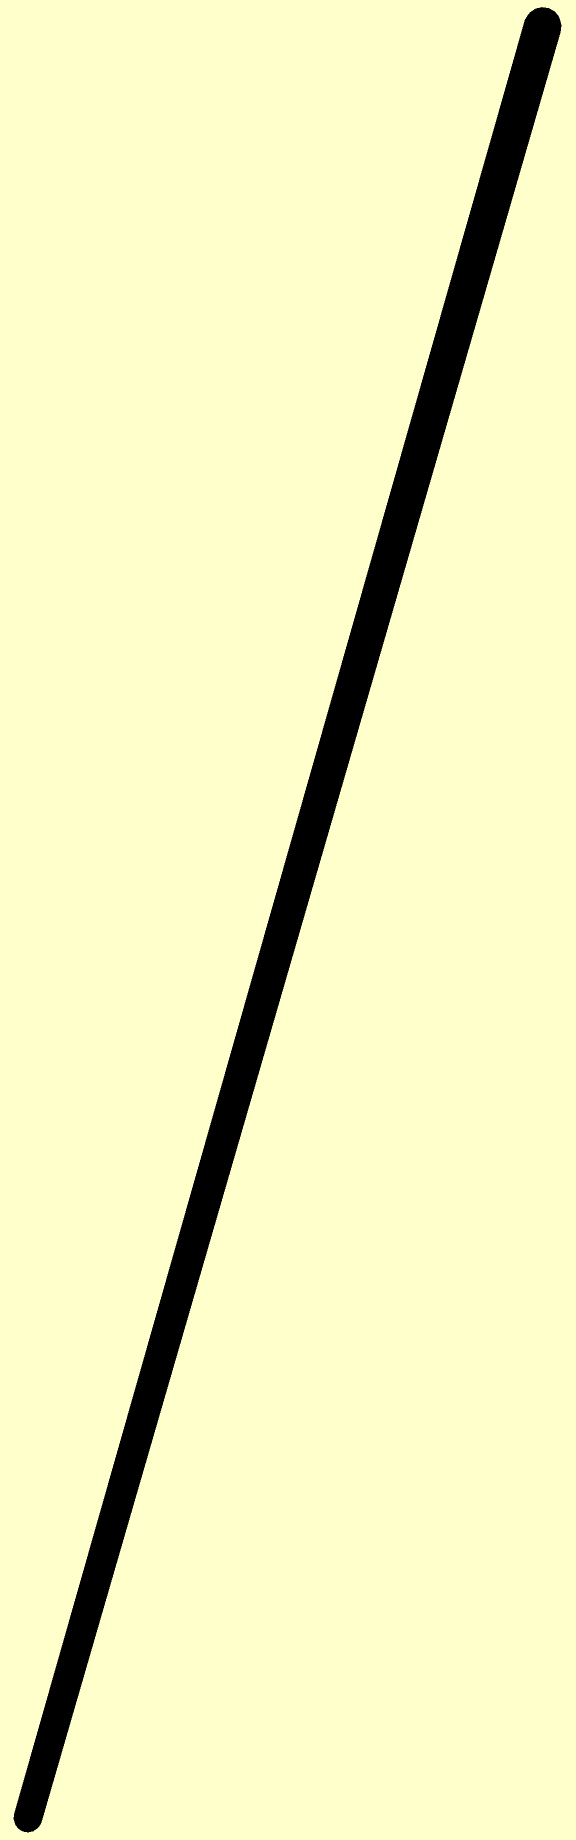
\includegraphics{anti_aliasing-highres.png}};
		\spy [blue] on (highrespng.center)
						in node[above, yshift=0.1cm] at (highrespng.north);
	\end{scope}
	\makeresolutionnode{highrespng}
	
	\begin{scope}[my spy]
		\node[anchor=south west,inner sep=0] (truehighres) [right=of highrespng] {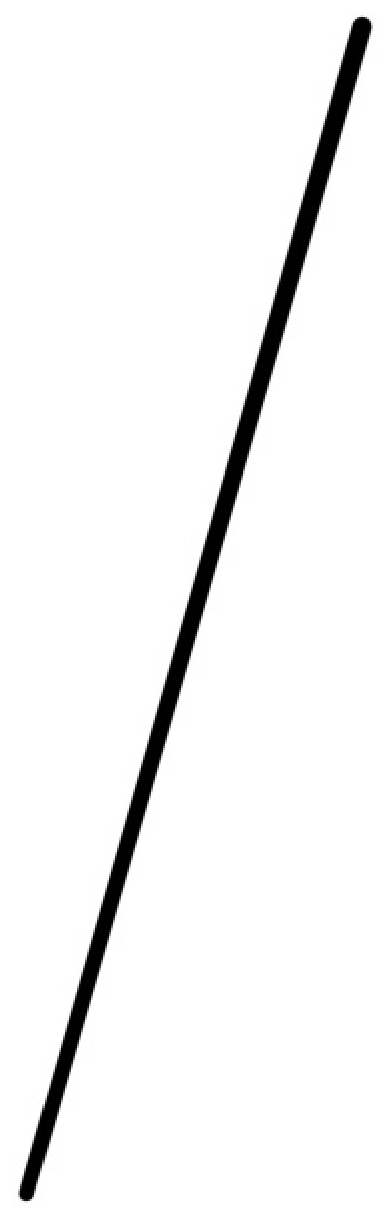
\includegraphics[scale=0.25]{anti_aliasing-truehighres.pdf}};
		\spy [blue] on (truehighres.center)
						in node[above, yshift=0.1cm] at (truehighres.north|-highrespng.north);
	\end{scope}
	\node[level text] at (highrespng label -| truehighres.center) {\makeresolutionlabel{subfig:truehighres}};
		
	\begin{scope}[my spy]
		\node[anchor=south west, inner sep=0] (frameonly) [right=of truehighres] {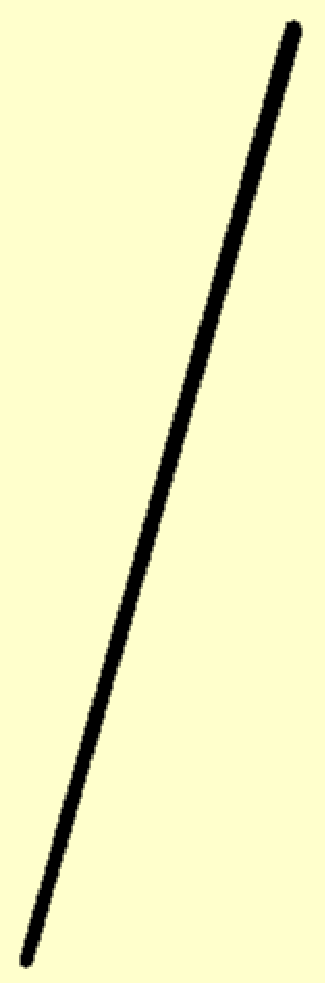
\includegraphics[scale=0.25]{anti_aliasing-frameonly.pdf}};
		\spy [blue] on (frameonly.center)
						in node[above, yshift=0.1cm] at (frameonly.north|-lowres.north);
	\end{scope}
	\node[level text] at (highrespng label -| frameonly.center) {\makeresolutionlabel{subfig:frameonly}};
\end{tikzpicture}
\end{center}

\setlength{\emergencystretch}{1em}\par
\noindent There are (at least) two ways to improve the actual resolution beyond the 
apparent ``limit'' illustrated in \ref{subfig:highrespdf}.

\setlength{\emergencystretch}{0em}
\begin{enumerate}
\item Changing the format from \verb+pdf+ to the format \verb+png+, which is used for 
rasterized images, will cause high values of \lstinline!settings.render! to produce high-resolution 
images, as seen in \ref{subfig:highrespng}. This is the simpler method, and usually the recommended one. 
The main drawback to this method is that with a \verb+png+ file, any two-dimensional parts 
to the image
will be rasterized as well.  Thus, this method is not ideal for producing images with mixed two- and 
three-dimensional output, such as the one on 
page~\pageref{figure:target_diagram}.
\item Alternatively, adding the line 
\begin{lstlisting}
shipout(scale(4.0)*currentpicture.fit());
\end{lstlisting}
 to the 
end of the code will cause the entire Asymptote picture (including any text) to be scaled up by a 
factor of \lstinline!4.0!. (Other factors can, of course, be substituted.)  This increases the threshold 
for higher values of \lstinline!settings.render! to produce better results, as seen in 
\ref{subfig:truehighres}. [Note that scaling up the image without increasing \lstinline!settings.render! 
does not do any good, as seen in \ref{subfig:frameonly}.]  The main disadvantage of 
this method, aside from its complexity, is that the resulting image must be scaled back down.  Thus, 
for instance, \ref{subfig:truehighres} and \ref{subfig:frameonly} 
were each included in a \verb+.tex+ file using the 
line \verb+\includegraphics[scale=0.25]{filename.pdf}+ (with \lstinline!filename! replaced by 
the actual file name).  It would also have worked in this case to replace \lstinline![scale=0.25]! by 
\lstinline![width=1.2cm]!; this is, in fact, the only viable option for producing high-resolution 
rasterized images with the Asymptote code written into a \LaTeX{} file via the \verb+asymptote+ package.

A second disadvantage is that this method can make small changes to the dimensions of the 
resulting picture; in the images above, the two rightmost images are both taller and wider than 
the preceeding four images.  This is unlikely to cause problems as long as you are consistent in 
which method you use.
\end{enumerate}

\noindent Here is the code that was used to produce the images above.  
The lines of code under discussion are in red.

\def\currentlistingwidth{0.48\linewidth}
\lstset{moredelim=[is][\color{red}]{|}{|}}
\medskip\noindent
\begin{minipage}{\currentlistingwidth}
\ref{subfig:lowres}
\begin{lstlisting}
settings.outformat="pdf";
|settings.render=1;|
settings.prc = false;
import three;
size(1cm,0);
draw((0,0,0) -- (1,1,1), linewidth(2pt));
\end{lstlisting}
\end{minipage}
\hfill
\begin{minipage}{\currentlistingwidth}
\ref{subfig:medres}
\begin{lstlisting}
settings.outformat="pdf";
|settings.render=4;|
settings.prc = false;
import three;
size(1cm,0);
draw((0,0,0) -- (1,1,1), linewidth(2pt));
\end{lstlisting}
\end{minipage}
\begin{minipage}{\currentlistingwidth}
\ref{subfig:highrespdf}
\begin{lstlisting}
settings.outformat="pdf";
|settings.render=16;|
settings.prc = false;
import three;
size(1cm,0);
draw((0,0,0) -- (1,1,1), linewidth(2pt));
\end{lstlisting}
\end{minipage}
\hfill
\begin{minipage}{\currentlistingwidth}
\ref{subfig:highrespng}
\begin{lstlisting}
|settings.outformat="png";|
|settings.render=16;|

import three;
size(1cm,0);
draw((0,0,0) -- (1,1,1), linewidth(2pt));
\end{lstlisting}
\end{minipage}
\begin{minipage}{\currentlistingwidth}
\ref{subfig:truehighres}
\begin{lstlisting}
settings.outformat="pdf";
|settings.render=16;|
settings.prc = false;
import three;
size(1cm,0);
draw((0,0,0) -- (1,1,1), linewidth(2pt));
|shipout(scale(4.0) * currentpicture.fit());|
\end{lstlisting}
\end{minipage}
\hfill
\begin{minipage}{\currentlistingwidth}
\ref{subfig:frameonly}
\begin{lstlisting}
settings.outformat="pdf";

settings.prc = false;
import three;
size(1cm,0);
draw((0,0,0) -- (1,1,1), linewidth(2pt));
|shipout(scale(4.0) * currentpicture.fit());|
\end{lstlisting}
\end{minipage}

\subsection{Three-dimensional paths}
The built-in type for a three-dimensional path in Asymptote is \lstinline!path3!\index{path3@\texttt{path3}}. 
An intermediate type is \lstinline!guide3!\index{guide3@\texttt{guide3}}; functions will often return 
a \lstinline!guide3! when you want a \lstinline!path3!, but this is fine since Asymptote can automatically 
convert the former to 
the latter.  
Much as in the case of two-dimensional paths, the \lstinline!--! operator connects two points 
by a line segment, while \lstinline!..! uses a smooth curve.  Either can be followed by the another, already 
constructed path or by the keyword \lstinline!cycle!, which closes the curve.  
Another useful function 
is \lstinline!dot(triple)!\index{dot@\texttt{dot()}}, which draws a small sphere at the indicated point; in 
the following code, this is used together with the pen lift operator \lstinline!^^! to dot several 
points in one fell swoop.

\begin{asyexample}{4.3cm}
\begin{asypicture}{}
settings.outformat="png";
settings.render=8;
import three;
size(4cm,0);
draw(-X -- X .. Y .. X-Y+Z .. cycle);
dot(-X ^^ X ^^ Y ^^ X-Y+Z);
finish();
\end{asypicture}
\begincodelisting
\begin{lstlisting}
settings.outformat="png";
settings.render=8;
import three;
size(4cm,0);
draw(-X -- X .. Y .. X-Y+Z .. cycle);
dot(-X ^^ X ^^ Y ^^ X-Y+Z);
\end{lstlisting}
\end{asyexample}

Another interesting operator is \lstinline!---!.  Like the operator \lstinline!--!, it draws a line segment 
between two points; unlike that operator, it tries to keep the path smooth beyond those two points if possible.
Note that this operator works in the two-dimensional context also.

\begin{asyexample}{4.3cm}
\begin{asypicture}{}
settings.outformat="png";
settings.render=8;
import three;
size(4cm,0);
draw(-X --- X .. Y .. X-Y+Z .. cycle);
dot(-X ^^ X ^^ Y ^^ X-Y+Z);
finish();
\end{asypicture}
\begincodelisting
\begin{lstlisting}
settings.outformat="png";
settings.render=8;
import three;
size(4cm,0);
draw(-X --- X .. Y .. X-Y+Z .. cycle);
dot(-X ^^ X ^^ Y ^^ X-Y+Z);
\end{lstlisting}
\end{asyexample}

\subsubsection{Parallelograms and 3d boxes}
To draw the outline of a parallelogram with sides given by the vectors \lstinline!u! and \lstinline!v! 
starting at the point \lstinline!O!, use the function
\begin{lstlisting}
path3 plane(triple u, triple v, triple O=O);
\end{lstlisting}
Here's an example:

\begin{asyexample}{4.3cm}
\begin{asypicture}{}
settings.outformat="png";
settings.render=16;
import three;
size(4cm,0);
draw(O--2X ^^ O--2Y ^^ O--2Z, black);
draw(plane(O=X, Y-X, Z-X), blue);
finish();
\end{asypicture}
\begincodelisting
\begin{lstlisting}
settings.outformat="png";
settings.render=16;
import three;
size(4cm,0);
draw(O--2X ^^ O--2Y ^^ O--2Z, black);
draw(plane(O=X, Y-X, Z-X), blue);
\end{lstlisting}
\end{asyexample}
\noindent
Somewhat confusingly, a parameter named \lstinline!O! need not have the value \lstinline!O=(0,0,0)!, 
although that is its default value.

To draw the outline of a rectangular solid with opposite vertices at \lstinline!v1! and \lstinline!v2!, 
use the function
\begin{lstlisting}
path3[] box(triple v2, triple v2);
\end{lstlisting}
Here's an example:

\begin{asyexample}{4.3cm}
\begin{asypicture}{}
settings.outformat="png";
settings.render=16;
import three;
size(4cm,0);
draw(O--2X ^^ O--2Y ^^ O--2Z);
draw(box(O, (0.5, 1.5, 1)), blue);
finish();
\end{asypicture}
\begincodelisting
\begin{lstlisting}
settings.outformat="png";
settings.render=16;
import three;
size(4cm,0);
draw(O--2X ^^ O--2Y ^^ O--2Z);
draw(box(O, (0.5, 1.5, 1)), blue);
\end{lstlisting}
\end{asyexample}

\subsubsection{Circles and arcs}
The function
\begin{lstlisting}
path3 circle(triple c, real r, triple normal=Z);
\end{lstlisting}
creates an approximate circle in three-dimensional space with center \lstinline!c! and
radius \lstinline!r! that lies in the plane normal to \lstinline!normal!:

\needspace{11\baselineskip}
\begin{asyexample}{4.3cm}
\begin{asypicture}{}
settings.outformat="png";
settings.render=16;
import three;
size(4cm,0);
draw(O--2X ^^ O--2Y ^^ O--2Z);
triple circleCenter = (Y+Z)/sqrt(2) + X;
path3 mycircle = circle(c=circleCenter, r=1, normal=Y+Z);
draw(plane(O=sqrt(2)*Z, 2X, 2*unit(Y-Z)), gray + 0.1cyan);
draw(mycircle, blue);
draw(shift(circleCenter) * (O -- Y+Z), green, arrow=Arrow3());
finish();
\end{asypicture}
\begincodelisting
\begin{lstlisting}
settings.outformat="png";
settings.render=16;
import three;
size(4cm,0);
draw(O--2X ^^ O--2Y ^^ O--2Z);
triple circleCenter = (Y+Z)/sqrt(2) + X;
path3 mycircle = circle(c=circleCenter, r=1, normal=Y+Z);
\end{lstlisting}
\breakcodelisting
\begin{lstlisting}
draw(plane(O=sqrt(2)*Z, 2X, 2*unit(Y-Z)), gray + 0.1cyan);
draw(mycircle, blue);
draw(shift(circleCenter) * (O -- Y+Z), green, arrow=Arrow3());
\end{lstlisting}
\end{asyexample}

The most convenient function to create arcs in three dimensions is 
\begin{lstlisting}
path3 arc(triple c, triple v1, triple v2, triple normal=O);
\end{lstlisting}
which draws an arc centered at \lstinline!c! from \lstinline!v1! to the line through \lstinline!c! 
and \lstinline!v2!.  By default, the arc drawn will be $\leq 180^{\circ}$.  If it is exactly $180^{\circ}$---i.e., if \lstinline!v1!, \lstinline!v2!, and \lstinline!c! are 
all collinear---then the normal is necessary to determine the plane of the arc.  Otherwise, the normal vector 
is optional, but can be used to force the complementary arc (greater than $180^{\circ}$).

\begin{asyexample}{4.3cm}
\begin{asypicture}{}
settings.outformat="png";
settings.render=16;
import three;
size(4cm);

draw(-2X--2X, arrow=Arrow3(emissive(black)));
draw(-2Y--2Y, arrow=Arrow3(emissive(black)));
draw(-2Z--2Z, arrow=Arrow3(emissive(black)));
draw(path3(box((-2,-2),(2,2))), gray);
draw(arc(c=O, Y, Z), blue, arrow = Arrow3(TeXHead2, emissive(blue)));
draw(arc(c=O, -Y, Z), blue, arrow = Arrow3(TeXHead2, emissive(blue)));
draw(arc(c=(1,1,0), Y, 2X, normal=Z), green, arrow = Arrow3(TeXHead2(normal=Z), emissive(green)));
draw(arc(c=(1,1,0), Y, 2X, normal=-Z), red, arrow = Arrow3(TeXHead2(normal=Z), emissive(red)));
finish();
\end{asypicture}
\begincodelisting
\begin{lstlisting}[escapechar=!]
settings.outformat="png";
settings.render=16;
import three;
size(4cm);

draw(-2X--2X, arrow=Arrow3(emissive(black)));
!\quad!
\end{lstlisting}
\breakcodelisting
\begin{lstlisting}[escapechar=\%]
draw(-2Y--2Y, arrow=Arrow3(emissive(black)));
draw(-2Z--2Z, arrow=Arrow3(emissive(black)));%\pagebreak[1]%
draw(path3(box((-2,-2),(2,2))), gray);
draw(arc(c=O, Y, Z), blue, arrow = Arrow3(TeXHead2, emissive(blue)));
draw(arc(c=O, -Y, Z), blue, arrow = Arrow3(TeXHead2, emissive(blue)));
draw(arc(c=(1,1,0), Y, 2X, normal=Z), green, arrow = Arrow3(TeXHead2(normal=Z), emissive(green)));
draw(arc(c=(1,1,0), Y, 2X, normal=-Z), red, arrow = Arrow3(TeXHead2(normal=Z), emissive(red)));
\end{lstlisting}
\end{asyexample}

\subsubsection{Planar curves}
To convert a two-dimensional \verb|path| variable into a three-dimensional \verb|path3|, use the 
function
\begin{lstlisting}
path3 path3(path p, triple plane(pair) = XYplane);
\end{lstlisting}
By default, this function treats maps the path into the $xy$-plane by applying $(x,y) \mapsto (x,y,0)$. 
If the optional argument is changed to \verb|ZXplane| or \verb|YZplane|, then 
$(x,y)$ maps to $(y,0,x)$ or $(0,x,y)$, respectively.

\begin{asyexample}{4.3cm}
\begin{asypicture}{name=planar_curve}
settings.outformat = "png";
settings.render=16;
import three;
size(@mywidth - 0.15cm, 0);

path p = box((0,-0), (3,1));
draw(path3(p), black);
draw(path3(p, plane=ZXplane), blue);
draw(path3(p, plane=YZplane), red);

finish();
\end{asypicture}
\begincodelisting
\begin{lstlisting}
settings.outformat = "png";
settings.render=16;
import three;
size(4.15cm, 0);

path p = box((0,-0), (3,1));
draw(path3(p), black);
draw(path3(p, plane=ZXplane), blue);
draw(path3(p, plane=YZplane), red);
\end{lstlisting}
\end{asyexample}

Janet can use this to start lifting her two-dimensional diagram to three
dimensions:

\begin{asyexample}{4.3cm}
\begin{asypicture}{name=axesonside}
//Basic settings
settings.outformat = "png";
settings.render = 8;
import graph;
import three;
size(4.15 cm, 0);

//Save some important numbers.
real xmin = -0.1;
real xmax = 2;
real ymin = -0.1;
real ymax = 2;

//Construct the graph.
real f(real x) { return sqrt(x); }
path s = graph(f, 0, 2, operator..);

//Draw the graph and the axes.
draw(path3(s));
draw(xmin*X -- xmax*X);
draw(ymin*Y -- ymax*Y);

finish();
\end{asypicture}
\begincodelisting
\lstinputlisting[firstline=18, lastline=21]{\jobname-axesonside.asy}
\breakcodelisting
\lstinputlisting[firstline=22, lastline=38]{\jobname-axesonside.asy}
\end{asyexample}
\noindent
She is dissatisfied with the result, since the axes are lying down in 
a horizontal plane rather than standing upright. This will be corrected
later, by playing with the point of view---specifically the \lstinline!up!
parameter, which controls which way is up.

\subsubsection{Parametric curves}
For drawing complicated three-dimensional curves in Asymptote, assembling them point-by-point is not 
generally feasible.  Instead, it is better to describe the curve by a parametric function and then plot it using 
the \verb|graph| function from the \verb|graph3| module:

\begin{asyexample}{4.3cm}
\begin{asypicture}{name=parametric_curve}
settings.outformat="png";
settings.render=16;
import graph3;
size(@mywidth-.15cm, 0);
currentprojection = orthographic(0,2,1);

triple f(real t) {
    return (t*cos(t), t*sin(t), t);
}

path3 spiral = graph(f, 0, 8pi, operator ..);
draw(spiral);
finish();
\end{asypicture}
\begincodelisting
\begin{lstlisting}[escapechar=!]
settings.outformat="png";
settings.render=16;
import graph3;
size(4.15cm, 0);
currentprojection = orthographic(0,2,1);
!\quad!
\end{lstlisting}
\breakcodelisting
\begin{lstlisting}
triple f(real t) {
    return (t*cos(t), t*sin(t), t);
}

path3 spiral = graph(f, 0, 8pi, operator ..);
draw(spiral);
\end{lstlisting}
\end{asyexample}

\subsection{Surfaces of revolution}
\label{subsection:revolution}

The most interesting surface Janet needs to draw is not a sphere, but a surface obtained by revolving 
the graph of $y=\sqrt{x}$ about the $x$-axis.
She is prepared to work out how to define it as a parametric surface, but is gratified to learn 
that there is a simpler way: Asymptote has a facility for producing surfaces of revolution directly.

\medskip
\begin{danger}
The \lstinline!surface()! function that I am about to introduce to create surfaces of revolution 
is undocumented.  Thus, it could conceivably
cease to work without notice in future versions of Asymptote.  If this should happen, it should 
still be possible to create surfaces of revolution in a slightly longer way using the \lstinline!solids! 
module, which is documented.
\end{danger}
\medskip

The documentation recommends creating surfaces of revolution using functions from the 
module \lstinline!solids!, which allows additional options such as drawing silhouettes.  However, 
if all you want to do is create a surface of revolution (with no silhouettes, skeletons, etc.), then 
the following function from the module \lstinline!three! is typically simpler to use. 
The function is defined in the file \lstinline!three_surface.asy!, which is automatically included 
when the \lstinline!three! module is loaded.  Here is the specification\footnote{This is a special 
kind of function called a \emph{constructor}. Its return type is the same as its name, in this case 
\lstinline!surface!.} of the function, including only the 
required parameters:
%// Construct the surface of rotation generated by rotating g
%// from angle1 to angle2 sampled n times about the line c--c+axis.
%// An optional surface pen color(int i, real j) may be specified
%// to override the color at vertex(i,j).
%void operator init(triple c, path3 g, triple axis, int n=nslice,
%                     real angle1=0, real angle2=360,
%                     pen color(int i, real j)=null) 
\begin{lstlisting}
surface(triple c, path3 g, triple axis);
\end{lstlisting}
The type \lstinline!triple!, as discussed earlier, represents an ordered triple $(a,b,c)$; depending 
on context, this can be a point or a vector in three-dimensional space $\mathbb{R}^3$.  The type 
\lstinline!path3!\index{path3@\texttt{path3}} represents a path in three dimensions; objects of this 
type behave very similarly to paths in two dimensions (of type \lstinline!path!).  In particular, a
line segment in three dimensions like \lstinline!O -- 2X! is an object of type \lstinline!path!.

The effect of this function is to revolve the path \lstinline!g! about the line \lstinline!c -- c+axis!, i.e., 
the line through the point $c$ in the direction $\vec{axis}$,  and return the resulting surface of revolution. 
The surface may then be drawn with the \lstinline!draw()! function.

\begin{asyexample}{5.3cm}
\begin{asypicture}{}
settings.outformat="png";
settings.render=8;
import three;

size(5cm,0);
//create segment
path3 segment = (0,1.2,0) -- (0,0.6,1.5);
//create surface of revolution
surface lampshade = surface(segment, c=O, axis=Z);
//draw surface
draw(lampshade, yellow);
//draw revolved segment for reference
draw(segment, black);
//draw axes for reference
draw(O--2X, blue); //x-axis
draw(O--2Y, green); //y-axis
draw(O--2Z, red); //z-axis
finish();
\end{asypicture}
\begincodelisting
\begin{lstlisting}
settings.outformat="png";
settings.render=8;
import three;

size(5cm,0);
//create segment
path3 segment = (0,1.2,0) -- (0,0.6,1.5);
//create surface of revolution
surface lampshade = surface(segment, c=O, axis=Z);
\end{lstlisting}
\breakcodelisting
\begin{lstlisting}[escapechar=\%]
//draw surface%\pagebreak[0]%
draw(lampshade, yellow);%\pagebreak[1]%
//draw revolved segment for reference
draw(segment, black);
//draw axes for reference
draw(O--2X, blue); //x-axis
draw(O--2Y, green); //y-axis
draw(O--2Z, red); //z-axis
\end{lstlisting}
\end{asyexample}

Here's a first stab at using this to construct the surface of revolution
in Janet's diagram. (Recall that \lstinline!s! was the name of the
two-dimensional graph of $y=\sqrt{x}$.)

\begin{asyexample}{4.3cm}
\begin{asypicture}{name=janetsurfaceofrotation}
//Basic settings
settings.outformat = "png";
settings.render = 8;
defaultpen(fontsize(10pt));
import graph;
import three;
size(4.15 cm, 0);

//Save some important numbers.
real xmin = -0.1;
real xmax = 2;
real ymin = -0.1;
real ymax = 2;

//Construct the graph.
real f(real x) { return sqrt(x); }
path s = graph(f, 0, 2, operator..);

//Draw the graph and the axes.
path3 p3 = path3(s);
draw(p3);
/*red*/surface solidsurface = surface(p3, c=O, axis=X);
draw(solidsurface, white);/*red*/
draw(xmin*X -- xmax*X);
draw(ymin*Y -- ymax*Y);

finish();
\end{asypicture}
\begincodelisting
\begin{lstlisting}[escapechar=!,belowskip=0pt]
!\quad!
!\qquad\smash{\raisebox{1ex}{\vdots}}!
\end{lstlisting}\lstset{moredelim=[is][\color{red}]{/*red*/}{/*red*/}}
\lstinputlisting[aboveskip=0pt,firstline=37,lastline=42]{\asylistingfile}
\end{asyexample}

\subsubsection{optional parameters}
Since this function seems to be undocumented, here are the optional parameters, 
as defined by the source code, together with Vincent's best guesses about what they mean.
\begin{center}
\begin{tabular}{@{} l l l @{}}						\toprule
type			& name			& default value		\\ \midrule
\verb'int'		& \verb'n'			& \verb'nslice' (usually 12)		\\ 
\verb'real'		& \verb'angle1'		& \verb'0'			\\
\verb'real'		& \verb'angle2'		& \verb'360'		\\
\verb'pen(int,real)'	& \verb'color'	& \verb'null'		\\ \bottomrule
\end{tabular}
\end{center}
The function creates a surface by revolving the given path
from \verb|angle1| 
to \verb|angle2| (in degrees) about the specified axis.  The parameter \verb|n| can be used to 
refine the mesh, making the surface more accurate (for higher values of \verb|n|) or 
faster to produce and draw (for lower values of \verb|n|).

The parameter \verb|color()| is a function that can be used to vary color within the surface, 
overriding any color parameter passed to the \verb|draw()| command when applied to 
the surface.
The first parameter of \verb|color()| represents distance along the path (in the sense of 
``path times''), while the second parameter represents the number of slices of the revolution.

Here's an example that uses all of these optional parameters:

\begin{center}
\begin{asypicture}{name=colored_torus, width = \linewidth}
settings.outformat = "png";
settings.render=16;
size(@the@linewidth,0);
import graph3;
currentprojection = perspective(30*dir(75,0));
real r1=5, r0=1;
int nu = 36, nv = 36;
path3 crossSection = Circle(r=r0, c=(r1,0,0), normal=Y, n= nu);
pen colorFunction(int u, real theta) {
    real z = sin(u/nu * 2pi);
    real t = (z + 1) / 2;
    return t*red + (1-t)*lightblue;
}
surface torus = surface(crossSection, c=(0,0,0), axis=Z, n=nv, angle1=90, angle2=410, color=colorFunction);
draw(torus);
finish();
\end{asypicture}
\begin{lstlisting}
settings.outformat = "png";
settings.render=16;
size(345.0pt,0);
import graph3;
currentprojection = perspective(30*dir(75,0));
real r1=5, r0=1;
int nu = 36, nv = 36;
path3 crossSection = Circle(r=r0, c=(r1,0,0), normal=Y, n= nu);
pen colorFunction(int u, real theta) {
    real z = sin(u/nu * 2pi);
    real t = (z + 1) / 2;
    return t*red + (1-t)*lightblue;
}
surface torus = surface(crossSection, c=(0,0,0), axis=Z, n=nv, angle1=90, angle2=410, color=colorFunction);
draw(torus);
\end{lstlisting}
\end{center}


\subsection{Points of view; projections}
For non-interactive images, choosing a good point of view is something of an art. 
The way to select a point of view in Asymptote is to set the value of the predefined variable 
\lstinline!currentprojection!, of type \lstinline!projection!.  Here are the most relevant options:
%
\subsubsection{Oblique projection}
Janet is used to a very simple setup for drawing three-dimensional objects on a two-dimensional 
chalkboard (or paper): the $x$ and $y$ axes are drawn as usual, and the $z$ axis is drawn pointing 
down and to the left with a slope of $1$.  The $z$-axis is supposed to be imagined 
as sticking out of the page.  This setup is especially nice for drawing surfaces of revolution 
on the board, since one can draw the curve exactly as usual in the $xy$-plane and then talk about 
revolving it about the $x$ or $y$ axis.

Asymptote does support this setup: it is called an oblique projection. 
Unfortunately, this surface of revolution
about the $y$-axis looks much stranger here than it does on the chalkboard:
%
\begin{asyexample}{5.3cm}
\begin{asypicture}{}
settings.outformat="png";
settings.render=8;
defaultpen(fontsize(10pt));
import three;
size(5cm,0);
currentprojection = oblique;
draw(O -- 2X, L=Label("$x$", position=EndPoint));
draw(O -- 3.5Y, L=Label("$y$", position=EndPoint));
draw(O -- 2Z, L=Label("$z$", position=EndPoint));
draw(box(O, (1,1.5,1.25)), blue+linewidth(0.6pt));
draw(surface(2Y -- 3Y+X, c=O, axis=Y), yellow);
finish();
\end{asypicture}
\begincodelisting
\begin{lstlisting}
settings.outformat="png";
settings.render=8;
defaultpen(fontsize(10pt));
import three;
size(5cm,0);
|currentprojection = oblique;|
draw(O -- 2X, L=Label("$x$", position=EndPoint));
draw(O -- 3.5Y, L=Label("$y$", position=EndPoint));
draw(O -- 2Z, L=Label("$z$", position=EndPoint));
draw(box(O, (1,1.5,1.25)), blue+linewidth(0.6pt));
draw(surface(2Y -- 3Y+X, c=O, axis=Y), yellow);
\end{lstlisting}
\end{asyexample}
\noindent
Janet wonders if this is a bug in Asymptote.  Vincent does some research and finds out that 
the problem is something inherent in the oblique projection: fundamentally, it is an unrealistic 
simplification of the projection of three-dimensional space onto a two-dimensional plane.  For some 
objects it looks okay, but some things---especially surfaces of revolution (including some 
arrowheads in Asymptote)---just look weird.

In spite of the weirdness visible here, oblique projections are occasionally useful, so it is 
worthwhile to note that Asymptote also has projections called \lstinline!obliqueX! and \lstinline!obliqueY!, 
with the $x$ and $y$ axes (respectively) sticking ``out of the page.''  The \lstinline!obliqueZ! projection 
is the same as just plain \lstinline!oblique!.
\begin{asyexample}{5.3cm}
\begin{asypicture}{}
settings.outformat="png";
settings.render=8;
defaultpen(fontsize(10pt));
import three;
size(5cm,0);
currentprojection = obliqueX;
draw(O -- 2X, L=Label("$x$", position=EndPoint));
draw(O -- 3.5Y, L=Label("$y$", position=EndPoint));
draw(O -- 2Z, L=Label("$z$", position=EndPoint));
draw(box(O, (1,1.5,1.25)), blue+linewidth(0.6pt));
draw(surface(2Y -- 3Y+X, c=O, axis=Y), yellow);
finish();
\end{asypicture}
\begincodelisting
\begin{lstlisting}[escapechar=!]
!\quad!
!\qquad\smash{\raisebox{1ex}{\vdots}}!
currentprojection = obliqueX;
!\quad!
!\qquad\smash{\raisebox{1ex}{\vdots}}!
\end{lstlisting}
\end{asyexample}
%
\subsubsection{Perspective}
On the other end of the spectrum lies vanishing point perspective, which is ``realistic": closer 
objects appear larger.  The line 
\begin{lstlisting}
currentprojection = perspective(5,2,3);
\end{lstlisting}
tells Asymptote to draw the image as though it were produced by a camera located at the point $(5,2,3)$.
The following three images show the same scene in perspective as the camera moves farther and 
farther away  from the origin.  Note that in the first image especially, text that is closer to the camera 
is visibly larger than text that is farther away. If this behavior is 
undesired, it can be prevented by including the two lines
\lstinline!Embedded.targetsize = true; Billboard.targetsize = true;! after
the imports, although this will look funny if an interactive view is desired.
\begin{asyexample}{5.4cm}
\begin{asypicture}{}
settings.outformat="png";
settings.render=16;
defaultpen(fontsize(10pt));
import three;
size(5cm,0);
currentprojection = perspective(5,2,3);
draw(O -- 2X, L=Label("$x$", position=EndPoint));
draw(O -- 3.5Y, L=Label("$y$", position=EndPoint));
draw(O -- 2Z, L=Label("$z$", position=EndPoint));
draw(box(O, (1,1.5,1.25)), blue+linewidth(0.6pt));
draw(surface(2Y -- 3Y+X, c=O, axis=Y), yellow);
finish();
\end{asypicture}
\begincodelisting
\begin{lstlisting}
settings.outformat="png";
settings.render=16;
defaultpen(fontsize(10pt));
import three;
size(5cm,0);
|currentprojection = perspective(5,2,3);|
draw(O -- 2X, L=Label("$x$", position=EndPoint));
draw(O -- 3.5Y, L=Label("$y$", position=EndPoint));
\end{lstlisting}
\breakcodelisting
\begin{lstlisting}[escapechar=\%]
draw(O -- 2Z, L=Label("$z$", position=EndPoint));
draw(box(O, (1,1.5,1.25)), blue+linewidth(0.6pt));%\pagebreak[1]%
draw(surface(2Y -- 3Y+X, c=O, axis=Y), yellow);
\end{lstlisting}
\end{asyexample}
%
\begin{asyexample}{5.4cm}
\begin{asypicture}{}
settings.outformat="png";
settings.render=8;
defaultpen(fontsize(10pt));
import three;
size(5cm,0);
currentprojection = perspective(2*(5,2,3));
draw(O -- 2X, L=Label("$x$", position=EndPoint));
draw(O -- 3.5Y, L=Label("$y$", position=EndPoint));
draw(O -- 2Z, L=Label("$z$", position=EndPoint));
draw(box(O, (1,1.5,1.25)), blue+linewidth(0.6pt));
draw(surface(2Y -- 3Y+X, c=O, axis=Y), yellow);
finish();
\end{asypicture}
\begincodelisting
\begin{lstlisting}[escapechar=!]
!\strut!
!\raisedvdots!
currentprojection = perspective(2*(5,2,3));
!\strut!
!\raisedvdots!
\end{lstlisting}
\end{asyexample}
%
\begin{asyexample}{5.4cm}
\begin{asypicture}{}
settings.outformat="png";
settings.render=8;
defaultpen(fontsize(10pt));
import three;
size(5cm,0);
currentprojection = perspective(4*(5,2,3));
draw(O -- 2X, L=Label("$x$", position=EndPoint));
draw(O -- 3.5Y, L=Label("$y$", position=EndPoint));
draw(O -- 2Z, L=Label("$z$", position=EndPoint));
draw(box(O, (1,1.5,1.25)), blue+linewidth(0.6pt));
draw(surface(2Y -- 3Y+X, c=O, axis=Y), yellow);
finish();
\end{asypicture}
\begincodelisting
\begin{lstlisting}[escapechar=!]
!\strut!
!\raisedvdots!
currentprojection = perspective(4*(5,2,3));
!\strut!
!\raisedvdots!
\end{lstlisting}
\end{asyexample}

\noindent
The optional argument \lstinline!up=triple! tells Asymptote to rotate the camera (without changing 
where it is pointing) so that the  specified vector will appear to point up:
%
\begin{asyexample}{4.3cm}
\begin{asypicture}{}
settings.outformat="png";
settings.render=8;
settings.prc=false;
defaultpen(fontsize(10pt));

import three;
size(4cm,0);

currentprojection = perspective(3*(5,2,3), up=Y);

draw(O -- 2X, L=Label("$x$", position=EndPoint));
draw(O -- 3.5Y, L=Label("$y$", position=EndPoint));
draw(O -- 2Z, L=Label("$z$", position=EndPoint));

draw(box(O, (1,1.5,1.25)), blue+linewidth(0.6pt));

draw(surface(2Y -- 3Y+X, c=O, axis=Y), yellow);
finish();
\end{asypicture}
\begincodelisting
\begin{lstlisting}[escapechar=!]

!\raisedvdots!
size(4cm,0);
currentprojection = perspective(3*(5,2,3), up=Y);

!\raisedvdots!
\end{lstlisting}
\end{asyexample}

One of the features Janet wants is that the $x$-axis should appear exactly horizontal and the $y$-axis 
exactly vertical.  
Theoretically, 
modifying the previous example to put the camera in the $xz$-plane while keeping \lstinline!up=Y! 
ought to do this.
%
\begin{asyexample}{4.3cm}
\begin{asypicture}{}
settings.outformat="png";
settings.render=8;
settings.prc=false;
defaultpen(fontsize(10pt));

import three;
size(4cm,0);

currentprojection = perspective(3*(5,0,3), up=Y);

draw(O -- 2X, L=Label("$x$", position=EndPoint));
draw(O -- 3.5Y, L=Label("$y$", position=EndPoint));
draw(O -- 2Z, L=Label("$z$", position=EndPoint));

draw(box(O, (1,1.5,1.25)), blue+linewidth(0.6pt));

draw(surface(2Y -- 3Y+X, c=O, axis=Y), yellow);
finish();
\end{asypicture}
\begincodelisting
\begin{lstlisting}[escapechar=!]

!\raisedvdots!
currentprojection = perspective(3*(5,0,3), up=Y);

!\raisedvdots!
\end{lstlisting}
\end{asyexample}
\noindent
This basically works, but the effect is slightly spoiled when the axes appear to get bigger as they grow 
closer.


%
\subsubsection{Orthographic projection}
After the line
\begin{lstlisting}
currentprojection=orthographic((5,2,3));
\end{lstlisting}
the image is drawn as if it were a zoomed-in picture taken by a camera very far away in the direction 
of the vector $(5,2,3)$:
%
\begin{asyexample}{5.3cm}
\begin{asypicture}{}
settings.outformat="png";
settings.render=8;
settings.prc=false;
defaultpen(fontsize(10pt));

import three;
size(5cm,0);

currentprojection = orthographic((5,2,3));

draw(O -- 2X, L=Label("$x$", position=EndPoint));
draw(O -- 3.5Y, L=Label("$y$", position=EndPoint));
draw(O -- 2Z, L=Label("$z$", position=EndPoint));

draw(box(O, (1,1.5,1.25)), blue+linewidth(0.6pt));

draw(surface(2Y -- 3Y+X, c=O, axis=Y), yellow);
finish();
\end{asypicture}
\begincodelisting
\begin{lstlisting}[escapechar=!]
settings.outformat="png";
settings.render=4;
defaultpen(fontsize(10pt));
import three;
size(5cm,0);
|currentprojection = orthographic((5,2,3));|
draw(O -- 2X, L=Label("$x$", position=EndPoint));
!\strut!
\end{lstlisting}
\breakcodelisting
\begin{lstlisting}[escapechar=\%]
draw(O -- 3.5Y, L=Label("$y$", position=EndPoint));%\pagebreak[1]%
draw(O -- 2Z, L=Label("$z$", position=EndPoint));%\pagebreak[1]%
draw(box(O, (1,1.5,1.25)), blue+linewidth(0.6pt));
draw(surface(2Y -- 3Y+X, c=O, axis=Y), yellow);
\end{lstlisting}
\end{asyexample}
%
\noindent
The optional argument \lstinline!triple up! tells Asymptote to rotate the camera in place so that the specified 
vector will appear to point up:
%
\begin{asyexample}{4.15cm}
\begin{asypicture}{}
settings.outformat="png";
settings.render=8;
settings.prc=false;
defaultpen(fontsize(10pt));

import three;
size(4cm,0);

currentprojection = orthographic((5,2,3), up=Y);

draw(O -- 2X, L=Label("$x$", position=EndPoint));
draw(O -- 3.5Y, L=Label("$y$", position=EndPoint));
draw(O -- 2Z, L=Label("$z$", position=EndPoint));

draw(box(O, (1,1.5,1.25)), blue+linewidth(0.6pt));

draw(surface(2Y -- 3Y+X, c=O, axis=Y), yellow);
finish();
\end{asypicture}
\begincodelisting
\begin{lstlisting}[escapechar=!]

!\raisedvdots!
size(4cm,0);
currentprojection = orthographic(5,2,3, up=Y);

!\raisedvdots!

\end{lstlisting}
\end{asyexample}

\noindent Setting the $y$-coordinate equal to zero makes the $x$ and $z$ axes precisely 
horizontal:
%
\begin{asyexample}{4.15cm}
\begin{asypicture}{name=orthographic-yequals0}
settings.outformat="png";
settings.render=8;
settings.prc=false;
defaultpen(fontsize(10pt));

import three;
size(4cm,0);

currentprojection = orthographic(5,0,3, up=Y);

draw(O -- 2X, L=Label("$x$", position=EndPoint));
draw(O -- 3.5Y, L=Label("$y$", position=EndPoint));
draw(O -- 2Z, L=Label("$z$", position=EndPoint));

draw(box(O, (1,1.5,1.25)), blue+linewidth(0.6pt));

draw(surface(2Y -- 3Y+X, c=O, axis=Y), yellow);
finish();
\end{asypicture}
\begincodelisting
\begin{lstlisting}[escapechar=!]

!\raisedvdots!
currentprojection = orthographic(5,0,3, up=Y);

!\raisedvdots!

\end{lstlisting}
\end{asyexample}

\subsubsection{General recommendation}
After learning some of the techniques yet to be discussed, Janet recommends that some form of 
orthographic projection be used by default. Orthographic projections provide some degree of realism 
while allowing for certain tricks that 
involve moving an object directly toward or away from the camera without changing the object's size.
However, she acknowledges that both perspective and oblique projections have their uses and 
should not be disdained.

For her particular image, Janet chooses an orthographic projection.
Crucially, she sets \lstinline!up=Y! to make the image orient itself
correctly.

\begin{asyexample}{4.3cm}
\begin{asypicture}{name=janetsprojection}
//Basic settings
settings.outformat = "png";
settings.render = 8;
defaultpen(fontsize(10pt));
import graph;
import three;
size(4.15 cm, 0);

currentprojection = orthographic(5,0,10, up=Y);

//Save some important numbers.
real xmin = -0.1;
real xmax = 2;
real ymin = -0.1;
real ymax = 2;

//Construct the graph.
real f(real x) { return sqrt(x); }
path s = graph(f, 0, 2, operator..);

//Draw the graph and the axes.
path3 p3 = path3(s);
draw(p3);
surface solidsurface = surface(p3, c=O, axis=X);
draw(solidsurface, white);
draw(xmin*X -- xmax*X);
draw(ymin*Y -- ymax*Y);

finish();
\end{asypicture}
\begincodelisting
\begin{lstlisting}[escapechar=!]

!\raisedvdots!
currentprojection = orthographic(5,0,10, up=Y);

!\raisedvdots!

\end{lstlisting}
\end{asyexample}

\subsection{Predefined solids}
\label{subsection:predefinedsolids1}
There are a number of predefined surfaces that can be used to draw basic shapes and solids. We've 
already met one in \ref{subsection:helloSphere}---the unit sphere:

\begin{asyexample}{3.7cm}
\begin{asypicture}{name=unitsphere}
settings.outformat="png";
settings.render=16;
import three;
size(@the@dimexpr@mywidth-.15cm@relax, 0);
draw(-1.5X -- 1.5X, arrow=Arrow3(TeXHead2), L=Label("$x$", position=EndPoint, align=W));
draw(-1.5Y -- 1.5Y, arrow=Arrow3(TeXHead2), L=Label("$y$", position=EndPoint));
draw(-1.5Z -- 1.5Z, arrow=Arrow3(TeXHead2), L=Label("$z$", position=EndPoint));
draw(unitsphere, surfacepen=material(white, emissivepen=gray(0.2)));
finish();
\end{asypicture}
\begincodelisting
\begin{lstlisting}[escapechar=!]
settings.outformat="png";
settings.render=16;
import three;
size(3.55cm, 0);
draw(-1.5X -- 1.5X, arrow=Arrow3(TeXHead2), L=Label("$x$", position=EndPoint, align=W));
draw(-1.5Y -- 1.5Y, arrow=Arrow3(TeXHead2), L=Label("$y$", position=EndPoint));
\end{lstlisting}
\breakcodelisting
\begin{lstlisting}[escapechar=!]
draw(-1.5Z -- 1.5Z, arrow=Arrow3(TeXHead2), L=Label("$z$", position=EndPoint));
draw(!\textcolor{red}{unitsphere}!, surfacepen = material(white, emissivepen = gray(0.2)));
\end{lstlisting}
\end{asyexample}
Here are some additional examples.
\begin{asyexample}{3.7cm}
\begin{asypicture}{name=unitdisk}
settings.outformat="png";
settings.render=16;
import three;
size(@the@dimexpr@mywidth-.15cm@relax, 0);
draw(-1.1X -- 1.1X, arrow=Arrow3(TeXHead2), L=Label("$x$", position=EndPoint, align=W));
draw(-1.1Y -- 1.1Y, arrow=Arrow3(TeXHead2), L=Label("$y$", position=EndPoint));
draw(-Z -- 1.1Z, arrow=Arrow3(TeXHead2), L=Label("$z$", position=EndPoint));
draw(unitdisk, surfacepen=white);
finish();
\end{asypicture}
\begincodelisting
\begin{lstlisting}[escapechar=!]

!\raisedvdots!
draw(-1.1X -- 1.1X, arrow=Arrow3(TeXHead2), L=Label("$x$", position=EndPoint, align=W));
draw(-1.1Y -- 1.1Y, arrow=Arrow3(TeXHead2), L=Label("$y$", position=EndPoint));
\end{lstlisting}
\breakcodelisting
\begin{lstlisting}[escapechar=!]
draw(-Z -- 1.1Z, arrow=Arrow3(TeXHead2), L=Label("$z$", position=EndPoint));
draw(!\textcolor{red}{unitdisk}!, surfacepen=white);
\end{lstlisting}
\end{asyexample}

\begin{asyexample}{3.7cm}
\begin{asypicture}{name=unitplane}
settings.outformat="png";
settings.render=16;
import three;
size(@the@dimexpr@mywidth-.15cm@relax, 0);
draw(-1.1X -- 1.1X, arrow=Arrow3(TeXHead2), L=Label("$x$", position=EndPoint, align=W));
draw(-1.1Y -- 1.1Y, arrow=Arrow3(TeXHead2), L=Label("$y$", position=EndPoint));
draw(-Z -- 1.1Z, arrow=Arrow3(TeXHead2), L=Label("$z$", position=EndPoint));
draw(unitplane, surfacepen=white);
finish();
\end{asypicture}
\begincodelisting
\begin{lstlisting}[escapechar=!]

!\raisedvdots!
draw(!\textcolor{red}{unitplane}!, surfacepen=white);
\end{lstlisting}
\end{asyexample}

\begin{asyexample}{3.7cm}
\begin{asypicture}{name=unitcube}
settings.outformat="png";
settings.render=16;
import three;
size(@the@dimexpr@mywidth-.15cm@relax, 0);
draw(-1.1X -- 1.1X, arrow=Arrow3(TeXHead2), L=Label("$x$", position=EndPoint, align=W));
draw(-1.1Y -- 1.1Y, arrow=Arrow3(TeXHead2), L=Label("$y$", position=EndPoint));
draw(-Z -- 1.1Z, arrow=Arrow3(TeXHead2), L=Label("$z$", position=EndPoint));
draw(unitcube, surfacepen=white);
finish();
\end{asypicture}
\begincodelisting
\begin{lstlisting}[escapechar=!]

!\raisedvdots!
draw(!\textcolor{red}{unitcube}!, surfacepen=white);
\end{lstlisting}
\end{asyexample}

\begin{asyexample}{3.7cm}
\begin{asypicture}{name=unitcylinder}
settings.outformat="png";
settings.render=16;
import three;
size(@the@dimexpr@mywidth-.15cm@relax, 0);
draw(-1.1X -- 1.1X, arrow=Arrow3(TeXHead2), L=Label("$x$", position=EndPoint, align=W));
draw(-1.1Y -- 1.1Y, arrow=Arrow3(TeXHead2), L=Label("$y$", position=EndPoint));
draw(-Z -- 1.1Z, arrow=Arrow3(TeXHead2), L=Label("$z$", position=EndPoint));
draw(unitcylinder, surfacepen=white);
finish();
\end{asypicture}
\begincodelisting
\begin{lstlisting}[escapechar=!]

!\raisedvdots!
draw(!\textcolor{red}{unitcylinder}!, surfacepen=white);
\end{lstlisting}
\end{asyexample}

\begin{asyexample}{3.7cm}
\begin{asypicture}{name=unitcone}
settings.outformat="png";
settings.render=16;
import three;
size(@the@dimexpr@mywidth-.15cm@relax, 0);
draw(-1.1X -- 1.1X, arrow=Arrow3(TeXHead2), L=Label("$x$", position=EndPoint, align=W));
draw(-1.1Y -- 1.1Y, arrow=Arrow3(TeXHead2), L=Label("$y$", position=EndPoint));
draw(-.5Z -- 1.5Z, arrow=Arrow3(TeXHead2), L=Label("$z$", position=EndPoint));
currentprojection = orthographic(4,2,-1.5);
draw(unitcone, surfacepen = material(white, emissivepen = gray(0.3)));
finish();
\end{asypicture}
\begincodelisting
\begin{lstlisting}[escapechar=!]

!\raisedvdots!
draw(-.5Z -- 1.5Z, arrow=Arrow3(TeXHead2), L=Label("$z$", position=EndPoint));
currentprojection = orthographic(4,2,-1.5);
draw(!\textcolor{red}{unitcone}!, surfacepen = material(white, emissivepen = gray(0.3)));
\end{lstlisting}
\end{asyexample}

\begin{asyexample}{3.7cm}
\begin{asypicture}{name=unitsolidcone}
settings.outformat="png";
settings.render=16;
import three;
size(@the@dimexpr@mywidth-.15cm@relax, 0);
draw(-1.1X -- 1.1X, arrow=Arrow3(TeXHead2), L=Label("$x$", position=EndPoint, align=W));
draw(-1.1Y -- 1.1Y, arrow=Arrow3(TeXHead2), L=Label("$y$", position=EndPoint));
draw(-.5Z -- 1.5Z, arrow=Arrow3(TeXHead2), L=Label("$z$", position=EndPoint));
currentprojection = orthographic(4,2,-1.5);
draw(unitsolidcone, surfacepen = material(white, emissivepen = gray(0.3)));
finish();
\end{asypicture}
\begincodelisting
\begin{lstlisting}[escapechar=!]

!\raisedvdots!
draw(!\textcolor{red}{unitsolidcone}!, surfacepen = material(white, emissivepen = gray(0.3)));
\end{lstlisting}
\end{asyexample}

\begin{asyexample}{3.7cm}
\begin{asypicture}{name=unithemisphere}
settings.outformat="png";
settings.render=16;
import three;
size(@the@dimexpr@mywidth-.15cm@relax, 0);
draw(-1.1X -- 1.1X, arrow=Arrow3(TeXHead2), L=Label("$x$", position=EndPoint, align=W));
draw(-1.1Y -- 1.1Y, arrow=Arrow3(TeXHead2), L=Label("$y$", position=EndPoint));
draw(-.5Z -- 1.5Z, arrow=Arrow3(TeXHead2), L=Label("$z$", position=EndPoint));
currentprojection = orthographic(4,2,-1.5);
draw(unithemisphere, surfacepen = white);
finish();
\end{asypicture}
\begincodelisting
\begin{lstlisting}[escapechar=!]

!\raisedvdots!
draw(!\textcolor{red}{unithemisphere}!, surfacepen = white);
\end{lstlisting}
\end{asyexample}

\subsection{Three-dimensional transforms}\label{subsection:3dtransforms}
By themselves, the predefined surfaces are quite limited. However, they can be made much more 
flexible using three-dimensional transforms.  For instance, to construct a sphere with radius 
\lstinline|r| (of type \lstinline|real|) centered at the ordered triple \lstinline|c|, we can 
write
\begin{lstlisting}
surface s = shift(c) * scale3(r) * unitsphere;
\end{lstlisting}
Three-dimensional transforms have type \lstinline|transform3|. Like two-dimensional transforms 
(of type \lstinline|transform|), they can be applied (on the left) and composed using the \lstinline|*|
operator.  Here's an illustration of some useful transforms:

\begin{asyexample}{4.15cm}
\begin{asypicture}{name=transform3}
settings.outformat="png";
settings.render=16;
import three;
size(@mywidth - .15cm);
currentprojection = orthographic(1,10,1);

for (int theta = 0; theta < 360; theta += 90) {
	/* Rotate by 'angle' degrees about the line u--v */
	draw( rotate(angle=theta, u=(0,0,-1), v=(0,1,-1)) * unithemisphere, surfacepen=white);
}

/* Rotate by 180 degrees about the y-axis , then shift three units along the x-axis and double the height*/
draw( scale(1,1,2) * shift(3X) * rotate(180, Y) * unitcone, surfacepen=white);

/* illustrating more shifts */
draw(shift(3,0,0) * unitcylinder, surfacepen = white);
draw(shift(3,0,1) * unitdisk, surfacepen = emissive(white));
finish();
\end{asypicture}
\begincodelisting
\begin{lstlisting}[escapechar=!]
settings.outformat="png";
settings.render=16;
import three;
size(4cm);
currentprojection = orthographic(1,10,1);
!\quad!
\end{lstlisting}
\breakcodelisting
\begin{lstlisting}
for (int theta = 0; theta < 360; theta += 90) {
  /* Rotate by 'angle' degrees about the line u--v */
  draw( rotate(angle=theta, u=(0,0,-1), v=(0,1,-1)) * unithemisphere, surfacepen=white);
}

/* Rotate by 180 degrees about the y-axis , then shift three units along the x-axis and double the height*/
draw( scale(1,1,2) * shift(3X) * rotate(180, Y) * unitcone, surfacepen=white);

/* illustrating more shifts */
draw(shift(3,0,0) * unitcylinder, surfacepen = white);
draw(shift(3,0,1) * unitdisk, surfacepen = emissive(white));
\end{lstlisting}
\end{asyexample}
One point that is perhaps not adequately brought out by this example are the subtleties of 
scaling. Here's a table that may help matters.

\begin{center}
\renewcommand{\arraystretch}{1.3}
\begin{tabular}{@{}p{4.2cm} p{5.4cm}@{}} \toprule
function & resulting transform \\ \midrule
\lstinline!scale3(real r)! & scaling factor \texttt{r} \\
\lstinline!scale(real a, real b, real c)! & scale by \texttt{a} in the $x$-direction, \texttt{b} in the $y$-direction, and 
\texttt{c} in the $z$-direction \\
\lstinline!scale(triple t)! & equivalent to \lstinline!scale(t.x, t.y, t.z)! \\
\lstinline!xscale3(real r)! & equivalent to \lstinline!scale(r, 1, 1)! \\
\lstinline!yscale3(real r)! & equivalent to \lstinline!scale(1, r, 1)! \\
\lstinline!zscale3(real r)! & equivalent to \lstinline!scale(1, 1, r)! \\
\bottomrule
\end{tabular}
\end{center}

\noindent
Note that \lstinline!scale(real r)! will always give a \emph{two}-dimensional transform;
if you try to apply it to a three-dimensional object, you will get an error.

There is one other function for producing a \lstinline!transform3!: 
\lstinline!reflect(triple u, triple v, triple w)! produces a reflection about the
plane through the three points $\mathbf{u}, \mathbf{v}, \mathbf{w}$.
Three reflections are of particular note:
\begin{center}
\renewcommand{\arraystretch}{1.3}
\begin{tabular}{@{}p{4.2cm} p{5.4cm}@{}} \toprule
transform & effect \\ \midrule
\lstinline!reflect(O, Z, X+Y)! & switch $x$ and $y$ \\
\lstinline!reflect(O, Y, X+Z)! & switch $x$ and $z$ \\
\lstinline!reflect(O, X, Y+Z)! & switch $y$ and $z$
\end{tabular}
\end{center}

Any permutation of $x, y, z$ can be expressed as a product of these three.
Here are two important use cases:\label{switchplanes}
\begin{itemize}
\item To switch the $xy$ and $xz$ planes, apply \lstinline!reflect(O, X, Y+Z)!.
\item To switch the $xy$ and $yz$ planes, apply 
\lstinline!reflect(O, Z, X+Y) * reflect(O, X, Y+Z)!.
\end{itemize}
\subsection{Simple planar surfaces}
%
Janet wants to add a symbol to her three-dimensional diagram that
looks something like a piece of paper
representing the plane of the original, two-dimensional drawing. She could do this
by applying appropriate three-dimensional transformations to a \lstinline!unitplane!.
Vincent tells her there is a simpler way to construct planar surfaces---use a version
of the \lstinline!surface()! method that takes a single, two-dimensional
\lstinline!path! as a parameter. The result is a surface in the $xy$-plane whose
boundary is the provided \lstinline!path!.

\begin{asyexample}{4.15cm}
\begin{asypicture}{name=paraboloidwithplane}
//Basic settings
settings.outformat = "png";
settings.render = 8;
defaultpen(fontsize(10pt));
import graph;
import three;
size(@mywidth, 0);

currentprojection = orthographic(5,0,10, up=Y);

//Save some important numbers.
real xmin = -0.1;
real xmax = 2;
real ymin = -0.1;
real ymax = 2;
/*red*/real margin = 0.2;/*red*/

//Construct the graph.
real f(real x) { return sqrt(x); }
path s = graph(f, 0, 2, operator..);

//Draw the graph and the axes.
path3 p3 = path3(s);
draw(p3);
surface solidsurface = surface(p3, c=O, axis=X);
draw(solidsurface, white);
draw(xmin*X -- xmax*X);
draw(ymin*Y -- ymax*Y);

//Draw the plane.
/*red*/path planeoutline = box((xmin, ymin), (xmax+margin, ymax+margin));
draw(surface(planeoutline), surfacepen=white);/*red*/
finish();
\end{asypicture}
\begincodelisting\lstset{moredelim=[is][\color{red}]{/*red*/}{/*red*/}}%
\lstinputlisting[firstline=18, lastline=31]{\asylistingfile}
\breakcodelisting\lstset{moredelim=[is][\color{red}]{/*red*/}{/*red*/}}%
\lstinputlisting[firstline=32, lastline=49]{\asylistingfile}
\end{asyexample}

\noindent
\textbf{Note:} There is also a \lstinline!surface! constructor that accepts a
three-dimensional cyclic \lstinline!path3! and attempts to construct a surface with
that path as the outline. In the author's experience, this does not turn out nearly
as well as the two-dimensional version.

\subsection{Lighting}\label{subsection:lighting}
%
Janet is perplexed and frustrated that even though she said the plane should be
drawn ``white,'' it came out looking dark gray. Vincent tells her that this is because
of the lighting: the plane is showing up as dark because the light is hitting it at a
bad angle. This can be changed using the \lstinline!light! parameter of the 
\lstinline!draw()! command. The built-in options are \lstinline!Viewport!,
\lstinline!White!, \lstinline!Headlamp! (the default), and \lstinline!nolight!.
The effect of each on a sphere is shown below:

\begin{asyexample}{2cm}
\begin{asypicture}{name=viewport}
settings.outformat = "png";
settings.render = 8;
import three;
size(@mywidth, 0);
draw(unitsphere, white, light=Viewport);
finish();
\end{asypicture}
\begincodelisting
\begin{lstlisting}[escapechar=!]
!\quad!
!\raisedvdots!
draw(unitsphere, white, light=Viewport);
\end{lstlisting}
\end{asyexample}

\begin{asyexample}{2cm}
\begin{asypicture}{name=white}
settings.outformat = "png";
settings.render = 8;
import three;
size(@mywidth, 0);
draw(unitsphere, white, light=White);
finish();
\end{asypicture}
\begincodelisting
\begin{lstlisting}[escapechar=!]
!\quad!
!\raisedvdots!
draw(unitsphere, white, light=White);
\end{lstlisting}
\end{asyexample}

\begin{asyexample}{2cm}
\begin{asypicture}{name=headlamp}
settings.outformat = "png";
settings.render = 8;
import three;
size(@mywidth, 0);
draw(unitsphere, white, light=Headlamp);
finish();
\end{asypicture}
\begincodelisting
\begin{lstlisting}[escapechar=!]
!\quad!
!\raisedvdots!
draw(unitsphere, white, light=Headlamp);
\end{lstlisting}
\end{asyexample}

\begin{asyexample}{2cm}
\begin{asypicture}{name=nolight}
settings.outformat = "png";
settings.render = 8;
import three;
size(@mywidth, 0);
draw(unitsphere, white, light=nolight);
finish();
\end{asypicture}
\begincodelisting
\begin{lstlisting}[escapechar=!]
!\quad!
!\raisedvdots!
draw(unitsphere, white, light=nolight);
\end{lstlisting}
\end{asyexample}
In this case, Janet thinks the first three lights behave similarly. Vincent agrees: in his experience, playing around with the lighting is rarely helpful.
But there are exceptions; See, for instance, the picture of a spiral cone on
p.~\pageref{spiralconepicture}, and see what happens when you compile it without
the line \lstinline!currentlight = White;!.

\medskip
\begin{warning}
The \lstinline!White! light, like snow, is actually very slightly blue. A typical human
will not consciously perceive the difference, but a book printing company will want you to
pay for color printing on images that use this lighting (or, more likely, convert them
to grayscale).
\end{warning}
\medskip

The crucial example for our current purposes is the fourth, which has
\lstinline!light = nolight!. The effect of \lstinline!nolight! is to make Asymptote
take the color parameter (\lstinline!surfacepen!) literally and throw out all
lighting considerations. For a sphere, this looks bad indeed. But for a planar surface,
it is often exactly what is desired.

\begin{asyexample}{4.15cm}
\begin{asypicture}{name=paraboloidwithplane}
//Basic settings
settings.outformat = "png";
settings.render = 8;
defaultpen(fontsize(10pt));
import graph;
import three;
size(@mywidth, 0);

currentprojection = orthographic(5,0,10, up=Y);

//Save some important numbers.
real xmin = -0.1;
real xmax = 2;
real ymin = -0.1;
real ymax = 2;
real margin = 0.2;

//Construct the graph.
real f(real x) { return sqrt(x); }
path s = graph(f, 0, 2, operator..);

//Draw the graph and the axes.
path3 p3 = path3(s);
draw(p3);
surface solidsurface = surface(p3, c=O, axis=X);
draw(solidsurface, white);
draw(xmin*X -- xmax*X);
draw(ymin*Y -- ymax*Y);

//Draw the plane.
path planeoutline = box((xmin, ymin), (xmax+margin, ymax+margin));
draw(surface(planeoutline), surfacepen=lightgray, light=nolight);
finish();
\end{asypicture}
\begincodelisting
\lstinputlisting[firstline=48, lastline=49]{\asylistingfile}
\end{asyexample}

\noindent
Note that in the end, Janet decided that a \lstinline!lightgray! rectangle gave
a more realistic impression of a piece of paper than a pure white one.

Two more notes. First, the default value of \lstinline!light! is actually
\lstinline!currentlight!, which can be changed. Second, striking effects
can be produced by creating your own lighting:
\begin{asyexample}{1.7cm}
\begin{asypicture}{name=fancylighting}
settings.outformat = "png";
settings.render = 8;
import three;
size(@mywidth, 0);
currentlight = light(diffuse = new pen[] {cyan, orange}, 
                     specular = new pen[] {black, white},
                     position = new triple[] {-Y+Z, X+Y});
draw(unitsphere, surfacepen=white);
finish();
\end{asypicture}
\begincodelisting
\lstinputlisting[firstline=18, lastline=21]{\asylistingfile}
\breakcodelisting
\lstinputlisting[firstline=22, lastline=25]{\asylistingfile}
\end{asyexample}
\noindent
However, such effects are complex to implement and more often distracting than helpful.
In the opinion of both Janet and Vincent, a better alternative is usually provided
by playing with the \lstinline!surfacepen! parameter; see~\ref{sectionlike:material}
on p.~\pageref{sectionlike:material}.

\subsection{Planar surfaces with holes}
%
Next, Janet would like to add a gray area under the curve, imitating the 
two-dimensional picture. Unfortunately, when she tries adding it as a second planar
surface, the result is \ldots strange:

\begin{asyexample}{4.8cm}
\begin{asypicture}{name=surfacesinsamespot}
//Basic settings
settings.outformat = "png";
settings.render = 8;
defaultpen(fontsize(10pt));
import graph;
import three;
size(@mywidth, 0);

currentprojection = orthographic(5,0,10, up=Y);

//Save some important numbers.
real xmin = -0.1;
real xmax = 2;
real ymin = -0.1;
real ymax = 2;
real margin = 0.2;

//Construct the graph and the area under it.
real f(real x) { return sqrt(x); }
path s = graph(f, 0, 2, operator..);
path fillregion = s -- (xmax,0) -- cycle;

//Draw the graph and the axes.
path3 p3 = path3(s);
draw(p3);
surface solidsurface = surface(p3, c=O, axis=X);
draw(solidsurface, white);
draw(xmin*X -- xmax*X);
draw(ymin*Y -- ymax*Y);

//Draw the plane.
path planeoutline = box((xmin, ymin), (xmax+margin, ymax+margin));
draw(surface(planeoutline), surfacepen=lightgray, light=nolight);
//Fill the area under the graph.
draw(surface(fillregion), surfacepen=gray(0.6), light=nolight);
finish();
\end{asypicture}
\begincodelisting
\begin{lstlisting}[belowskip=0pt, escapechar=!]
!\quad!
!\raisedvdots
\end{lstlisting}
\lstinputlisting[firstline=24, lastline=24, belowskip=0pt]{\asylistingfile}
\begin{lstlisting}[belowskip=0pt, escapechar=!]
!\quad!
!\raisedvdots
\end{lstlisting}
\lstinputlisting[firstline=35, lastline=38, belowskip=0pt]{\asylistingfile}
\begin{lstlisting}[belowskip=0pt, escapechar=!]
!\quad!
!\raisedvdots
\end{lstlisting}
\lstinputlisting[firstline=48, lastline=49]{\asylistingfile}
\breakcodelisting
\lstinputlisting[firstline=50, lastline=52]{\asylistingfile}
\end{asyexample}

\noindent
Even more peculiarly, the picture changes in unexpected ways when small changes
are made to the \lstinline!size! parameter.

The trouble, as Vincent explains, is that Janet has set up two surfaces occupying
exactly the same space. In two dimensions (or with \lstinline!settings.render=0!),
the surface drawn second would be the one to show up on top. But in three dimensions,
which surface is displayed is determined entirely by which one is in front of the other
(closer to the camera). With two surfaces in exactly the same place, Asymptote has
no good way to decide which surface is in front of the other, so the results can be
unpredictable. Here's another illustration of the effect:

\begin{asyexample}{3cm}
\begin{asypicture}{name=surfacesinsamespot}
settings.outformat = "png";
settings.render = 8;
import three;
size(3cm, 0);
draw(surface(scale(2)*unitcircle), lightgray, nolight);
draw(surface(unitcircle), darkgray, nolight);
finish();
\end{asypicture}
\begincodelisting
\lstinputlisting[firstline=18, lastline=20]{\asylistingfile}
\breakcodelisting
\lstinputlisting[firstline=21, lastline=23]{\asylistingfile}
\end{asyexample}

\noindent
When Asymptote cannot decide which surface it is supposed
to be drawing, it comes up with an unpredictable mishmash.

The preferred solution is to tell Asymptote to leave a hole in one surface, which
will be filled by the other surface. To leave a hole in a surface, pass the
\lstinline!surface()! function a disconnected path (a.k.a.~\lstinline!path[]!) consisting
of the outline of the surface, together with the outline of the hole \emph{in the
opposite direction} (see the figure).
%
\begin{figure}\centering
\begin{subfigure}[t]{3cm}
\begin{asypicture}{name=ccwcw}
settings.outformat = "pdf";
size(3cm, 0);
path outer = scale(2)*unitcircle;
path inner = reverse(unitcircle);
filldraw(outer ^^ inner, drawpen=black, fillpen=gray(0.6));
for (int ii = 1; ii <= 4; ++ii) {
  add(arrow(outer, invisible, FillDraw(black), Relative(ii/4), arrowhead=HookHead));
  add(arrow(inner, invisible, FillDraw(black), Relative(ii/4), arrowhead=HookHead));
}
\end{asypicture}
\caption{Good}
\end{subfigure}
\quad
\begin{subfigure}[t]{3cm}
\begin{asypicture}{name=ccwccw}
settings.outformat = "pdf";
size(3cm, 0);
path outer = scale(2)*unitcircle;
path inner = unitcircle;
filldraw(outer ^^ inner, drawpen=black, fillpen=gray(0.6));
for (int ii = 1; ii <= 4; ++ii) {
  add(arrow(outer, invisible, FillDraw(black), Relative(ii/4), arrowhead=HookHead));
  add(arrow(inner, invisible, FillDraw(black), Relative(ii/4), arrowhead=HookHead));
}
\end{asypicture}
\caption{Bad: both counterclockwise}
\end{subfigure}
\end{figure}%
%
Here's an example using this technique to draw an annulus. Note that reversing the
outer circle makes it go clockwise, so that the inner circle is
going in the opposite direction:

\begin{asyexample}{4cm}
\begin{asypicture}{name=planarsurface}
settings.outformat = "png";
settings.render = 8;
import three;
size(@mywidth, 0);
surface s = surface(reverse(scale(2)*unitcircle) ^^ unitcircle);
draw(s, lightgray, light=nolight);
finish();
\end{asypicture}
\begincodelisting
\lstinputlisting[firstline=18, lastline=20]{\asylistingfile}
\breakcodelisting
\lstinputlisting[firstline=21, lastline=23]{\asylistingfile}
\end{asyexample}

\noindent
And here's how to use it to draw a light gray disk with a dark gray center:

\begin{asyexample}{4cm}
\begin{asypicture}{name=annulus }
settings.outformat = "png";
settings.render = 8;
import three;
size(@mywidth, 0);
draw(surface(scale(2)*unitcircle ^^ reverse(unitcircle)), lightgray, nolight);
draw(surface(unitcircle), darkgray, nolight);
finish();
\end{asypicture}
\begincodelisting
\lstinputlisting[firstline=18, lastline=20]{\asylistingfile}
\breakcodelisting
\lstinputlisting[firstline=21, lastline=23]{\asylistingfile}
\end{asyexample}

To place a planar surface in a plane other than the $xy$-plane, move it around using
three-dimensional transforms (see \ref{subsection:3dtransforms},
p.~\pageref{subsection:3dtransforms}). In particular, there are transformations described
in that section explicitly to move a surface from the $xy$ plane into the $xz$ or 
$yz$ plane:
\begin{asyexample}{3.8cm}
\begin{asypicture}{name=threeannuli}
settings.outformat = "png";
settings.render = 8;
import three;
size(@mywidth, 0);
currentprojection = orthographic(5,2,3);

// counterclockwise ^^ clockwise
surface annulus = surface(unitcircle ^^ reverse(scale(2)*unitcircle));
// xy plane:
draw(annulus, black, nolight);
// Switch xy and xz planes:
draw(reflect(O, X, Y+Z) * annulus, gray, nolight);
// Switch xy and yz planes:
draw(reflect(O, Z, X+Y) * reflect(O, X, Y+Z) * annulus, lightgray, nolight);
finish();
\end{asypicture}
\begincodelisting
\lstinputlisting[firstline=18, lastline=25, escapeinside={/*}{*/}]{\asylistingfile}
\breakcodelisting
\lstinputlisting[firstline=26, lastline=31]{\asylistingfile}
\end{asyexample}

Transformations aside, when Janet adds a whole in the plane, the area under the curve
looks the way it is supposed to:
\begin{asyexample}{4.8cm}
\begin{asypicture}{name=surfacesinsamespot}
//Basic settings
settings.outformat = "png";
settings.render = 8;
defaultpen(fontsize(10pt));
import graph;
import three;
size(@mywidth, 0);

currentprojection = orthographic(5,0,10, up=Y);

//Save some important numbers.
real xmin = -0.1;
real xmax = 2;
real ymin = -0.1;
real ymax = 2;
real margin = 0.2;

//Construct the graph and the area under it.
real f(real x) { return sqrt(x); }
path s = graph(f, 0, 2, operator..);
//clockwise
path fillregion = s -- (xmax,0) -- cycle;

//Draw the graph and the axes.
path3 p3 = path3(s);
draw(p3);
surface solidsurface = surface(p3, c=O, axis=X);
draw(solidsurface, white);
draw(xmin*X -- xmax*X);
draw(ymin*Y -- ymax*Y);

//Draw the plane.
path planeoutline = box((xmin, ymin), (xmax+margin, ymax+margin));
/*\quad*/
//counterclockwise ^^ clockwise
draw(surface(planeoutline ^^ fillregion), surfacepen=lightgray, light=nolight);
//Fill the area under the graph.
draw(surface(fillregion), surfacepen=gray(0.6), light=nolight);
finish();
\end{asypicture}
\begincodelisting
\begin{lstlisting}[belowskip=0pt, escapechar=!]
!\quad!
!\raisedvdots!
\end{lstlisting}
\lstinputlisting[firstline=35, lastline=39, belowskip=0pt]{\asylistingfile}
\begin{lstlisting}[belowskip=0pt, escapechar=!]
!\quad!
!\raisedvdots!
\end{lstlisting}
\lstinputlisting[firstline=49, lastline=51, escapeinside={/*}{*/}]{\asylistingfile}
\breakcodelisting
\lstinputlisting[firstline=52, lastline=55]{\asylistingfile}
\end{asyexample}

\subsection{Arrowheads in three dimensions}

At this point, Janet would like to go ahead and add the arrowheads to the axes.
As in the two-dimensional case, the basic method here is to pass an arrowhead to
the \lstinline!arrow=! parameter of the \lstinline!draw()! command.
Unfortunately, arrowheads in three dimensions are somewhat more complex than in two
dimensions because of lighting issues. There are basically two approaches: trying to
make arrowheads look ``fancy'' and three-dimensional, or trying to make arrows look
``plain'' and two-dimensional. 

\subsubsection{Fancy 3d arrowheads}
In principle, a default three-dimensional arrow is the simplest instruction, requiring
only the parameter \lstinline!arrow=Arrow3()!.
\begin{asyexample}{2cm}
\begin{asypicture}{name=arrow3d}
settings.outformat = "png";
settings.render = 8;
import three;
size(@mywidth, 0);
draw(O -- Y, arrow=Arrow3(), p=gray(0.6));
finish();
\end{asypicture}
\begincodelisting
\lstinputlisting[firstline=18, lastline=22]{\asylistingfile}
\end{asyexample}
This often works, but it has the
consequence that the arrowhead often appears significantly darker than the line or path
it is on. If this effect is undesirable, there are at least two ways to compensate:
\begin{enumerate}
\item Pass the parameter \lstinline!light=currentlight! to the \lstinline!draw()! command.
This way, the line will be shaded (as a cylinder) to match the arrowhead.
\begin{asyexample}{2cm}
\begin{asypicture}{name=arrow3dcurrentlight}
settings.outformat = "png";
settings.render = 8;
import three;
size(@mywidth, 0);
draw(O -- Y, arrow=Arrow3(), p=gray(0.6), light=currentlight);
finish();
\end{asypicture}
\begincodelisting
\lstinputlisting[firstline=22, lastline=22]{\asylistingfile}
\end{asyexample}
\item Pass a lighter color to the \lstinline!Arrow3()! function (or whatever variant
you are using). This way, the arrowhead will be lightened, potentially matching the
line more closely.
\begin{asyexample}{2cm}
\begin{asypicture}{name=arrow3dlightermaterial}
settings.outformat = "png";
settings.render = 8;
import three;
size(@mywidth, 0);
draw(O -- Y, p=gray(0.6), arrow = Arrow3(arrowheadpen=material(gray(0.4), emissivepen=gray(0.3))));
finish();
\end{asypicture}
\begincodelisting
\lstinputlisting[firstline=22, lastline=22]{\asylistingfile}
\end{asyexample}
The \lstinline!arrowheadpen=! parameter is actually a \lstinline!material!; using the
information of \ref{sectionlike:material} (p.~\pageref{sectionlike:material}), you can
exert much finer control over the appearance of the arrowhead. In particular, you can
lighten the darkest part of the shadow.
\end{enumerate}
The first option is the simplest, but it has the disadvantage of altering the color of the
line in sometimes confusing ways. The second option may be necessary if you want to
make sure several different lines pointed in different directions have the same color.

Here are the basic available styles for arrowheads with three-dimensional appearance:

\begin{center}
\begin{tabular}{@{}l l@{}}		\toprule
\lstinline!arrow=! & appearance \\ \midrule
\lstinline!Arrow3()!\index{Arrow3@\texttt{Arrow3()}}\index{arrow=@\texttt{arrow=}!Arrow3@\texttt{Arrow3()}} &\hspace{-1em}
\begin{asypicture}{name=arrow3_table}
settings.outformat = "png";
settings.render=8;
import three;
unitsize(1.5cm);
draw(-X -- X, arrow=Arrows3(), p=linewidth(1pt));
draw(-Y -- Y, arrow=Arrows3(), p=lightgray+linewidth(1pt), light=currentlight);
finish();
\end{asypicture}
\\
\lstinline!ArcArrow3()!\index{ArcArrow3@\texttt{ArcArrow3()}}\index{arrow=@\texttt{arrow=}!ArcArrow3@\texttt{ArcArrow3()}} &\hspace{-1em}
\begin{asypicture}{name=arrow3_table}
settings.outformat = "png";
settings.render=8;
import three;
unitsize(1.5 cm);
draw(-X -- X, arrow=ArcArrows3(), p=linewidth(1pt));
draw(-Y -- Y, arrow=ArcArrows3(), p=lightgray+linewidth(1pt), light=currentlight);
finish();
\end{asypicture}
\\
\lstinline!Arrow3(HookHead3)!\index{HookHead3@\texttt{HookHead3}}\index{arrow=@\texttt{arrow=}!Arrow3HookHead3@\texttt{Arrow3(HookHead3)}} &\hspace{-1em}
\begin{asypicture}{name=arrow3_table}
settings.outformat = "png";
settings.render=8;
import three;
unitsize(1.5 cm);
draw(-X -- X, arrow=Arrows3(HookHead3), p=linewidth(1pt));
draw(-Y -- Y, arrow=Arrows3(HookHead3), p=lightgray+linewidth(1pt), light=currentlight);
finish();
\end{asypicture}
\\
\lstinline!ArcArrow3(HookHead3)!\index{arrow=@\texttt{arrow=}!ArcArrow3HookHead3@\texttt{ArcArrow3(HookHead3)}} &\hspace{-1em}
\begin{asypicture}{name=arrow3_table}
settings.outformat = "png";
settings.render=8;
import three;
unitsize(1.5 cm);
draw(-X -- X, arrow=ArcArrows3(HookHead3), p=linewidth(1pt));
draw(-Y -- Y, arrow=ArcArrows3(HookHead3), p=lightgray+linewidth(1pt), light=currentlight);
finish();
\end{asypicture}
\\
\lstinline!Arrow3(TeXHead3)!\index{TeXHead3@\texttt{TeXHead3}}\index{arrow=@\texttt{arrow=}!Arrow3TeXHead3@\texttt{Arrow3(TeXHead3)}} &\hspace{-1em}
\begin{asypicture}{name=arrow3_table}
settings.outformat = "png";
settings.render=8;
import three;
unitsize(1.5 cm);
draw(-X -- X, arrow=Arrows3(TeXHead3), p=linewidth(1pt));
draw(-Y -- Y, arrow=Arrows3(TeXHead3), p=lightgray+linewidth(1pt), light=currentlight);
finish();
\end{asypicture}
\\
\bottomrule
\end{tabular}
\end{center}
Here is the code used to produce the image for \lstinline!Arrow3()!:
\begin{lstlisting}
settings.outformat = "png";
settings.render=8;
import three;
unitsize(1.5cm);
draw(-X -- X, arrow=Arrows3(), p=linewidth(1pt));
draw(-Y -- Y, arrow=Arrows3(), p=lightgray+linewidth(1pt), light=currentlight);
\end{lstlisting}
There are several things to note here:
\begin{itemize}
\item The line width was doubled (the default is 0.5 points) to make the arrowheads larger
and easier to see.
\item The function \lstinline!Arrows3()! is a variation on \lstinline!Arrow3()! that puts
arrowheads at both ends of the path. \lstinline!ArcArrows3()!, \lstinline!Arrows()!, and
\lstinline!ArcArrows()! are similar.
\item The \lstinline!light=currentlight! option was used for simplicity. However, it was
not needed for the black line, since the principle desired effect was to darken the
line to match the arrowhead. (Black lines are already as dark as possible.)
\end{itemize}

\subsubsection{Plain arrowheads in 3d}
Janet thinks that the three-dimensional shaded arrowheads are distracting. What she
wants is something that imitates the appearance of two-dimensional arrowheads. Vincent
tells her that Asymptote does have the capability to do this. (For the record,
Vincent thinks the shaded arrowheads are awesome.)

The main difficulty with the ``plain'' arrowheads is that, by default, Asymptote will
still try to shade them. This can look rather bizarre:
\begin{asyexample}{3cm}
\begin{asypicture}{name=arrow2dbad}
settings.outformat = "png";
settings.render = 8;
import three;
size(@mywidth, 0);
draw(O -- X, arrow=Arrow3(TeXHead2), p=green+linewidth(1pt));
finish();
\end{asypicture}
\begincodelisting
\lstinputlisting[firstline=18, lastline=20]{\asylistingfile}
\breakcodelisting
\lstinputlisting[firstline=21, lastline=22]{\asylistingfile}
\end{asyexample}

\noindent
In this example, the ``shading'' makes the arrowhead much darker than it should be.

Janet thinks that this should be solved by setting the arrowhead to have lighting
\lstinline!nolight! so that it will follow the suggested pen color without any shading.
Vincent agrees in principle; but there is no easy way to
control the lighting of an arrowhead. Fortunately, there is an alternative: setting
the \lstinline!arrowheadpen=! parameter to (say) \lstinline!emissive(green)! will
have the same effect as setting it to \lstinline!green! and specifying
\lstinline!nolight! (if that were possible):

\begin{asyexample}{3cm}
\begin{asypicture}{name=arrow2dbetter}
settings.outformat = "png";
settings.render = 8;
import three;
size(@mywidth, 0);
draw(O -- X, arrow=Arrow3(TeXHead2, emissive(green)), p=green+linewidth(1pt));
finish();
\end{asypicture}
\begincodelisting
\lstinputlisting[firstline=18, lastline=20]{\asylistingfile}
\breakcodelisting
\lstinputlisting[firstline=21, lastline=22]{\asylistingfile}
\end{asyexample}

For surfaces in general, an \lstinline!emissive! material is an alternative to
setting \lstinline!light=nolight! with essentially the same effect; for more
details, see \ref{sectionlike:material} (p.~\pageref{sectionlike:material}).

Here are the basic options for a ``plain'' arrowhead in three dimensions:

\begin{center}
\begin{tabular}{@{}l l@{}}		\toprule
\lstinline!arrow=! & appearance \\ \midrule
\texttt{Arrow3(DefaultHead2, emissive(}\textit{$\langle$color$\rangle$}\texttt{))}\index{DefaultHead2@\texttt{DefaultHead2}}\index{arrow=@\texttt{arrow=}!Arrow3DefaultHead2@\texttt{Arrow3(DefaultHead2)}} &\hspace{-1em}
\begin{asypicture}{name=arrow3_table}
settings.outformat = "png";
settings.render=8;
import three;
unitsize(1.5cm);
draw(-X -- X, arrow=Arrows3(DefaultHead2, emissive(black)));
draw(-Y -- Y, arrow=Arrows3(DefaultHead2, emissive(gray)), p=gray);
finish();
\end{asypicture}
\\
\texttt{ArcArrow3(DefaultHead2, emissive(}\textit{$\langle$color$\rangle$}\texttt{))}\index{DefaultHead2@\texttt{DefaultHead2}}\index{arrow=@\texttt{arrow=}!ArcArrow3DefaultHead2@\texttt{ArcArrow3(DefaultHead2)}} &\hspace{-1em}
\begin{asypicture}{name=arrow3_table}
settings.outformat = "png";
settings.render=8;
import three;
unitsize(1.5cm);
draw(-X -- X, arrow=ArcArrows3(DefaultHead2, emissive(black)));
draw(-Y -- Y, arrow=ArcArrows3(DefaultHead2, emissive(gray)), p=gray);
finish();
\end{asypicture}
\\
\texttt{Arrow3(HookHead2, emissive(}\textit{$\langle$color$\rangle$}\texttt{))}\index{HookHead2@\texttt{HookHead2}}\index{arrow=@\texttt{arrow=}!Arrow3HookHead2@\texttt{Arrow3(HookHead2)}} &\hspace{-1em}
\begin{asypicture}{name=arrow3_table}
settings.outformat = "png";
settings.render=8;
import three;
unitsize(1.5cm);
draw(-X -- X, arrow=Arrows3(HookHead2, emissive(black)));
draw(-Y -- Y, arrow=Arrows3(HookHead2, emissive(gray)), p=gray);
finish();
\end{asypicture}
\\
\texttt{ArcArrow3(HookHead2, emissive(}\textit{$\langle$color$\rangle$}\texttt{))}\index{HookHead2@\texttt{HookHead2}}\index{arrow=@\texttt{arrow=}!ArcArrow3HookHead2@\texttt{ArcArrow3(HookHead2)}} &\hspace{-1em}
\begin{asypicture}{name=arrow3_table}
settings.outformat = "png";
settings.render=8;
import three;
unitsize(1.5cm);
draw(-X -- X, arrow=ArcArrows3(HookHead2, emissive(black)));
draw(-Y -- Y, arrow=ArcArrows3(HookHead2, emissive(gray)), p=gray);
finish();
\end{asypicture}
\\
\texttt{Arrow3(TeXHead2, emissive(}\textit{$\langle$color$\rangle$}\texttt{))}\index{TeXHead2@\texttt{TeXHead2}}\index{arrow=@\texttt{arrow=}!Arrow3TeXHead2@\texttt{Arrow3(TeXHead2)}} &\hspace{-1em}
\begin{asypicture}{name=arrow3_table}
settings.outformat = "png";
settings.render=8;
import three;
unitsize(1.5cm);
draw(-X -- X, arrow=Arrows3(TeXHead2, emissive(black)));
draw(-Y -- Y, arrow=Arrows3(TeXHead2, emissive(gray)), p=gray);
finish();
\end{asypicture}
\\
\bottomrule
\end{tabular}
\end{center}

Here is the code used to produce the image for
\texttt{Arrow3(DefaultHead2, emissive(}\textit{$\langle$color$\rangle$}\texttt{))}:
\begin{lstlisting}
settings.outformat = "png";
settings.render=8;
import three;
unitsize(1.5cm);
draw(-X -- X, arrow=Arrows3(DefaultHead2, emissive(black)));
draw(-Y -- Y, arrow=Arrows3(DefaultHead2, emissive(gray)), p=gray);
\end{lstlisting}
Again, \lstinline!Arrows3()! is a variation on \lstinline!Arrow3()! that puts
arrowheads at both ends of the path. \lstinline!ArcArrows3()!, \lstinline!Arrows()!, and
\lstinline!ArcArrows()! are similar.

For her diagram, Janet opts for the \texttt{TeXHead2} option. Unfortunately,
it does not work quite as expected---half the top arrowhead is missing:
\begin{asyexample}{4cm}
\begin{asypicture}{name=addarrows}
//Basic settings
settings.outformat = "png";
settings.render = 8;
defaultpen(fontsize(10pt));
import graph;
import three;
size(@mywidth, 0);

currentprojection = orthographic(5,0,10, up=Y);

//Save some important numbers.
real xmin = -0.1;
real xmax = 2;
real ymin = -0.1;
real ymax = 2;
real margin = 0.2;

//Construct the graph and the area under it.
real f(real x) { return sqrt(x); }
path s = graph(f, 0, 2, operator..);
//clockwise
path fillregion = s -- (xmax,0) -- cycle;

//Draw the graph and the axes.
path3 p3 = path3(s);
draw(p3);
surface solidsurface = surface(p3, c=O, axis=X);
draw(solidsurface, white);
draw(xmin*X -- xmax*X, arrow=Arrow3(TeXHead2, emissive(black)));
draw(ymin*Y -- ymax*Y, arrow=Arrow3(TeXHead2, emissive(black)));

//Draw the plane.
path planeoutline = box((xmin, ymin), (xmax+margin, ymax+margin));
//counterclockwise ^^ clockwise
draw(surface(planeoutline ^^ fillregion), surfacepen=lightgray, light=nolight);
//Fill the area under the graph.
draw(surface(fillregion), surfacepen=gray(0.6), light=nolight);
finish();
\end{asypicture}
\begincodelisting
\begin{lstlisting}[belowskip=0pt, escapechar=!]
!\quad!
!\raisedvdots!
\end{lstlisting}
\lstinputlisting[firstline=46, lastline=47, belowskip=0pt]{\asylistingfile}
\begin{lstlisting}[belowskip=0pt, escapechar=!]
!\quad!
!\raisedvdots!
\end{lstlisting}
\end{asyexample}

To embed arrowheads in a plane, Janet can use \lstinline!DefaultHead2()!, 
\lstinline!TeXHead2()!, etc. as \emph{functions} with a \lstinline!normal=! parameter:
\begin{asyexample}{2cm}
\begin{asypicture}{name=arrowinplane}
settings.outformat = "png";
settings.render=8;
import three;
size(@mywidth, 0);
draw(surface(box((-2,0),(2,2))), lightgray);
draw(O -- Y, p=linewidth(1pt), arrow=Arrow3(TeXHead2(normal=Z), emissive(black)));
finish();
\end{asypicture}
\begincodelisting
\lstinputlisting[firstline=18,lastline=19]{\asylistingfile}
\breakcodelisting
\lstinputlisting[firstline=20,lastline=23]{\asylistingfile}
\end{asyexample}

Without the \texttt{normal=} parameter, the arrowhead will be oriented to best approximate
a two-dimensional arrowhead as seen from the camera. (If the camera is moved---say, in
interactive viewing mode---it won't look good.) Setting the \texttt{normal=} to a vector
normal to the plane rotates the arrowhead to lie within the plane. Even if the perspective
change is not as obvious as above, this prevents the plane from blocking out part of the
arrowhead:
\begin{asyexample}{4cm}
\begin{asypicture}{name=addarrowswithnormal}
//Basic settings
settings.outformat = "png";
settings.render = 8;
defaultpen(fontsize(10pt));
import graph;
import three;
size(@mywidth, 0);

currentprojection = orthographic(5,0,10, up=Y);

//Save some important numbers.
real xmin = -0.1;
real xmax = 2;
real ymin = -0.1;
real ymax = 2;
real margin = 0.2;

//Construct the graph and the area under it.
real f(real x) { return sqrt(x); }
path s = graph(f, 0, 2, operator..);
//clockwise
path fillregion = s -- (xmax,0) -- cycle;

//Draw the graph and the axes.
path3 p3 = path3(s);
draw(p3);
surface solidsurface = surface(p3, c=O, axis=X);
draw(solidsurface, white);
draw(xmin*X -- xmax*X, arrow=Arrow3(TeXHead2(normal=Z), emissive(black)));
draw(ymin*Y -- ymax*Y, arrow=Arrow3(TeXHead2(normal=Z), emissive(black)));

//Draw the plane.
path planeoutline = box((xmin, ymin), (xmax+margin, ymax+margin));
//counterclockwise ^^ clockwise
draw(surface(planeoutline ^^ fillregion), surfacepen=lightgray, light=nolight);
//Fill the area under the graph.
draw(surface(fillregion), surfacepen=gray(0.6), light=nolight);
finish();
\end{asypicture}
\begincodelisting
\begin{lstlisting}[belowskip=0pt, escapechar=!]
!\quad!
!\raisedvdots!
\end{lstlisting}
\lstinputlisting[firstline=46, lastline=47, belowskip=0pt]{\asylistingfile}
\begin{lstlisting}[belowskip=0pt, escapechar=!]
!\quad!
!\raisedvdots!
\end{lstlisting}
\end{asyexample}

\subsubsection{3d arrows in interactive mode}
The plain arrows (except when embedded in a plane) 
are designed to be viewed from a single angle, so they tend not to
look good in interactive mode.
In general, the ``fancy'' three-dimensional arrowheads hold up better when the person
viewing the picture starts changing the point of view. 

An additional note: Janet thinks that the shading, gleaming ``fancy'' arrowheads, while
impressive, are also distracting. If she wishes to use these arrowheads without the
fancy shading, she can give them an \texttt{emissive(}\textit{$\langle$color$\rangle$}\texttt{)} parameter, just as with the ``plain'' arrowheads. There's a corresponding
warning, however: without the fancy shading, a three-dimensional arrowhead pointed straight
at the camera will look like a circle.

\subsection{Labels in three dimensions}
The basic methods of adding labels in three dimensions are the same as those in two
dimensions (\ref{sectionlike:addingtext}, p.~\pageref{sectionlike:addingtext}).
However, there are---inevitably---some complications.

As in the two-dimensional case, there are three basic commands to choose from. The simplest
is often to label a path as you draw it using the \texttt{L=} parameter of the 
\texttt{draw()} command:
\begin{asyexample}{2.5cm}
\begin{asypicture}{name=label3dpaths}
settings.outformat = "png";
settings.render = 8;
defaultpen(fontsize(10pt));
import three;
size(@mywidth, 0);
draw(O -- X, arrow=Arrow3, L=Label("$x$", position=EndPoint, align=W));
draw(O -- Y, arrow=Arrow3, L=Label("$y$", position=EndPoint));
draw(O -- Z, arrow=Arrow3, L=Label("$z$", position=EndPoint));
finish();
\end{asypicture}
\begincodelisting
\lstinputlisting[firstline=18, lastline=22]{\asylistingfile}
\breakcodelisting
\lstinputlisting[firstline=23, lastline=25]{\asylistingfile}
\end{asyexample}

Not the \texttt{Label()} function (p.~\pageref{labelconstruct}). There is also a
\texttt{label()} function that can be used to add a label to a \texttt{path3}, in case the
path has already been drawn. But there is a problem when Janet tries to use these to label
her axes:

\begin{asyexample}{3cm}
\begin{asypicture}{name=addaxislabelsbad}
//Basic settings
settings.outformat = "png";
settings.render = 8;
defaultpen(fontsize(10pt));
import graph;
import three;
size(@mywidth, 0);

currentprojection = orthographic(5,0,10, up=Y);

//Save some important numbers.
real xmin = -0.1;
real xmax = 2;
real ymin = -0.1;
real ymax = 2;
real margin = 0.2;

//Construct the graph and the area under it.
real f(real x) { return sqrt(x); }
path s = graph(f, 0, 2, operator..);
//clockwise
path fillregion = s -- (xmax,0) -- cycle;

//Draw the graph and the axes.
path3 p3 = path3(s);
draw(p3);
surface solidsurface = surface(p3, c=O, axis=X);
draw(solidsurface, white);
draw(xmin*X -- xmax*X, 
     arrow=Arrow3(TeXHead2(normal=Z),
                  emissive(black)), 
     L=Label("$x$", align=E,
             position=EndPoint));
draw(ymin*Y -- ymax*Y, 
     arrow=Arrow3(TeXHead2(normal=Z),
                  emissive(black)),
     L=Label("$y$", align=N,
             position=EndPoint));

//Draw the plane.
path planeoutline = box((xmin, ymin), (xmax+margin, ymax+margin));
//counterclockwise ^^ clockwise
draw(surface(planeoutline ^^ fillregion), surfacepen=lightgray, light=nolight);
//Fill the area under the graph.
draw(surface(fillregion), surfacepen=gray(0.6), light=nolight);
finish();
\end{asypicture}
\begincodelisting
\lstinputlisting[firstline=46, lastline=56]{\asylistingfile}
\end{asyexample}
\noindent
The axis labels are partially hidden behind the plane! Once again, Janet has run
afoul of the fact that in three dimensions, drawing precedence is determined entirely
by distance from the camera. The label, unlike the plane, is turned to face the camera,
which involves moving at least part of it farther away from the camera. The part that
gets rotated away from the camera gets hidden by the plane.

The solution here is, unfortunately, a bit of a hack: layering can be simulated by
moving the labels directly toward (or away from) the camera.
The preferred way to do this is using yet another variation on the
\texttt{label()} command:
\begin{lstlisting}
void label(Label L, triple position);
\end{lstlisting}
with the following optional parameters:
\begin{center}
\begin{tabular}{@{}l l l@{}}  \toprule
type & name & default value \\ \midrule
\texttt{picture} & \texttt{pic} & \texttt{currentpicture} \\
\texttt{align} & \texttt{align} & \texttt{NoAlign} \\
\texttt{pen} & \texttt{p} & \texttt{currentpen} \\
\texttt{light} & \texttt{light} & \texttt{nolight} \\
\texttt{string} & \texttt{name} & \texttt{""} \\
\texttt{render} & \texttt{render} & \texttt{defaultrender} \\
\texttt{interaction} & \texttt{interaction} & \texttt{LabelInteraction()} \\
\bottomrule
\end{tabular}
\end{center}
In particular, the \texttt{position=} parameter will allow Janet to place a label
at a point far away from any path.

\medskip
\begin{warning}
Another way to move labels around is to applying a \texttt{transform3}
to a \texttt{Label} object. However, this has the side effect of aligning
the label toward the $xy$-plane rather than toward the camera position. This side effect
is a huge bother unless it is deliberately sought, in which
case it can be quite handy
(see \ref{sectionlike:writingonsurfaces}, 
p.~\pageref{sectionlike:writingonsurfaces}).
\end{warning}

\subsection{Layering: moving objects closer to the camera}
%
When the current projection is orthographic, moving it a given distance of units
toward the camera is quite simple: just add \texttt{unit(currentprojection.camera)}
(or apply \texttt{shift(unit(currentprojection.camera))}).

[Note that the \texttt{unit()}
function takes a \texttt{pair} or a \texttt{triple} and returns the length one vector
in the same direction; e.g., \texttt{unit((1,1))} is a decimal approximation of
$(\tfrac{1}{2}\sqrt{2}, \tfrac{1}{2}\sqrt{2})$.]

For determining the direction toward the camera when allowing for a perspective projection,
Vincent comes up with the following:
\begin{lstlisting}
triple cameradirection(triple pt, projection P=currentprojection) {
  if (P.infinity) {
    return unit(P.camera);
  } else {
    return unit(P.camera - pt);
  }
}

triple towardcamera(triple pt, real distance=1, projection P=currentprojection) {
  return pt + distance * cameradirection(pt, P);
}
\end{lstlisting}
The first function returns the direction from a point to the camera. The second
function returns the result of moving a point a specified distance closer to
the camera. Note that both of these work better for orthographic than perspective
projections. Apart from all other considerations, in a perspective projection, Asymptote
will actually move the camera if it gets ``too close'' to the objects being viewed,
which can cause functions like this to behave in undesirable ways.

In any case, here is what happens when Janet incorporates these new functions
and uses them,
together with the \texttt{label()} command described previously:
\begin{asyexample}{3cm}
\begin{asypicture}{name=addaxislabelsbad}
//Basic settings
settings.outformat = "png";
settings.render = 8;
defaultpen(fontsize(10pt));
import graph;
import three;
size(@mywidth, 0);

currentprojection = orthographic(5,0,10, up=Y);

//Direction of a point toward the camera.
triple cameradirection(triple pt, projection P=currentprojection) {
  if (P.infinity) {
    return unit(P.camera);
  } else {
    return unit(P.camera - pt);
  }
}

//Move a point closer to the camera.
triple towardcamera(triple pt, real distance=1, projection P=currentprojection) {
  return pt + distance * cameradirection(pt, P);
}

//Save some important numbers.
real xmin = -0.1;
real xmax = 2;
real ymin = -0.1;
real ymax = 2;
real margin = 0.2;

//Construct the graph and the area under it.
real f(real x) { return sqrt(x); }
path s = graph(f, 0, 2, operator..);
//clockwise
path fillregion = s -- (xmax,0) -- cycle;

//Draw the graph and the axes.
path3 p3 = path3(s);
draw(p3);
surface solidsurface = surface(p3, c=O, axis=X);
draw(solidsurface, white);
draw(xmin*X -- xmax*X, arrow=Arrow3(TeXHead2(normal=Z), emissive(black)));
draw(ymin*Y -- ymax*Y, arrow=Arrow3(TeXHead2(normal=Z), emissive(black)));

//Label the axes.
label("$x$", align=E, position=towardcamera(xmax*X));
label("$y$", align=N, position=towardcamera(ymax*Y));

//Draw the plane.
path planeoutline = box((xmin, ymin), (xmax+margin, ymax+margin));
//counterclockwise ^^ clockwise
draw(surface(planeoutline ^^ fillregion), surfacepen=lightgray, light=nolight);
//Fill the area under the graph.
draw(surface(fillregion), surfacepen=gray(0.6), light=nolight);
finish();
\end{asypicture}
\begincodelisting
\begin{lstlisting}[escapechar=!, belowskip=0pt]
!\quad!
!\raisedvdots!
\end{lstlisting}
\lstinputlisting[firstline=28, lastline=35]{\asylistingfile}
\breakcodelisting
\lstinputlisting[firstline=36, lastline=40, belowskip=0pt]{\asylistingfile}
\begin{lstlisting}[escapechar=!, belowskip=0pt]
!\quad!
!\raisedvdots!
\end{lstlisting}
\lstinputlisting[firstline=63, lastline=65, belowskip=0pt]{\asylistingfile}
\end{asyexample}

The effect is much improved.

\subsection{Complex scaling with \texttt{unitsize()}}
%
Unfortunately, Janet notices something that bothers her about this: the plane does not
``contain'' the labels. The issue would be fixed by making the picture a bit bigger---but
if she made it too much bigger, the plane would be too big. Basically, no matter how the
image is scaled, the margin at the edge of the plane needs to be about 0.4~cm.

Vincent scratches his head, but cannot devise a solution similar to what was done
for the two-dimensional case. Instead, he and Janet decide to start using
\texttt{unitsize()} instead of \texttt{size()} to control the scaling of the image.
This means that setting the overall size of the image has to be done by trial and error,
but Janet and Vincent think it's worth it to have more flexible scaling.

\begin{lstlisting}[escapechar=!]
real unit = !\textcolor{red}{***}!;
real truecm = cm / unit;
unitsize(unit);
\end{lstlisting}

Once these are established, it is easy enough to combine scaled and unscaled lengths.
For instance, \texttt{3 + 1 truecm} represents three (scaled) units plus one centimeter
(which does not scale).

Using this technique, Janet is able to create a version of the image that reserves just
enough space on the edge of the plane to accommodate the labels, regardless of the 
scaling.

\begin{asyexample}{2.9cm}
\begin{asypicture}{name=addaxislabelssmall}
//Basic settings
settings.outformat = "png";
settings.render = 8;
defaultpen(fontsize(10pt));
import graph;
import three;

real unit = 1.1cm;
real truecm = cm / unit;
unitsize(unit);

currentprojection = orthographic(5,0,10, up=Y);

//Direction of a point toward the camera.
triple cameradirection(triple pt, projection P=currentprojection) {
  if (P.infinity) {
    return unit(P.camera);
  } else {
    return unit(P.camera - pt);
  }
}

//Move a point closer to the camera.
triple towardcamera(triple pt, real distance=1, projection P=currentprojection) {
  return pt + distance * cameradirection(pt, P);
}

//Save some important numbers.
real xmin = -0.1;
real xmax = 2;
real ymin = -0.1;
real ymax = 2;
real margin = 0.4 truecm;

//Construct the graph and the area under it.
real f(real x) { return sqrt(x); }
path s = graph(f, 0, 2, operator..);
//clockwise
path fillregion = s -- (xmax,0) -- cycle;

//Draw the graph and the axes.
path3 p3 = path3(s);
draw(p3);
surface solidsurface = surface(p3, c=O, axis=X);
draw(solidsurface, white);
draw(xmin*X -- xmax*X, arrow=Arrow3(TeXHead2(normal=Z), emissive(black)));
draw(ymin*Y -- ymax*Y, arrow=Arrow3(TeXHead2(normal=Z), emissive(black)));

//Label the axes.
label("$x$", align=E, position=towardcamera(xmax*X));
label("$y$", align=N, position=towardcamera(ymax*Y));

//Draw the plane.
path planeoutline = box((xmin, ymin), (xmax+margin, ymax+margin));
//counterclockwise ^^ clockwise
draw(surface(planeoutline ^^ fillregion), surfacepen=lightgray, light=nolight);
//Fill the area under the graph.
draw(surface(fillregion), surfacepen=gray(0.6), light=nolight);
finish();
\end{asypicture}
\begincodelisting
\begin{lstlisting}[belowskip=0pt, escapechar=!]
!\quad!
!\raisedvdots!
\end{lstlisting}
\lstinputlisting[firstline=25, lastline=27, belowskip=0pt]{\asylistingfile}
\begin{lstlisting}[belowskip=0pt, escapechar=!]
!\quad!
!\raisedvdots!
\end{lstlisting}
\lstinputlisting[firstline=\the\numexpr28+18\relax, lastline=\the\numexpr30+18\relax]{\asylistingfile}
\breakcodelisting
\lstinputlisting[firstline=\the\numexpr31+18\relax,
                 lastline=\the\numexpr32+18\relax, belowskip=0pt]{\asylistingfile}
\begin{lstlisting}[escapechar=!, belowskip=0pt]
!\quad!
!\raisedvdots!
\end{lstlisting}
\lstinputlisting[firstline=\the\numexpr30+18+22\relax,
                 lastline=\the\numexpr30+18+23\relax,
                 belowskip=0pt]{\asylistingfile}
\begin{lstlisting}[escapechar=!]
!\quad!
!\raisedvdots!
\end{lstlisting}
\end{asyexample}
\noindent
Compare with what happens when \texttt{unit} is set to \texttt{2cm} instead of
\texttt{1.1cm}. The entire picture scales up except for the margin in the plane that
contains the $x$ and $y$ labels, which remains exactly $0.4\,\textrm{cm}$. This is
precisely the effect that Janet wanted.

\medskip\noindent
\begin{asypicture}{name=addaxislabelssmall}
//Basic settings
settings.outformat = "png";
settings.render = 8;
defaultpen(fontsize(10pt));
import graph;
import three;

real unit = 2cm;
real truecm = cm / unit;
unitsize(unit);

currentprojection = orthographic(5,0,10, up=Y);

//Direction of a point toward the camera.
triple cameradirection(triple pt, projection P=currentprojection) {
  if (P.infinity) {
    return unit(P.camera);
  } else {
    return unit(P.camera - pt);
  }
}

//Move a point closer to the camera.
triple towardcamera(triple pt, real distance=1, projection P=currentprojection) {
  return pt + distance * cameradirection(pt, P);
}

//Save some important numbers.
real xmin = -0.1;
real xmax = 2;
real ymin = -0.1;
real ymax = 2;
real margin = 0.4 truecm;

//Construct the graph and the area under it.
real f(real x) { return sqrt(x); }
path s = graph(f, 0, 2, operator..);
//clockwise
path fillregion = s -- (xmax,0) -- cycle;

//Draw the graph and the axes.
path3 p3 = path3(s);
draw(p3);
surface solidsurface = surface(p3, c=O, axis=X);
draw(solidsurface, white);
draw(xmin*X -- xmax*X, arrow=Arrow3(TeXHead2(normal=Z), emissive(black)));
draw(ymin*Y -- ymax*Y, arrow=Arrow3(TeXHead2(normal=Z), emissive(black)));

//Label the axes.
label("$x$", align=E, position=towardcamera(xmax*X));
label("$y$", align=N, position=towardcamera(ymax*Y));

//Draw the plane.
path planeoutline = box((xmin, ymin), (xmax+margin, ymax+margin));
//counterclockwise ^^ clockwise
draw(surface(planeoutline ^^ fillregion), surfacepen=lightgray, light=nolight);
//Fill the area under the graph.
draw(surface(fillregion), surfacepen=gray(0.6), light=nolight);
finish();
\end{asypicture}

\subsection{Writing on surfaces}\label{sectionlike:writingonsurfaces}

\subsection{Subtleties in drawing surfaces}
In this subsection, we will be concerned with various techniques 
to control the appearance of surfaces once 
constructed and positioned.  
The \lstinline!draw! command used for surfaces has the following optional
parameters we will be considering here:
\begin{center}
\begin{tabular}{@{} l l l @{}}						\toprule
type			& name			& default value		\\ \midrule
\lstinline!material! & \lstinline!surfacepen! & \lstinline!currentpen! \\
\lstinline!pen! & \lstinline!meshpen! & \lstinline!nullpen! \\
\lstinline!light! & \lstinline!light! & \lstinline!currentlight! \\
\lstinline!light! & \lstinline!meshlight! & \lstinline!nolight! \\
\bottomrule
\end{tabular}
\end{center}
%
\subsubsection{Shading, lighting, and material}\label{sectionlike:material}
%
The coloring of a surface is based on the interaction of a \lstinline!material! and
a light source (the parameters \lstinline!surfacepen! and \lstinline!light!, respectively).

\paragraph{Minimal rules of thumb} First, Vincent introduces Janet to the following rules
of thumb about using these two parameters:
\begin{itemize}
\item To draw flat surface in a particular color (say \lstinline!lightgray!), set
\texttt{surfacepen = lightgray} and \texttt{light=nolight}. If the \texttt{light} parameter
is unavailable (as in specifying arrowheads), an equivalent setting is
\texttt{surfacepen = emissive(lightgray)}.
\item To draw a non-flat surface in a particular color, set \lstinline!surfacepen! equal
to a lighter version of that color. For instance, to get a light gray sphere or cube,
set \lstinline!surfacepen = white!.
\item The parameter \lstinline!light=! can usually be left alone. For more details,
see \ref{subsection:lighting}, p.~\pageref{subsection:lighting}.
\end{itemize}
%
For instance, here's a picture of a light gray sphere with a white plane poking out of it:
\begin{asyexample}{3.5cm}
\begin{asypicture}{name=spherewithplanepokingout}
settings.outformat = "pdf";
settings.render = 8;
import three;
size(@mywidth, 0);

draw(unitsphere, surfacepen=white);
draw(surface(box((-1,-1),(1,1))), surfacepen=emissive(white));
finish();
\end{asypicture}
\begincodelisting
\lstinputlisting[firstline=18, lastline=24]{\asylistingfile}
\end{asyexample}
%
\noindent
Janet is unsatisfied with the second rule of thumb and would like to know how to have
finer control. For instance, what if she wants a surface in a lighter color than
\texttt{surfacepen = white} can provide?

The answer to that question is, unfortunately, somewhat complex. Here's what Vincent
is able to come up with.

First of all, the \texttt{surfacepen=} parameter that determines color is actually of type
\texttt{material}, which is more complex than the type \texttt{pen} that determines
color in two-dimensional drawings. (Actually \texttt{pen} determines other things
too, such as line width, font size, and dashing pattern; but that's a tangent.)

Here's the constructor for a \texttt{material} object:
\begin{lstlisting}
material(pen diffusepen=black, pen ambientpen=black,
         pen emissivepen=black, pen specularpen=mediumgray,
         real opacity=opacity(diffusepen),
         real shininess=defaultshininess);
\end{lstlisting}
All parameters are optional.
For almost all purposes, the only parameters that need to be dealt with are
\texttt{diffusepen=}, \texttt{emissivepen=}, and \texttt{specularpen=}.
Here's what they do:
\begin{itemize}
\item The diffuse pen controls the way the object interacts with light sources. Portions of the surface aimed directly at the light source show up exactly this color; the color gradually fades to black as the surface approaches a 90 degree angle to the light source. 
It corresponds roughly to the diffuse component of the
Phong reflection model\footnote{\url{https://en.wikipedia.org/wiki/Phong_reflection_model}}.
\begin{asyexample}{2.5cm}
\begin{asypicture}{name=diffuse}
settings.render = 8;
settings.outformat = "png";
import three;
size(@mywidth, 0);
draw(unitsphere, surfacepen=material(diffusepen=gray, emissivepen=black, specularpen=black));
\end{asypicture}
\begincodelisting
\lstinputlisting[firstline=18, lastline=22]{\asylistingfile}
\end{asyexample}
%
\item The emissive pen controls object coloring that is completely independent of the lighting. A surface colored with \texttt{emissivepen=red} and no other pens will show up completely red no matter what direction it is aimed. It corresponds roughly to the
ambient component of the Phong reflection model.
\begin{asyexample}{2.5cm}
\begin{asypicture}{name=emissive}
settings.render = 8;
settings.outformat = "png";
import three;
size(@mywidth, 0);
draw(unitsphere, surfacepen=material(diffusepen=black, emissivepen=gray(0.2), specularpen=black));
\end{asypicture}
\begincodelisting
\lstinputlisting[firstline=18]{\asylistingfile}
\end{asyexample}
%
\item The specular pen controls the extent to which the object gleams like a mirror. This pen only affects portions of the surface aimed directly at the light source (or close to it).
It corresponds roughly to the specular component of the Phong reflection model.
\begin{asyexample}{2.5cm}
\begin{asypicture}{name=specular}
settings.render = 8;
settings.outformat = "png";
import three;
size(@mywidth, 0);
draw(unitsphere, surfacepen=material(diffusepen=black, emissivepen=black, specularpen=white));
\end{asypicture}
\begincodelisting
\lstinputlisting[firstline=18]{\asylistingfile}
\end{asyexample}
%
\end{itemize}
The three components are added together to form the final result:
\begin{center}
\includegraphics{\jobname-diffuse}
\includegraphics{\jobname-emissive}
\includegraphics{\jobname-specular}
\begin{asypicture}{name=fullmaterial}
settings.render = 8;
settings.outformat = "png";
import three;
size(2.5cm, 0);
draw(unitsphere, surfacepen=material(diffusepen=gray, emissivepen=gray(0.2), specularpen=white));
\end{asypicture}
\end{center}
Note that the emissive component is the only one that contributes to the deepest shadow.

%
\subsubsection{Transparency}
\subsubsection{Gridlines}



\section{Building surfaces}\label{section:buildingsurfaces}

\subsection{Predefined solids}
See \ref{subsection:predefinedsolids1}, p.~\pageref{subsection:predefinedsolids1}.

\subsection{Cylinders and cones over an arbitrary base}

A cylinder with an arbitrary base can be constructed using the function
\begin{lstlisting}
surface extrude(path3 p, triple axis = Z);
\end{lstlisting}
The second parameter \lstinline|axis| indicates the height of the cylinder, as a vector.

\begin{asyexample}{4.3cm}
\begin{asypicture}{name=extrude_cyl}
settings.outformat="png";
settings.render=16;
import three;
size(@mywidth, 0);

currentprojection = orthographic(5,2,3);

surface cyl1 = extrude(circle(c=O, r=1/2, normal=Z), axis=2Z);
surface cyl2 = extrude(circle(c=2Y, r=1/2, normal=Z), axis = 2Z - 1.5Y);
surface cyl3 = extrude(shift(4Y) * (-0.5Y {X} .. {X} 0.5Y .. cycle), axis=2Z);
surface cyl4 = extrude( shift(6Y) * ((1/2,0,0) .. (0,1/2,-1) .. (-1/2,0,0) .. (0,-1/2, -1) .. cycle), axis = 2Z);

draw(cyl1, white);
draw(cyl2, white);
draw(cyl3, white);
draw(cyl4, white);

draw(O -- 3Z, L=Label("$z$", position=EndPoint));
draw(O -- 8Y, L=Label("$y$", position=EndPoint));
draw(O -- 2X, L=Label("$x$", position=EndPoint));

finish();
\end{asypicture}
\begincodelisting
\begin{lstlisting}[escapechar=!]
settings.outformat="png";
settings.render=16;
import three;
size(4.3, 0);

currentprojection = orthographic(5,2,3);
\end{lstlisting}
\breakcodelisting
\begin{lstlisting}
surface cyl1 = extrude(circle(c=O, r=1/2, normal=Z), axis=2Z);
surface cyl2 = extrude(circle(c=2Y, r=1/2, normal=Z), axis = 2Z - 1.5Y);
surface cyl3 = extrude(shift(4Y) * (-0.5Y {X} .. {X} 0.5Y .. cycle), axis=2Z);
surface cyl4 = extrude( shift(6Y) * ((1/2,0,0) .. (0,1/2,-1) .. (-1/2,0,0) .. (0,-1/2, -1) .. cycle), axis = 2Z);

draw(cyl1, white);
draw(cyl2, white);
draw(cyl3, white);
draw(cyl4, white);

draw(O -- 3Z, L=Label("$z$", position=EndPoint));
draw(O -- 8Y, L=Label("$y$", position=EndPoint));
draw(O -- 2X, L=Label("$x$", position=EndPoint));
\end{lstlisting}
\end{asyexample}\pagebreak[2]

Another useful function for constructing surfaces is 
\begin{lstlisting}
surface extrude(path3 p, path3 q);
\end{lstlisting}
Basically, this function builds a surface that connects the two paths \lstinline!p! 
and \lstinline!q!; more precisely, it connects two points that occur at the same path time. 
This can cause problems if the two paths do not have the same length (in the sense of 
path times); in general, this function should be used only with care. However, there is one 
special case that is easy to use: if \lstinline!v! is a point in space (i.e., a \lstinline!triple!) and 
\lstinline!g! is a \lstinline!path3!, then the expression
\begin{lstlisting}
extrude(g, v -- cycle)
\end{lstlisting}
constructs a cone with base \lstinline!g! and vertex \lstinline!v!.

\begin{asyexample}{4.3cm}
\begin{asypicture}{name=cones}
settings.outformat="png";
settings.render=16;
import three;
size(@mywidth, 0);

currentlight = White;
path3 spiral = path3((-2,0) .. (0,7/4) .. (6/4,0) .. (0,-5/4) .. (-4/4,0) .. (0,3/4) .. (2/4,0) .. (0,-1/4) .. (0,0));
triple vertex = (0,-1, -2);
draw(extrude(spiral, vertex -- cycle), material(gray, emissivepen=gray));
draw(spiral);

finish();
\end{asypicture}
\begincodelisting\label{spiralconepicture}%
\begin{lstlisting}
settings.outformat="png";
settings.render=16;
import three;
size(4.3cm, 0);

currentlight = White;
\end{lstlisting}
\breakcodelisting
\begin{lstlisting}
path3 spiral = path3((-2,0) .. (0,7/4) .. (6/4,0) .. (0,-5/4) .. (-4/4,0) .. (0,3/4) .. (2/4,0) .. (0,-1/4) .. (0,0));
triple vertex = (0,-1, -2);
draw(extrude(spiral, vertex -- cycle), material(gray, emissivepen=gray));
draw(spiral);
\end{lstlisting}
\end{asyexample}

\subsection{Surfaces of revolution}

Surfaces of revolution are discussed in \ref{subsection:revolution}, p.~\pageref{subsection:revolution}.

\subsection{Parametric surfaces}

Parametric graphing is by far the 
most flexible way to produce a surface. Of all the kinds of surfaces discussed so far, the only ones 
that cannot easily be imitated by a single parametric surface are the cube and the solid cone: the solid 
cone would require two parametric surfaces, while the unit cube would require six (one for each face). 
The primary disadvantage of using parametric surfaces is that they require a certain amount of 
mathematics beforehand to determine the right formulas. Janet thinks this is fine; Vincent is a bit 
intimidated, although he will find that complex programming can often be substituted for complex 
mathematics.

Parametric graphing requires the \lstinline!graph3! module (which automatically imports the \lstinline!three! module).  Here's an example in which parametric equations are used to draw a M\"obius band:
\begin{asyexample}{5cm}
\begin{asypicture}{name=moebius_with_corners}
settings.outformat="png";
settings.prc=false;
settings.render=8;
size(@mywidth,0);

import graph3;

triple F(pair uv) {
  real t = uv.x;
  real r = uv.y;
  return (cos(t) + r*cos(t)*sin(t/2),
	  sin(t) + r*sin(t)*sin(t/2),
	  r*cos(t/2));
}
real r = 0.2;
surface moeb = surface(F, (0,-r), (2pi,r));
draw(moeb, surfacepen=material(white, emissivepen=0.2 white));
finish();
\end{asypicture}
\begincodelisting
\begin{lstlisting}[escapechar=|]
settings.outformat="png";
settings.prc=false;
settings.render=8;
size(5cm,0);
|\quad|
\end{lstlisting}
\breakcodelisting
\begin{lstlisting}
import graph3;

triple F(pair uv) {
  real t = uv.x;
  real r = uv.y;
  return (cos(t) + r*cos(t)*sin(t/2),
	  sin(t) + r*sin(t)*sin(t/2),
	  r*cos(t/2));
}
real r = 0.2;
surface moeb = surface(F, (0,-r), (2pi,r));
draw(moeb, surfacepen=material(white, emissivepen=0.2 white));
\end{lstlisting}
\end{asyexample}

The key function from the \lstinline!graph! module 
is called \lstinline!surface()!. Its required parameters are a function of type 
\lstinline!triple(pair)! and two ordered pairs \lstinline!a! and~\lstinline!b!. The ordered pairs 
specify the domain over which the function should be graphed; in the code above, 
the function is graphed over the domain $0 \leq u \leq 2\pi$, $-r \leq v \leq r$.

Additional optional parameters include \lstinline!nu! and \lstinline!nv!, which set the resolution of 
the graph. Both of these parameters default to the variable \lstinline!nmesh!, which is 
normally $10$. 
Changing only \lstinline!nu! will automatically change \lstinline!nv! as well; to change only \lstinline!nu!, 
you should pass in \lstinline!nv=nmesh!.
Here's the result of using these parameters to produce a somewhat nicer picture of the M\"obius band:
\begin{asyexample}{5cm}
\begin{asypicture}{name=moebius_high_n}
settings.outformat="png";
settings.prc=false;
settings.render=8;
size(@mywidth,0);

import graph3;

triple F(pair uv) {
  real t = uv.x;
  real r = uv.y;
  return (cos(t) + r*cos(t)*sin(t/2),
	  sin(t) + r*sin(t)*sin(t/2),
	  r*cos(t/2));
}
real r = 0.2;
surface moeb = surface(F, (0,-r), (2pi,r), nu=20, nv=1);
draw(moeb, surfacepen=material(white, emissivepen=0.2 white));
finish();
\end{asypicture}
\begincodelisting
\begin{lstlisting}[escapechar=|]

|\raisedvdots|
surface moeb = surface(F, (0,-r), (2pi,r), nu=20, nv=1);

|\raisedvdots|
\end{lstlisting}
\end{asyexample}
While a definite improvement, this picture still does not appear smooth. The way to get Asymptote
to plot a smooth surface is to add the word \lstinline!Spline! after all the other parameters\footnote{%
Exception: if you are using a \lstinline!bool(pair)! condition to exclude part of the rectangular domain, 
that condition 
should be specified after \lstinline!Spline!.}. The parameters \lstinline!nu! and \lstinline!nv! can still 
be adjusted, but in this case that is unnecessary:
\begin{asyexample}{5cm}
\begin{asypicture}{name=moebius_smooth}
settings.outformat="png";
settings.prc=false;
settings.render=8;
size(@mywidth,0);

import graph3;

triple F(pair uv) {
  real t = uv.x;
  real r = uv.y;
  return (cos(t) + r*cos(t)*sin(t/2),
	  sin(t) + r*sin(t)*sin(t/2),
	  r*cos(t/2));
}
real r = 0.2;
surface moeb = surface(F, (0,-r), (2pi,r), Spline);
draw(moeb, surfacepen=material(white, emissivepen=0.2 white));
finish();
\end{asypicture}
\begincodelisting
\begin{lstlisting}[escapechar=|]

|\raisedvdots|
surface moeb = surface(F, (0,-r), (2pi,r), Spline);

|\raisedvdots|
\end{lstlisting}
\end{asyexample}

While Janet is very comfortable with this, Vincent dislikes the amount of algebra
required to obtain the parametric equations for the M\"obius band. Here is an example 
of a parametric function that is defined by programming rather than by formulas:
\begin{asyexample}{5cm}
\begin{asypicture}{name=klein}
settings.outformat="png";
settings.render=8;
settings.prc=false;

size(@mywidth,0);

import graph3;
currentprojection = perspective(10,5,-8);

path center_path = (0,0) --- (0,3) .. (1.5,3) .. (0,0.3) --- (0,0);

real bottomradius = 0.6;
real topradius = 0.1;

path radius_graph = (0,bottomradius) {up} :: (0.3,1.2*bottomradius) --- (0.6, 1.2*bottomradius) :: (1.2,topradius) --- (2,topradius) :: {up} (3,bottomradius);
radius_graph = xscale(1/3) * radius_graph;
radius_graph = (shift(-1,0)*radius_graph) & radius_graph & (shift(1,0)*radius_graph);

real radius(real t) {
  return point(radius_graph, times(radius_graph, t)[0]).y;
}

triple F(pair w) {
  real t = w.x % 2.0;
  bool reverse = (t >= 1.0);
  t %= 1.0;
  real relt = reltime(center_path, t);
  real theta = w.y;
  triple center = YZplane(point(center_path, relt));
  pair tangent = dir(center_path, relt);
  if (reverse) tangent *= -1;
  triple normal = X;
  triple binormal = cross(YZplane(tangent), normal);
  triple v = normal*cos(theta) + binormal*sin(theta);

  return center + radius(t)*v;
}

surface kleinbottle = surface(F, (0.5,0), (1.5, 2pi), nu=32, nv=16, Spline);

draw(kleinbottle, white);
finish();
\end{asypicture}
\begincodelisting
\begin{lstlisting}[escapechar=!]
settings.outformat="png";
settings.render=8;
settings.prc=false;

size(5cm,0);

import graph3;
currentprojection = perspective(10,5,-8);

path center_path = (0,0) --- (0,3) .. (1.5,3) .. (0,0.3) --- (0,0);

real bottomradius = 0.6;
real topradius = 0.1;
!\quad!
!\quad!
!\quad!
\end{lstlisting}
\breakcodelisting
\begin{lstlisting}
path radius_graph = (0,bottomradius) {up} :: (0.3,1.2*bottomradius) --- (0.6, 1.2*bottomradius) :: (1.2,topradius) --- (2,topradius) :: {up} (3,bottomradius);
radius_graph = xscale(1/3) * radius_graph;
radius_graph = (shift(-1,0)*radius_graph) & radius_graph & (shift(1,0)*radius_graph);

real radius(real t) {
  return point(radius_graph, times(radius_graph, t)[0]).y;
}

triple F(pair w) {
  real t = w.x % 2.0;
  bool reverse = (t >= 1.0);
  t %= 1.0;
  real relt = reltime(center_path, t);
  real theta = w.y;
  triple center = YZplane(point(center_path, relt));
  pair tangent = dir(center_path, relt);
  if (reverse) tangent *= -1;
  triple normal = X;
  triple binormal = cross(YZplane(tangent), normal);
  triple v = normal*cos(theta) + binormal*sin(theta);

  return center + radius(t)*v;
}

surface kleinbottle = surface(F, (0.5,0), (1.5, 2pi), nu=32, nv=16, Spline);

draw(kleinbottle, white);
\end{lstlisting}
\end{asyexample}
Note, in particular, that the helper function \lstinline!radius()! is not defined by a formula;
instead, its graph is created as a \lstinline!path! (which is never drawn), and the \lstinline|times()|
function is used to find where that graph intersects a given vertical line in order 
to evaluate the function.  This trick is expensive for the computer, but can be useful when you 
have a good idea what a function's graph should look like and don't want to have to come up 
with a formula for it.

\subsection{Graphs of functions of two variables}
Consider the function
\[
f(x,y) = \left(\tfrac{6}{5} - \tfrac{1}{2}x^2\right) \cdot \left(-\tfrac{1}{2}y^4 + \tfrac{1}{15}y^3 + y^2 + \tfrac{1}{5}y + 1\right) 
\]
which Janet designed for a calculus test; it has two local maxima and one saddle point 
within the domain $\left(-\sqrt{\frac{12}{5}}, \sqrt{\frac{12}{5}}\right) \times \left(-\sqrt{\frac{12}{5}}, \sqrt{\frac{12}{5}}\right)$. Here's how she can graph it using the \lstinline!graph3! module:
\begin{asyexample}{5cm}
\begin{asypicture}{name=function2vars}
settings.outformat="png";
settings.render=4;
settings.prc=false;
size(@mywidth,0);
import graph3;
currentprojection = orthographic(10,4,7);
real f(pair xy) {
  real x = xy.x; real y = xy.y;
  return (6/5 - x^2/2) * (-y^4/2 + y^3/15 + y^2 + y/5 + 1);
}
real xmax = sqrt(12/5);  real xmin = -xmax;
real ymax = sqrt(12/5);  real ymin = -ymax;
surface s = surface(f, (xmin,ymin), (xmax,ymax), Spline);
draw(s, surfacepen=white);
finish();
\end{asypicture}
\begincodelisting
\begin{lstlisting}[escapechar=!]
settings.outformat="png";
settings.render=4;
settings.prc=false;
size(5cm,0);
import graph3;
currentprojection = orthographic(10,4,7);
!\quad!
\end{lstlisting}
\breakcodelisting
\begin{lstlisting}
real f(pair xy) {
  real x = xy.x; real y = xy.y;
  return (6/5 - x^2/2) * (-y^4/2 + y^3/15 + y^2 + y/5 + 1);
}
real xmax = sqrt(12/5);  real xmin = -xmax;
real ymax = sqrt(12/5);  real ymin = -ymax;
surface s = surface(f, (xmin,ymin), (xmax,ymax), Spline);
draw(s, surfacepen=white);
\end{lstlisting}
\end{asyexample}


Again, the key function from the \lstinline!graph3! module 
is called \lstinline!surface()!. Its required parameters are a function of type 
\lstinline!real(pair)! and two ordered pairs \lstinline!a! and~\lstinline!b!. The ordered pairs 
specify the corners of the rectangular domain over which the function should be graphed.

Additional optional parameters include \lstinline!nx! and \lstinline!ny!, which set the resolution of 
the graph. Both of these parameters default to the variable \lstinline!nmesh!, which is 
normally $10$. 
Changing only \lstinline!nx! will automatically change \lstinline!ny! as well; to change only \lstinline!nx!, 
you should pass in \lstinline!ny=nmesh!.

Passing in the parameter \lstinline!Spline!, as above, causes a smooth surface to be drawn. Sometimes 
the smooth surface may appear wavy; the simplest way to counteract this is to increase \lstinline!nx! and/or 
\lstinline!ny!. (Sometimes it may be necessary to increase \lstinline!nx! and/or \lstinline!ny! to the point that 
the surface appears smooth even without the \lstinline!Spline! option.)

\subsection{Implicitly defined surfaces}
%
Implicitly defined surfaces may be drawn using either the older module
\lstinline!contour3! or, courtesy of yours truly, the newer module
\lstinline!smoothcontour3!. The newer module produces nicer results if the
function is differentiable (and sometimes if it is not---no guarantees), but
typically takes longer to compute.

\subsubsection{The smoothcontour3 module}
%
The \lstinline!smoothcontour3! module is so new that many Asymptote installations
will not include it. (It was first included in version~2.33.) In Janet's case,
the code below would not work for her until she copied the
\lstinline!smoothcontour3.asy! file from \url{http://github.com/charlesstaats/smoothcontour3} into the same directory as the \lstinline!asy! file she was
trying to compile.
%
Here's how to graph an implicitly defined function using the
\lstinline!smoothcontour3! module. (This example was created by the author
for use both in this tutorial and in package documentation, including in
the official Asymptote manual. The example draws from \url{http://math.stackexchange.com/a/349914/455} and \url{http://mathematica.stackexchange.com/a/20913}.)
\begin{asyexample}{5cm}
\begin{asypicture}{name=genustwosmooth}
settings.outformat="png";
settings.render=8;
import smoothcontour3;

size(@mywidth, 0);
currentprojection=perspective((18,20,10));

real tuberadius = 0.69;

// Convert to cylindrical coordinates to draw
// a circle revolved about the z axis.
real toruscontour(real x, real y, real z) {
  real r = sqrt(x^2 + y^2);
  return (r-2)^2 + z^2 - tuberadius^2;
}

// Take the union of the two tangent tori (by taking 
// the product of the functions defining them). Then
// add (or subtract) a bit of noise to smooth things 
// out.
real f(real x, real y, real z) {
  real f1 = toruscontour(x - 2 - tuberadius, y, z);
  real f2 = toruscontour(x + 2 + tuberadius, y, z);
  return f1 * f2 - 0.1;
}

// The smoothed function extends a bit farther than the union of 
// the two tori, so include a bit of extra space in the box.
triple max = (2*(2+tuberadius), 2+tuberadius, tuberadius) + (0.1, 0.1, 0.1);

// Draw the implicit surface.
surface s = implicitsurface(f, -max, max, overlapedges=true, 
                            nx=20, nz=5);
draw(s, surfacepen=white);

finish();
\end{asypicture}
\begincodelisting
\lstinputlisting[firstline=18,lastline=22]{\jobname-genustwosmooth.asy}
\breakcodelisting
\lstinputlisting[firstline=23,lastline=51]{\jobname-genustwosmooth.asy}
\end{asyexample}

The key function is called \lstinline!implicitsurface()!. Its required parameters
are a function of type either \lstinline!real(triple)! or
\lstinline!real(real, real, real)! and two ordered triples \lstinline!a! and
\lstinline!b!. The ordered triples specify the rectangular solid over which the
graph should be plotted.

Additional optional parameters include \lstinline!nx!, \lstinline!ny!, and
\lstinline!nz!, which set the initial resolution of the graph. The algorithm
is adaptive, so the mesh can and probably will be finer in some places. But
it is helpful if, for instance, the initial rectangular solids are close to being
cubes. Setting one of these three parameters does not affect the other two;
to set them all at once, use the optional parameter \lstinline!n!.

The optional parameter \lstinline!overlapedges! deserves special note. As an
artifact, the rendering engine will often show gaps between patches of
the surface, even if mathematically the edges are exactly aligned. Setting
\lstinline!overlapedges=true! can compensate, at least partially. For additional
details, see the \href{http://github.com/charlesstaats/smoothcontour3/blob/master/smoothcontour3.pdf}{package documentation}.

\subsubsection{The contour3 module}
%
For completeness, Janet also tries out the older \lstinline!contour3! module
(which does not have to be downloaded separately). Here is how it plots
the same function:
\begin{asyexample}{5cm}
\begin{asypicture}{name=genustwobumpy}
settings.outformat="png";
settings.render=8;

import contour3;
size(@mywidth, 0);

currentprojection = perspective((18,20,10));

real tuberadius = 0.69;

// Convert to cylindrical coordinates to draw
// a circle revolved about the z axis.
real toruscontour(real x, real y, real z) {
  real r = sqrt(x^2 + y^2);
  return (r-2)^2 + z^2 - tuberadius^2;
}

// Take the union of the two tangent tori (by taking 
// the product of the functions defining them). Then
// add (or subtract) a bit of noise to smooth things 
// out.
real f(real x, real y, real z) {
  real f1 = toruscontour(x - 2 - tuberadius, y, z);
  real f2 = toruscontour(x + 2 + tuberadius, y, z);
  return f1 * f2 - 0.1;
}

// The smoothed function extends a bit farther than the union of 
// the two tori, so include a bit of extra space in the box.
triple max = (2*(2+tuberadius), 2+tuberadius, tuberadius) + (0.1, 0.1, 0.1);

// Draw the implicit surface.
surface s = surface(contour3(f, -max, max, nx=20, ny=10, nz=5));
draw(s, surfacepen=white);

finish();
\end{asypicture}
\begincodelisting
\lstinputlisting[firstline=18,lastline=22]{\jobname-genustwobumpy.asy}
\breakcodelisting
\begin{lstlisting}[escapechar=!,belowskip=0pt]
!\quad!
!\qquad\raisedvdots!
\end{lstlisting}
\lstinputlisting[aboveskip=0pt,firstline=49,lastline=51]{\jobname-genustwobumpy.asy}
\end{asyexample}

The compilation was vastly faster than that of the previous image. However,
when Janet attempts to increase the mesh resolution to approximate a smooth
appearance, she finds that the compilation runs out of memory long before
the appearance reaches anything like the smoothness of the example using
\lstinline!smoothcontour3!.

There are two key functions for this module, called \lstinline!contour3()! and
\lstinline!surface()!. The required parameters of \lstinline!contour3()! are
a function of type \lstinline!real(real, real, real)! and two ordered triples
\lstinline!a! and !b!, the diagonally opposite corners of the plotting domain.
The optional parameters \lstinline!nx!, \lstinline!ny!, and \lstinline!nz!
control the mesh size. The default is 10; but note that changes in \lstinline!nx!
are reflected in \lstinline!ny! and \lstinline!nz! if they are not set.

The \lstinline!surface()! function in question takes exactly one parameter:
whatever\footnote{This is actually a \lstinline!vertex[][]!, where
\lstinline!vertex! is a type defined in the \lstinline!contour3! module.} was produced by \lstinline!contour3()!.

\subsection{Cropping surfaces}

\appendix
\section{The complete code}
Here is the complete code for 
the image on page \pageref{figure:target_diagram} (including the yellow background).

\lstinputlisting[numbers=left,firstline=18]{\jobname-ultimatetarget.asy}

\section{Installing Asymptote}\label{appendix:installing}
\begin{itemize}[wide]
 \item For a Mac OS X system, Asymptote is automatically installed
 during a standard installation 
 of \href{http://tug.org/mactex/}{MacTeX}. The version installed will be updated only when TeX Live is 
 rebuilt and re-installed, 
 which is typically once a year. (Running TeX Live Utility will not update 
 Asymptote.) If you want the cutting-edge version of Asymptote, or if the TeX Live installation 
 does not work for whatever reason,
see the following information:
\begin{itemize}
\item \href{http://asymptote.sourceforge.net/doc/MacOS-X-binary-distributions.html}{This website}%
\footnote{\url{http://asymptote.sourceforge.net/doc/MacOS-X-binary-distributions.html}} provides 
pre-built binaries, albeit with some specific dependencies that many systems may not satisfy.
\item \href{http://asymptote.sourceforge.net/doc/Compiling-from-UNIX-source.html}{Section~2.6 of the manual}\footnote{\url{http://asymptote.sourceforge.net/doc/Compiling-from-UNIX-source.html}} 
gives information 
on compiling from the source code. This is the recommended method, but does not always interact well 
with the most up-to-date version of Mac~OS~X.  As of this writing, version~3.31 of Asymptote works with 
the latest OS, but previous versions of Asymptote do not.
\item There is information at \url{http://sourceforge.net/p/asymptote/discussion/409349/thread/4542fb8e} 
on installing Asymptote using Homebrew.  Theoretically, this should be quite easy; however, the 
author of this tutorial was unable to get this to work, and the software reported that it 
was attempting to install Asymptote version~2.23 at a time when version~2.24 had been available for 
several months (but not yet on TeX Live).
\end{itemize}
 \item For a Windows system, the 
 \href{http://asymptote.sourceforge.net/doc/Microsoft-Windows.html}{official 
 installation instructions} are fairly good. As of this writing, the most 
 recent version of the \verb|setup.exe| file can be downloaded from 
 \url{http://sourceforge.net/projects/asymptote/files/2.35/}.
 \item
 For a Unix-like system, a version of 
 Asymptote is included in TeX Live, but there may be additional dependencies;
 see, for instance, \url{http://tex.stackexchange.com/a/155284/484}. You 
 should also consult 
 the following two pages from the official documentation:
 \begin{itemize}
\item \url{http://asymptote.sourceforge.net/doc/UNIX-binary-distributions.html} gives information 
on existing binary distributions of Asymptote.
\item \url{http://asymptote.sourceforge.net/doc/Compiling-from-UNIX-source.html} gives information 
on compiling Asymptote directly from the source code.
 \end{itemize}
 \end{itemize}
 %
 \clearpage
\phantomsection
\addcontentsline{toc}{section}{Index}
\printindex
\end{document}